\documentclass[sn-mathphys,Numbered]{sn-jnl}
\usepackage{graphicx}
\usepackage{multirow}
\usepackage{amsmath,amssymb,amsfonts}
\usepackage{amsthm}
\usepackage{subcaption}
\usepackage{mathrsfs}
\usepackage[title]{appendix}
\usepackage{xcolor}
\usepackage{textcomp}
\usepackage{manyfoot}
%\usepackage{subfig}
\usepackage{booktabs}
\usepackage{algorithm}
\usepackage{algorithmicx}
\usepackage{algpseudocode}
\usepackage{listings}
\usepackage[section]{placeins}
\theoremstyle{thmstyleone}
\newtheorem{theorem}{Theorem}
\newtheorem{proposition}[theorem]{Proposition}
\theoremstyle{thmstyletwo}
\newtheorem{example}{Example}
\newtheorem{remark}{Remark}
\theoremstyle{thmstylethree}
\newtheorem{definition}{Definition}
\raggedbottom

\begin{document}
\title[Article Title]{Multi-Bidirectional Shifting Based Data Transformation (MBiS-DT) for Temperature Prediction Using Ensemble Deep Learning}
\author*[1,2]{\fnm{Rana} \sur{Kumar}}\email{singhranakumar22@gmail.com}
\author[1,2]{\fnm{Vipin} \sur{Kumar}}\email{rt.vipink@gmail.com}
%\equalcont{These authors contributed equally to this work.}

%\author[1,2]{\fnm{Third} \sur{Author}}\email{iiiauthor@gmail.com}
%\equalcont{These authors contributed equally to this work.}

\affil*[1]{\orgdiv{Computer Science \& Information Technology}, \orgname{Mahatma Gandhi Central University}, \orgaddress{\state{Bihar}, \country{India}}}

%\affil[2]{\orgdiv{Computer Science \& Information Technology}, \orgname{Mahatma Gandhi Central University}, \orgaddress{\state{Bihar}, \country{India}}}

%\affil[3]{\orgdiv{Department}, \orgname{Organization}, \orgaddress{\street{Street}, \city{City}, \postcode{610101}, \state{State}, \country{Country}}}

%%==================================%%
%% sample for unstructured abstract %%
%%==================================%%

\abstract{Accurate temperature prediction holds key significance in distinct sectors, such as power requirements in cities and industry, with deep implications for global climate understanding. This paper presents an innovative approach to enhance temperature prediction through various deep learning(DL) techniques: Long Short-Term Memory (LSTM), Recurrent Neural Networks (RNN), Gated Recurrent Unit (GRU) and Bi-directional Long Short Term Memory (BiLSTM). These DL techniques can capture complex temporal dependencies complements \cite{xu2019improving}, modifying overfitting concerns. The proposed \textbf{Multi-Bidirectional Shifting Based Data Transformation (MBiS-DT)} capitalize on the strengths of traditional (DL) methods, seeking to boost their predictive capability and reduce variance-related errors. Our study adobe into the complex stuff of time-series satellite data, particularly focusing on Delhi city temperature deviation. Informed by the relatively indefinite variation of city temperature, we influence MBiS-DT to get a new shifted Dataset. Traditional BI LSTM (BiLSTM) is introduced, enhancing the predictive power by emphasizing local data interactions \cite{tabrizi2021hourly} . The BiLSTM methodology performs the best because it adopts a quadratic cost function and strategically weighting training sample data proximate to test different points.}



\keywords{Time-Series, Deep Learning, LSTM, BI-LSTM, GRU, RNN, Temperature Prediction}

%%\pacs[JEL Classification]{D8, H51}

%%\pacs[MSC Classification]{35A01, 65L10, 65L12, 65L20, 65L70}

\maketitle

\section{Introduction}\label{sec1}

Temperature prediction is a fundamental aspect of weather forecasting and climate research, essential for various applications across diverse domains, ranging from agriculture and energy management to public health planning and urban infrastructure development. Accurate temperature forecasts enable us to make informed decisions, proactively respond to extreme weather events, and adapt to changing climate patterns. While traditional statistical methods have been the cornerstone of weather prediction, recent advancements in DL have opened up new broadway for enhancing the accuracy and reliability of temperature forecasting. Likewise, impacts on food security \cite{darapaneni2021food}, human health \cite{miotto2018deep}, economy \cite{dehghani2021enhancing}, and energy consumption are anticipated \cite{cifuentes2020air}.

Several studies have investigated the use of LSTMs for climate modeling and weather forecasting. \cite{qin2017dual} The author developed an LSTM-based model for short-term precipitation forecasting, showcasing the potential of DL in capturing complex climate patterns.Ensemble learning strategies, have been employed in tandem with DL models to enhance prediction accuracy\cite{shi2015convolutional}. DL, a subfield of artificial intelligence, has emerged as a strong tool for tackling such complex prediction tasks \cite{karpatne2017theory} . Its ability to automatically learn patterns and dependencies from data has revolutionized various domains, including meteorology.we are on a journey to track the power of DL for temperature prediction, with a particular focus on time series data from Delhi, a region renowned for its climatic diversity.

Our primary objective is to explore the potential of Long Short-Term Memory (LSTM) networks, a specialized class of recurrent neural networks (RNNs), in modeling temperature time series. LSTM networks are adept at capturing long-range dependencies and are therefore well-suited for forecasting tasks involving sequential data

In this paper, we delve into applying DL techniques for temperature prediction using time series data from the bustling metropolis of Delhi, India. Delhi, the capital city and one of India's most populous urban centres, experiences diverse weather patterns influenced by natural climate variability and anthropogenic activities. Understanding and predicting temperature trends in this region is crucial for effective urban planning, resource management, and mitigating the impacts of heat waves and cold spells on public health and infrastructure. This paper embarks on a journey into DL, a revolutionary field of artificial intelligence that has exhibited remarkable prowess in modelling complex temporal data. By applying DL techniques on the time series temperature data of Delhi, this research endeavour seeks to unlock valuable insights that can drive informed decision-making. The core motivation of this paper is rooted in the realization that climate science is far from linear; it embodies intricate non-linearities and dynamic interplays. This complexity makes neural networks, profound learning models, an ideal choice to capture the nuanced relationships within temperature time series data. With its capacity to unveil hidden patterns, DL is uniquely poised to discern the subtleties of climate systems and predict temperature fluctuations with unprecedented accuracy. Crucially, this paper not only explores the application of DL but also delves into the integration of advanced training algorithms. The fusion of backpropagation with genetic algorithms brings forth a robust and adaptable framework for model training, ensuring that our temperature predictions are not only accurate but also resilient to the complexities of climate systems. Air temperature prediction is a main climate factor essential for many applications in multiple areas such as tourism \cite{salman2015weather}, industry \cite{kumar2021opportunities}, agriculture \cite{mohan2018deep}, environment, energy, etc. \cite{abdel2004hourly}.

DL in temperature prediction is helpful due to its inherent capability to capture intricate temporal dependencies and nonlinear relationships within data. In the past few years, advanced machine learning models like Artificial Neural Networks (ANNs), LSTM networks\cite{wang2017predrnn} \cite{chen2021study}, and Convolutional Neural Networks (CNNs)\cite{chen2021correction} have shown great success across various areas. An example is the LSTM model, which was introduced by Sepp Hochreiter and Jiirgen Schrnidhuber\cite{graves2012long} 1997. LSTM is particularly good at handling data sequences like those in time series analysis. Among the array of DL architectures, we explore the Long Short-Term Memory (LSTM) network, celebrated for its capability in modelling sequential data. Our investigation extends beyond utilizing LSTM to introduce the BI-LSTM, an innovative approach integrating local information for enhanced time series prediction.
BI-LSTM offers a unique perspective by assigning higher importance to samples proximate to the test points, effectively capturing localized patterns critical for accurate forecasting. The methodology applied in this paper includes thorough data collection and preprocessing, which are essential for ensuring the integrity of our analysis. We get historical temperature data from reliable weather stations in Delhi from NASA's website, covering a specific period conducive to meaningful climate insights. Correct data cleaning tunes the missing values, outliers, and duplicates, while feature extraction results from the temperature-related attribute Temperature at 2 meters (T2M). Exploratory Data Analysis (EDA) is integral to our investigation, revealing underlying patterns, trends, and seasonality within the temperature time series data. Our visualizations and statistical analyses provide valuable insights into the data's temporal behaviour. The core of our research resides in DL model development, specifically LSTM, BiLSTM, GRU and RNN architectures. We detail our model selection criteria, including hyperparameter tuning, to enhance prediction accuracy. The Dataset undergoes partitioning into training testing sets, facilitating the model training and testing process. To ensure the reliability of our predictions, we conduct a thorough evaluation using performance metrics such as Root Mean Square Error (RMSE), Mean Squared Error(MSE), Mean Absolute Error (MAE), and Mean Absolute Percentage Error (MAPE).


This paper investigates DL models' effectiveness in predicting Delhi's temperature patterns. By utilizing historical temperature data collected from various meteorological stations, we seek to train and evaluate the performance of DL models and compare their results with traditional forecasting methods. The insights gained from this study will shed light on the strengths and limitations of profound learning-based temperature predictions and provide valuable guidance for future research and practical implementations.
\subsection{The novelty of proposed research work:}

\begin{itemize}
\item Novel NASA data is utilized.
\item Multi-Bidirectional Shifting Based Data Transformation (MBiS-DT) is proposed for temperature prediction.
\item A suitable ensemble approach for MBiS-DT is obtained among Upward Batch and Downward Batch ensemble(UD-Batch ensemble) and Corresponding upward and downward ensemble(CUD-ensemble).
\item MSE, MAE, MAPE, RMSE parameteters are utilized for comparision that finds the MBiS-DT-BiLSTM most suitable proposed model.
\item Statistical analysis through Friedman Ranking performed to distinguish the traditional model and proposed model performance.
\end{itemize}
The remainder of this paper is ordered as follows: Section 2 - provides a list of recent works, Previous work, and a review of the literature. Section 3 gives the DL models and performance measures. Section 4 includes steps of experiment and implementation setup and parameters settings. Section 5 presents the experimental results and their thorough analysis. The sixth section concluded with a review of existing and future research endeavours.

\section{Previous Work}
Much research has been undertaken to predict temperature using past data as a critical temperature attribute. Researchers require compelling study and data to proceed with their investigation on a dataset of the temperature of the city \cite{cifuentes2020air}. The temperature is used to identify climate change, the greenhouse effect, crop yield, etc.
\cite{2019AGUFMGC33A..05P}The author explored the application of DL models for extreme weather prediction, including temperature extremes. Extreme weather events, such as heatwaves and cold spells, significantly impact society and require accurate forecasting for adequate preparation and response. The authors experimented with LSTM networks and Convolutional Neural Networks (CNNs) to predict extreme weather events. LSTMs were employed to capture temporal dependencies, while CNNs extracted spatial patterns from meteorological data. The research demonstrated that DL models outperformed traditional methods in predicting temperature extremes, showcasing the potential of these models in enhancing weather forecasting systems to address severe weather events \cite{miao2020application} \cite{hou2022prediction}.

\cite{salinas2020deepar}The author introduced DeepAR, a probabilistic forecasting model based on autoregressive recurrent networks. The model is capable of providing not only point predictions but also probability distributions for uncertainty estimation. Uncertainty estimation is crucial for temperature prediction, as it provides valuable information for decision-making in weather-sensitive applications. DeepAR offers a principled approach for capturing the uncertainty in predictions, making it suitable for applications where risk assessment is essential.

\cite{singh2011time} The author addresses the temporal and time-series nature of temperature prediction and its critical role in today's agricultural and industrial sectors. The paper introduces a significant approach to integrating backpropagation with genetic algorithms for training these networks to leverage neural networks due to the non-linearities in climatic physics. The central contribution is a time series-based temperature prediction model employing this integrated technique. The paper focuses on the interdependence of temperature and specific data sequences, emphasizing the implications of accurate forecasting for critical sectors. It further explores the suitability of neural networks in capturing intricate meteorological processes. The proposed technique sheds light on the effects of undertraining and overtraining, highlighting the model's sensitivity to proper training.

\cite{XIAO2019111358} The author proposes a novel approach for predicting short and mid-term daily sea surface temperature anomalies (SSTA) using a combination of the LSTM deep recurrent neural network model and the AdaBoost ensemble learning model (LSTM-AdaBoost). The goal is to improve predictive accuracy by leveraging LSTM's ability to capture long-term dependencies and AdaBoost's robust prediction capability while mitigating overfitting. The method involves modelling SSTA seasonality, training LSTM and AdaBoost independently, and combining their predictions using an averaging strategy. The study demonstrates the effectiveness of the LSTM-AdaBoost model in outperforming individual LSTM, AdaBoost, and other optimized models, offering promising potential for enhancing short and mid-term daily SST predictions in scenarios like extreme weather events.

\cite{XIAO2019111358} The author highlights the effectiveness of LSTM in capturing long-term dependencies, particularly in weather forecasting applications. Additionally, the study introduces Transductive LSTM (T-LSTM) as a novel approach that leverages local information in time-series prediction. T-LSTM operates in a transductive learning framework, attributing higher influence to nearby samples during model fitting. A quadratic cost function is used for regression, with the objective function localized by assigning larger weights to training samples near the test point. Based on cosine similarity, two weighting schemes are explored \cite{XIAO2019111358}.
The research evaluates the proposed method's performance across varying weather conditions, conducting experiments over two different periods within a year. The findings demonstrate that T-LSTM exhibits superior predictive performance compared to traditional LSTM, establishing its effectiveness in enhancing prediction accuracy for weather forecasting tasks.

\begin{table}[!h]
\centering
\caption{List of literature with models, data, measures and research gap parameter}\label{tab1}%
\begin{tabular}{ p{0.05\linewidth} p{0.1\linewidth} p{0.2\linewidth} p{0.12\linewidth} p{0.45\linewidth} }
\toprule
Paper & MODELS & Data Set Used & Measures & Research Gap \\
\midrule
\cite{li2019deep}, 2019 & LSTM & China International Airport temperature data from 2009-2018 & RMAE:1.2369, MSE:1.5365 & This research could be the need for more accurate and stable temperature prediction models, specifically using stacked LSTM networks and their combination with other models. \\
\cite{li2019deep}, 2019 & Random Forest & China international airport temperature data from 2009-2018 &RMSE:1.3612, MSE:1.8645 & This research could be the need for more accurate and stable temperature prediction models, specifically using stacked LSTM networks and their combination with other models. \\
\cite{xiao2019spatiotemporal}, 2019 & LSTM & East China Sea surface temperature data from 1982-2018 &RMSE:0.850 & This research used satellite temperature data for prediction, which is in graphical form so there is some complexity in graphical data over numeric data for DL models. \\
\cite{thi2020deep}, 2020 & RNN & Winter data of South Korea from 1976-2015. &RMSE:2.985, MSE:2.5777 & Time series forecasting of meteorological variables, such as daily temperature, has gained attention in recent years due to the limitations of traditional forecasting models. So, there needs to be some transformation in data or traditional models. \\
\cite{thi2020deep}, 2020 & LSTM & Winter data of South Korea from 1976-2015. &RMSE:2.991, MSE:2.5525 & In the past few years, people have become more interested in predicting things like daily temperature using historical data. This is because the old-fashioned methods we used to predict these things don't always work very well. So, we either need to change how we use the data or come up with new and better methods to make these predictions. \\
\cite{hao2023temperature}, 2023 & Bi-Conv-LSTM & ERA5 project of ECMWF, from January 1, 2018, to December 31, 2018 (365d in total) &RMSE:2.75, MSE:7.56 & This research focuses on the development of a hybrid Conv-LSTM model for temperature correction in meteorological forecasts. This research could also ensemble with other models or adopt data transformation techniques.\\
\cite{zwart2023evaluating}, 2023 & RG-CNN & Generated forecasts
using the National Oceanic and Atmospheric Administration's
Global Ensemble Forecast System model version 12.0 0.25 degree forecast archive \href{https://noaa-gefs-retrospective.
s3.amazonaws.com/index.html}{GEFS} &RMSE:1.52, MSE:2.31 & The research gap in this research is the need for further development of methods to optimally ingest observations from other sites to improve DL model forecasts at unmonitored locations\\

\cite{gong2022temperature}, 2022 & ConvLSTM & ERA5 &RMSE:1.51, MSE:2.3 & The paper focuses on using a stacked long short-term memory network (Stacked LSTM) for temperature prediction and compares it with DNN and random forest (RF) algorithms. Here could be the ensemble of DL models.\\
\botrule
\end{tabular}
%\footnotetext{Source: This is an example of table footnote. This is an example of table footnote.}
%\footnotetext[1]{Example for a first table footnote. This is an example of table footnote.}
%\footnotetext[2]{Example for a second table footnote. This is an example of table footnote.}
\end{table}
\section{Deep Learning Models}

\subsection {Recurrent Neural Networks (RNN):}
Recurrent neural networks (RNNs) are ANNs in which the outputs of past steps are fed as inputs to the current phase. The unique feature of RNN is the feedback connection that transfers information about the previous step input, which is adapted by the succeeding input. The RNN also have a memory or hidden state vector that retrieves some sequential data and computes new states by applying recursively its activation functions to previous states and new inputs. In this way, the RNN can process information sequentially and represent its temporal behaviour for time series, preserving information from previous data \cite{thi2020deep}.
The equation for a simple Recurrent Neural Network (RNN) is as follows:
\begin{equation}
h_t=\sigma(W_{hh} \cdot h_{t-1} + W_{hx} \cdot x_t + b_h)
\end{equation}

where \(x_t\) represents the input at time step \(t\). The
\(W_{hh}\) and \(W_{hx}\) is the weight matrix for the recurrent and input connection, respectively. The
\(h_t\) is the hidden state at time step \(t\). The
\(b_h\) is the bias vector. The
\(\sigma\) is the activation function, commonly the sigmoid function.

\subsection{Gated Recurrent Unit (GRU):}

The Gated Recurrent Unit (GRU) is a neural network design addressing vanishing gradient challenges in sequence data modelling. It employs update and reset gates to control information flow within the network. The update gate balances new input against the previous state, while the reset gate decides what past information to ignore. The model's computations involve gate calculations, generating a candidate hidden state and merging it with the previous state using the update gate. This architecture efficiently captures temporal patterns and long-range dependencies, making it popular for tasks involving sequential data like natural language processing and time series analysis. Its simplified structure and effectiveness offer an alternative to more complex architectures like LSTM. Equations of GRU are as follows:
\begin{equation}
z_t = \sigma(W_z \cdot [h_{t-1}, x_t] + b_z)
\end{equation}
\begin{equation}
r_t = \sigma(W_r \cdot [h_{t-1}, x_t] + b_r)
\end{equation}
\begin{equation}
\tilde{h}_t = \tanh(W_h \cdot [r_t \odot h_{t-1}, x_t] + b_h) \\
\end{equation}
\begin{equation}
h_t = (1 - z_t) \odot h_{t-1} + z_t \odot \tilde{h}_t
\end{equation}



where, \(x_t\) represents the input at time step \(t\). The
\(z_t\) is the update gate's output at time step \(t\). The
\(h_t\) is the hidden state at time step \(t\). The
\(\tilde{h}_t\) is the candidate hidden state at time step \(t\). The
\(r_t\) is the reset gate's output at time step \(t\). The
\(W_z\), \(W_r\), and \(W_h\) are weight matrices for the update gate, reset gate, and candidate hidden state calculations, respectively. The
\(b_z\), \(b_r\), and \(b_h\) are bias vectors for the corresponding gates and candidate hidden state. The
\(\sigma\) is the activation function(sigmoid). The
\(\odot\) represents multiplication element-wise .


\subsection{Long Short Term Memory (LSTM):}
Long Short-Term Memory (LSTM) is a specialized recurrent neural network architecture addressing vanishing gradient problems. It introduces memory cells and three gates: input, output, and forget. The input gate regulates new information intake, the output gate controls the information output, and the forget gate manages the memory's relevance. The cell state maintains long-term dependencies, enhancing the model's ability to capture sequences \cite{guillen2020deep}. LSTMs address traditional RNNs' challenges by allowing selective information updates through gates and consistent gradient flow. This architecture is widely used for sequential data tasks, like language translation and speech recognition, due to its capacity for modelling context and handling extended sequences effectively \cite{qiu2021river}. The equations of LSTM are as follows:
\begin{equation}
f_t = \sigma(W_f \cdot [h_{t-1}, x_t] + b_f)
\end{equation}
\begin{equation}
i_t = \sigma(W_i \cdot [h_{t-1}, x_t] + b_i)
\end{equation}
\begin{equation}
\tilde{C}_t = \tanh(W_C \cdot [h_{t-1}, x_t] + b_C)
\end{equation}
\begin{equation}
C_t = f_t \odot C_{t-1} + i_t \odot \tilde{C}_t
\end{equation}
\begin{equation}
o_t = \sigma(W_o \cdot [h_{t-1}, x_t] + b_o)
\end{equation}
\begin{equation}
h_t = o_t \odot \tanh(C_t)
\end{equation}


where, \(x_t\) represents the input at time step \(t\). The
\(i_t\) and \(f_t\) are the input gate's and forget gate's output at time step \(t\) respectively. The
\(h_t\) and \(C_t\) is the hidden and cell state at time step \(t\) respectively. The
\(C_t\) is the cell state at time step \(t\). The
\(\tilde{C}_t\) is the candidate cell state at time step \(t\). The
\(o_t\) is the output gate's output at time step \(t\). The
\(W_f\), \(W_i\), \(W_C\), and \(W_o\) are weight matrices for the gates and candidate cell state calculations. The
\(b_f\), \(b_i\), \(b_C\), and \(b_o\) are bias vectors for the corresponding gates and candidate cell state. The
\(\sigma\) is the sigmoid activation function. The
\(\odot\) represents element-wise multiplication. The


\subsection{Bidirectional Long Short-Term Memory (BiLSTM):}
Bidirectional Long Short-Term Memory (BiLSTM) is an advanced neural network structure that overcomes vanishing gradient issues by processing data in both forward and backward directions. It consists of two LSTMs: one captures past information, and the other captures future context. Input sequences are processed in parallel, enabling the model to capture comprehensive temporal patterns. BiLSTMs are powerful for tasks demanding context understanding, like named entity recognition and sentiment analysis. They provide a holistic view of input data, enhancing the network's ability to capture dependencies and improving performance in various sequence-related tasks.
The equations for the Bidirectional Long Short-Term Memory (BiLSTM) network are as follows:

\textbf{Forward LSTM:}
\begin{equation}
f_t^{(\text{Fw})} = \sigma(W_{f}^{(\text{Fw})} \cdot [h_{t-1}^{(\text{Fw})}, x_t] + b_{f}^{(\text{Fw})})
\end{equation}
\begin{equation}
i_t^{(\text{Fw})} = \sigma(W_{i}^{(\text{Fw})} \cdot [h_{t-1}^{(\text{Fw})}, x_t] + b_{i}^{(\text{Fw})})
\end{equation}
\begin{equation}
\tilde{C}_t^{(\text{Fw})} = \tanh(W_{C}^{(\text{Fw})} \cdot [h_{t-1}^{(\text{Fw})}, x_t] + b_{C}^{(\text{Fw})})
\end{equation}
\begin{equation}
C_t^{(\text{Fw})} = f_t^{(\text{Fw})} \odot C_{t-1}^{(\text{Fw})} + i_t^{(\text{Fw})} \odot \tilde{C}_t^{(\text{Fw})}
\end{equation}
\begin{equation}
o_t^{(\text{Fw})} = \sigma(W_{o}^{(\text{Fw})} \cdot [h_{t-1}^{(\text{Fw})}, x_t] + b_{o}^{(\text{Fw})})
\end{equation}
\begin{equation}
h_t^{(\text{Fw})} = o_t^{(\text{Fw})} \odot \tanh(C_t^{(\text{Fw})})
\end{equation}

\textbf{Backward LSTM:}
\begin{equation}
f_t^{(\text{Bw})} = \sigma(W_{f}^{(\text{Bw})} \cdot [h_{t+1}^{(\text{Bw})}, x_t] + b_{f}^{(\text{Bw})})
\end{equation}
\begin{equation}
i_t^{(\text{Bw})} = \sigma(W_{i}^{(\text{Bw})} \cdot [h_{t+1}^{(\text{Bw})}, x_t] + b_{i}^{(\text{Bw})})
\end{equation}
\begin{equation}
\tilde{C}_t^{(\text{Bw})} = \tanh(W_{C}^{(\text{Bw})} \cdot [h_{t+1}^{(\text{Bw})}, x_t] + b_{C}^{(\text{Bw})})
\end{equation}
\begin{equation}
C_t^{(\text{Bw})} = f_t^{(\text{Bw})} \odot C_{t+1}^{(\text{Bw})} + i_t^{(\text{Bw})} \odot \tilde{C}_t^{(\text{Bw})}
\end{equation}
\begin{equation}
o_t^{(\text{Bw})} = \sigma(W_{o}^{(\text{Bw})} \cdot [h_{t+1}^{(\text{Bw})}, x_t] + b_{o}^{(\text{Bw})})
\end{equation}
\begin{equation}
h_t^{(\text{Bw})} = o_t^{(\text{Bw})} \odot \tanh(C_t^{(\text{Bw})})
\end{equation}

where \(x_t\) represents the input at time step \(t\). The
\(h_t^{(\text{Fw})}\) and \(h_t^{(\text{Bw})}\) are the hidden states of the backward and forward LSTMs at time step \(t\), respectively. The
\(C_t^{(\text{Fw})}\) and \(C_t^{(\text{Bw})}\) are the cell states of the backward and forward LSTMs at time step \(t\), respectively. The
\(f_t^{(\text{Fw})}\) and \(f_t^{(\text{Bw})}\) are the forget gate's outputs of the backward and forward LSTMs at time step \(t\), respectively. The
\(i_t^{(\text{Fw})}\) and \(i_t^{(\text{Bw})}\) are the input gate's outputs of the backward and forward LSTMs at time step \(t\), respectively. The
\(\tilde{C}_t^{(\text{Fw})}\) and \(\tilde{C}_t^{(\text{Bw})}\) are the candidate cell states of the backward and forward LSTMs at time step \(t\), respectively. The
\(o_t^{(\text{Fw})}\) and \(o_t^{(\text{Bw})}\) are the output gate's outputs of the forward and backward LSTMs at time step \(t\), respectively. The
\(W_{f}^{(\text{Fw})}\), \(W_{i}^{(\text{Fw})}\), \(W_{C}^{(\text{Fw})}\), and \(W_{o}^{(\text{Fw})}\) are weight matrices for the gates and candidate cell state calculations of the forward LSTM. The
\(W_{f}^{(\text{Bw})}\), \(W_{i}^{(\text{Bw})}\), \(W_{C}^{(\text{Bw})}\), and \(W_{o}^{(\text{Bw})}\) are weight matrices for the gates and candidate cell state calculations of the backward LSTM. The
\(b_{f}^{(\text{Fw})}\), \(b_{i}^{(\text{Fw})}\), \(b_{C}^{(\text{Fw})}\), and \(b_{o}^{(\text{Fw})}\) are bias vectors for the corresponding gates and candidate cell state of the forward LSTM. The
\(b_{f}^{(\text{Bw})}\), \(b_{i}^{(\text{Bw})}\), \(b_{C}^{(\text{Bw})}\), and \(b_{o}^{(\text{Bw})}\) are bias vectors for the corresponding gates and candidate cell state of the backward LSTM. The
\(\sigma\) is sigmoid activation function. The
\(\odot\) represents multiplication element-wise.



\section{Methodology}
This section describes the methodology for tracking accurate temperature prediction using DL techniques on time series data originating from Delhi. The foundation of our study rests on the comprehensive collection and preprocessing of temperature data. We sourced our Dataset from reputable weather stations in Delhi from the NASA website, spanning a specific period critical for climate analysis. We conducted rigorous cleaning procedures to ensure data integrity, handle missing values, detect and address outliers, and remove duplicates. Additionally, we performed feature engineering to extract relevant temperature-related features, enhancing the granularity of our Dataset for DL model input.

The exploration of the data's underlying characteristics was undertaken through Exploratory Data Analysis (EDA). Visualization tools, such as line plots and histograms, facilitated the identification of critical temporal patterns and anomalies within the temperature time series. Statistically, we employed various analytical methods during EDA to unveil underlying trends and seasonality.

We selected the LSTM, BI-LSTM, GRU and RNN DL architecture for the heart of our temperature prediction. BI-LSTM networks are well-suited for modelling sequential data and capturing long-term dependencies, making them a natural choice for time series forecasting. To optimize model performance, we meticulously tuned hyperparameters, including network depth, hidden unit configurations, activation functions, and dropout rates.



\begin{figure}[ht!]
\centering
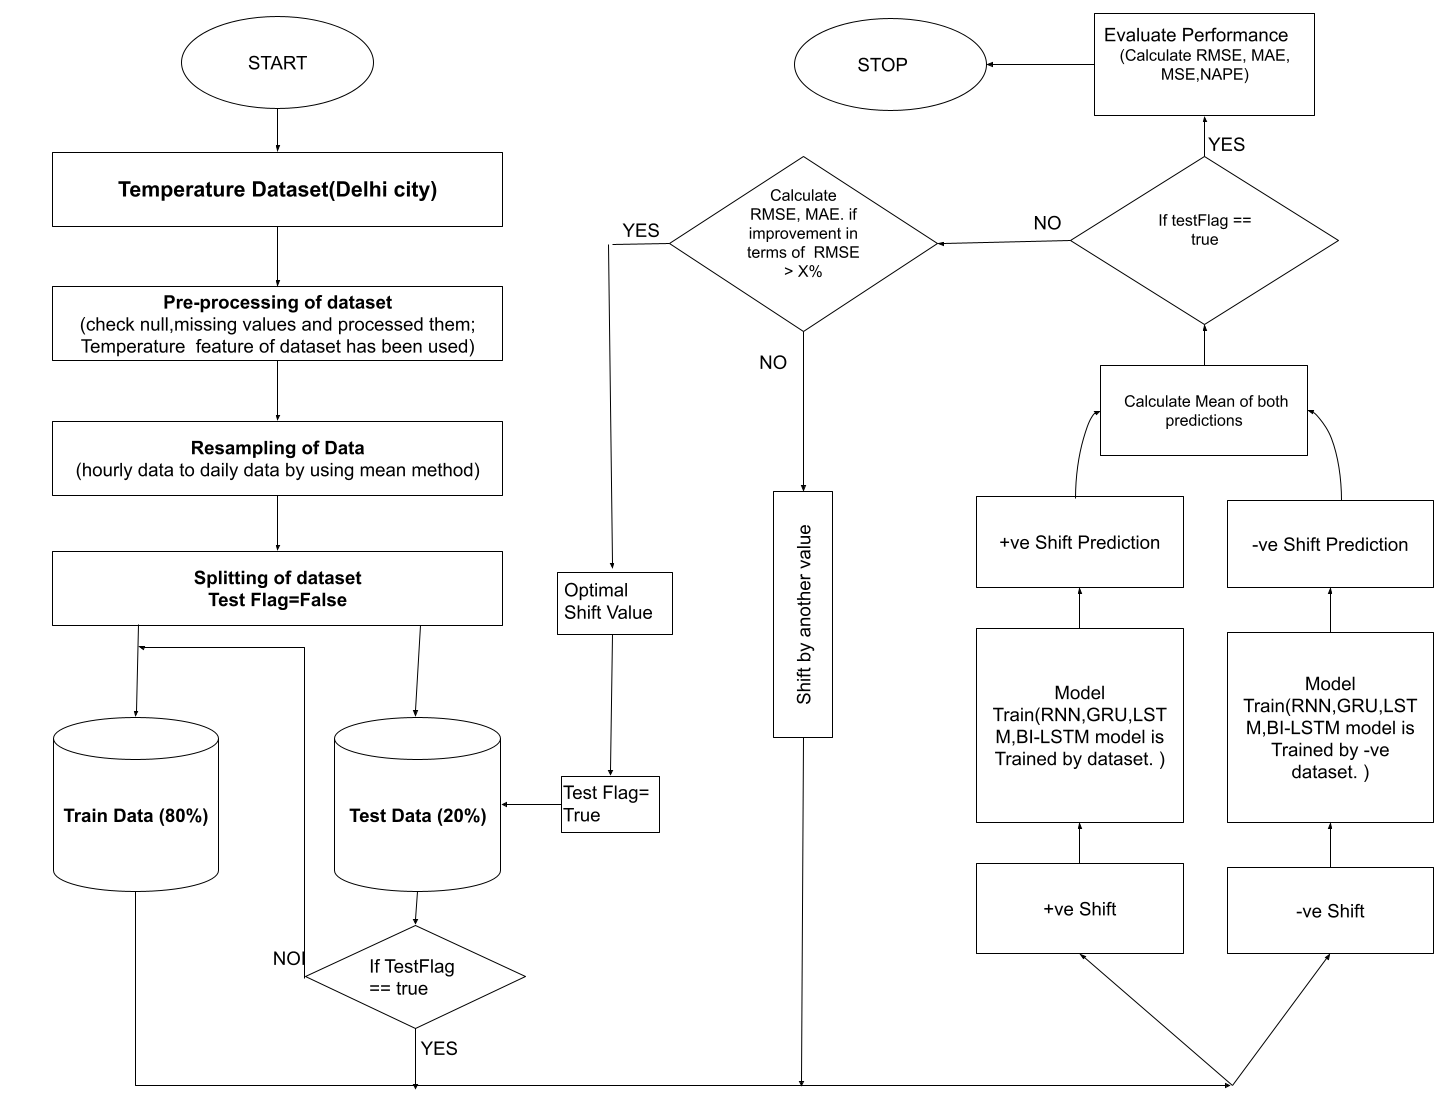
\includegraphics[width=1\textwidth, height=0.9\linewidth]{FlowchartOfjournal.png}
\caption{Framework of the proposed work MBiS-DT + DL models}
\label{fig:Flowchart Of Proposed Work}
\end{figure}
\subsection{Data collection and preprocessing}
\subsubsection{Raw dataset collection}
The Dataset used in this study is publicly accessible on NASA's website (https://power.larc.nasa.gov/data-access-viewer/). The Dataset contains 195101 rows in CSV format of temperature and dew point of New Delhi from 02/01/2001 to 06/04/2023 on an hourly frequency. The T2M are distinct kinds of atmospheric conditions. These conditions define the atmosphere's temperature for each record in the dataset D, shown in eqn. (\ref{eqn:d}).

\begin{equation}
\label{eqn:d}
D=\left \{ x_i, y_i \right \}_{i=1}^{k}
\end{equation}

where, D is denoted as dataset, \(X_i\) is a temperature data of hours interval, and \(Y_i\) its corresponding time. k denotes the number of samples in the dataset, $\forall Y_i  \in Y $ .

\subsubsection{Data preprocessing}
This technique phase consists of four phases. First, dataset D has been resized into a new dimension daily. The function representing the dimension is omega. As shown in eqn. (\ref{eqn:c}), we also organized the data by date and time and examined the Dataset's non-linearity. Furthermore, temperature(T2M) values between 2001 and 2023 have been chosen from the Resized dataset. Each date from January 2, 2001, to April 6, 2023, is placed in the dependent variable column, and each item in that column of time series data for 22 years (2001-2023) having temperature (T2M) as an independent variable column has been added.

\begin{equation}
\label{eqn:c}
D_{new}=\omega \left ( D, p \times q \right )
\end{equation}

where, \(D_{new}\) is the preprocessed the dataset D. Here, p x q are the new dimension of the dataset.
\subsubsection{Exploratory data analysis(EDA)}

% \begin{table*}[h!]
% \caption{statistical summarization of Data set}
% \label{tab: statistical_data_explore }
% \begin{tabular}{ll}
% \hline parameters & Values \\ \hline
% count & 195101 \\
% mean & 25.10 \\
% std & 21.73 \\
% min & -999 \\
% 25\% & 18.70 \\
% 50\% & 26.46 \\
% 75\% & 31.98 \\
% max & 48.79 \\ \hline
% \end{tabular}
% \end{table*}
This section explains statistical details about our Delhi temperature dataset. It provides insights into the Dataset's size, central tendency, variability, distribution, and range. These statistics serve as a foundational resource for analyzing and interpreting temperature trends in Delhi, supporting various climate-related studies, weather forecasts, and informed decision-making processes. The \textbf{"count"} value of 8,128 indicates the Dataset's size, revealing that it bound a substantial number of temperature observations or data points. This size underscores the Dataset's richness and the depth of information available for analysis, offering a robust foundation for temperature-related insights. The \textbf{"mean"} temperature of 25.49 degrees serves as the arithmetic average of the Dataset. It suggests that, on average, the recorded temperatures in Delhi hover around 25.49 degrees. This central tendency measure offers a crucial reference point, representing the typical temperature value within the Dataset. The \textbf{"standard deviation"} (std) of 7.77 quantifies the degree of temperature variation or dispersion in the data. A higher standard deviation indicates more significant variability in the recorded temperatures. In this case, the standard deviation of 7.77 implies that temperature readings in Delhi can exhibit substantial fluctuations around the Mean, signifying the presence of diverse temperature patterns.

The \textbf{"min"} value of 6.95 is the most minor observed temperature in the Dataset. However, this value appears unusual and may require further investigation. Some previous Values, like -999, often signify missing data or anomalies that warrant scrutiny to ensure data quality and integrity, so it is handled by taking the Mean of the successor and predecessor value of the time-series dataset. The \textbf{"max"} value of 41.81 denotes the highest temperature recorded in the Dataset, offering a glimpse into the upper limit of temperature extremes experienced in Delhi. The \textbf{quartile} values—25\% (first quartile), 50\% (median), and 75\% (third quartile)—offer valuable insights into the distribution of temperatures in Delhi. The first quartile at 18.73 indicates that 25\% of temperature readings fall below this level, while the third quartile at 31.48 signifies that 75\% of the temperatures are below this threshold. The median value of 26.85, also the second quartile, represents the middle point of the Dataset when arranged in ascending order. Notably, the median is a robust measure of central tendency unaffected by extreme outliers. These quartile values provide context for understanding the spread and distribution of temperature data in Delhi.



\begin{figure}[ht!]
\centering
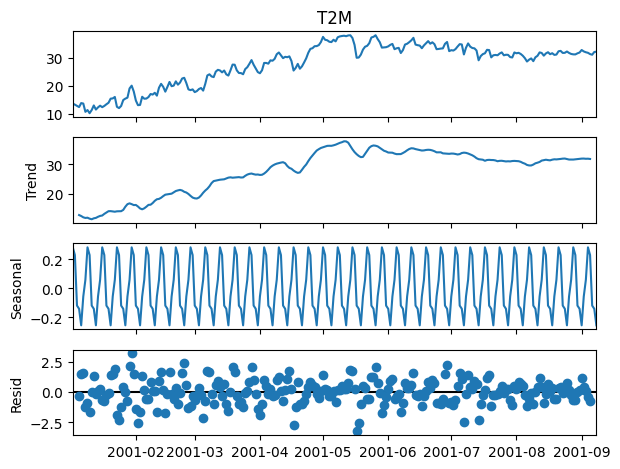
\includegraphics[width=1\textwidth, height=0.75\linewidth]{Graphycal_EDA.png}
\caption{The decomposition of data as a trend, seasonal and residual of Jan. 2001 to Sept. 2001. }
\label{fig:graphycalEDA}
\end{figure}
In our Dataset, a good trend is visualized. A trend represents a substantial and meaningful long-term pattern in temperature variations. This pattern provides the fundamental direction in which the 2-meter air temperature changes over an extended period. In climate science, recognizing such trends is vital for understanding the dynamics of temperature variations over time, whether the moderate warming associated with climate change or the multi-year temperature cycles linked to climate phenomena like Delhi. Accurately identifying and modelling these trends is pivotal for climate scientists and meteorologists, as it enables them to make informed projections about future temperature changes, prepare for potential impacts, and implement mitigation strategies.
In the context of our temperature dataset, "seasonality" represents the regular and cyclical fluctuations in temperature that occur at consistent intervals throughout the year. These fluctuations often align with the changing seasons, resulting in patterns like warmer temperatures during summer and colder temperatures during winter. Seasonality in T2M data can be attributed to various factors, including the tilt of the Earth's axis, which leads to variations in sunlight exposure throughout the year. Identifying seasonality in temperature data is critical for climate scientists and ecologists, as it aids in understanding the impact of changing seasons on ecosystems, agriculture, and human activities. This knowledge is crucial for crop planning, energy demand forecasting, and environmental conservation efforts.

Residuals in our temperature dataset refer to unexplained fluctuations or variations after accounting for the identified trends and seasonality. These residuals represent the difference between the observed 2-meter air temperatures and the values predicted by a model incorporating long-term trends and seasonal patterns. In climate research, analyzing residuals is vital for assessing the accuracy of climate models and identifying any irregular or unanticipated temperature fluctuations. Residuals should exhibit no systematic patterns; if they do, it suggests that the model may need refinement to capture the underlying dynamics of temperature changes better. Effective handling of residuals is essential for producing reliable temperature predictions, which, in turn, inform climate policy, weather forecasts, and resilience planning in the face of temperature-related challenges.
% \subsection{Train, and Test Splitting of Dataset}



% \par {\textbf{Step 4}: Applying Deep Learning Models:}\\ the model \(\emptyset\left(D_{Tr}\ ,\ D_{Te}\right)\) has been applied. The forecasting for the test sample has been obtained in the model's training and test part. Prediction is obtained:\(\left\{P_i^\emptyset\right\}_i^m\), where m is number of test sample %\cite{hrithik2022classification}.

% \par {\textbf{Step 5}: Root Mean Squared Error:}\\ RMSE is calculated by eqn. \ref{eqn:e}.



% Where N is total no of test Sample, \(\hat{y_{i}}\) is a predicted data of model, and \(y_{i}\) is the actual test deta.\\
% \par {\textbf{Step 6}: Proposed Technique:} \\
\subsection{Proposed Multi-Bidirectional shifting based Data transformation(MBiS-DT) with DL model}
\begin{figure}[ht!]
\centering
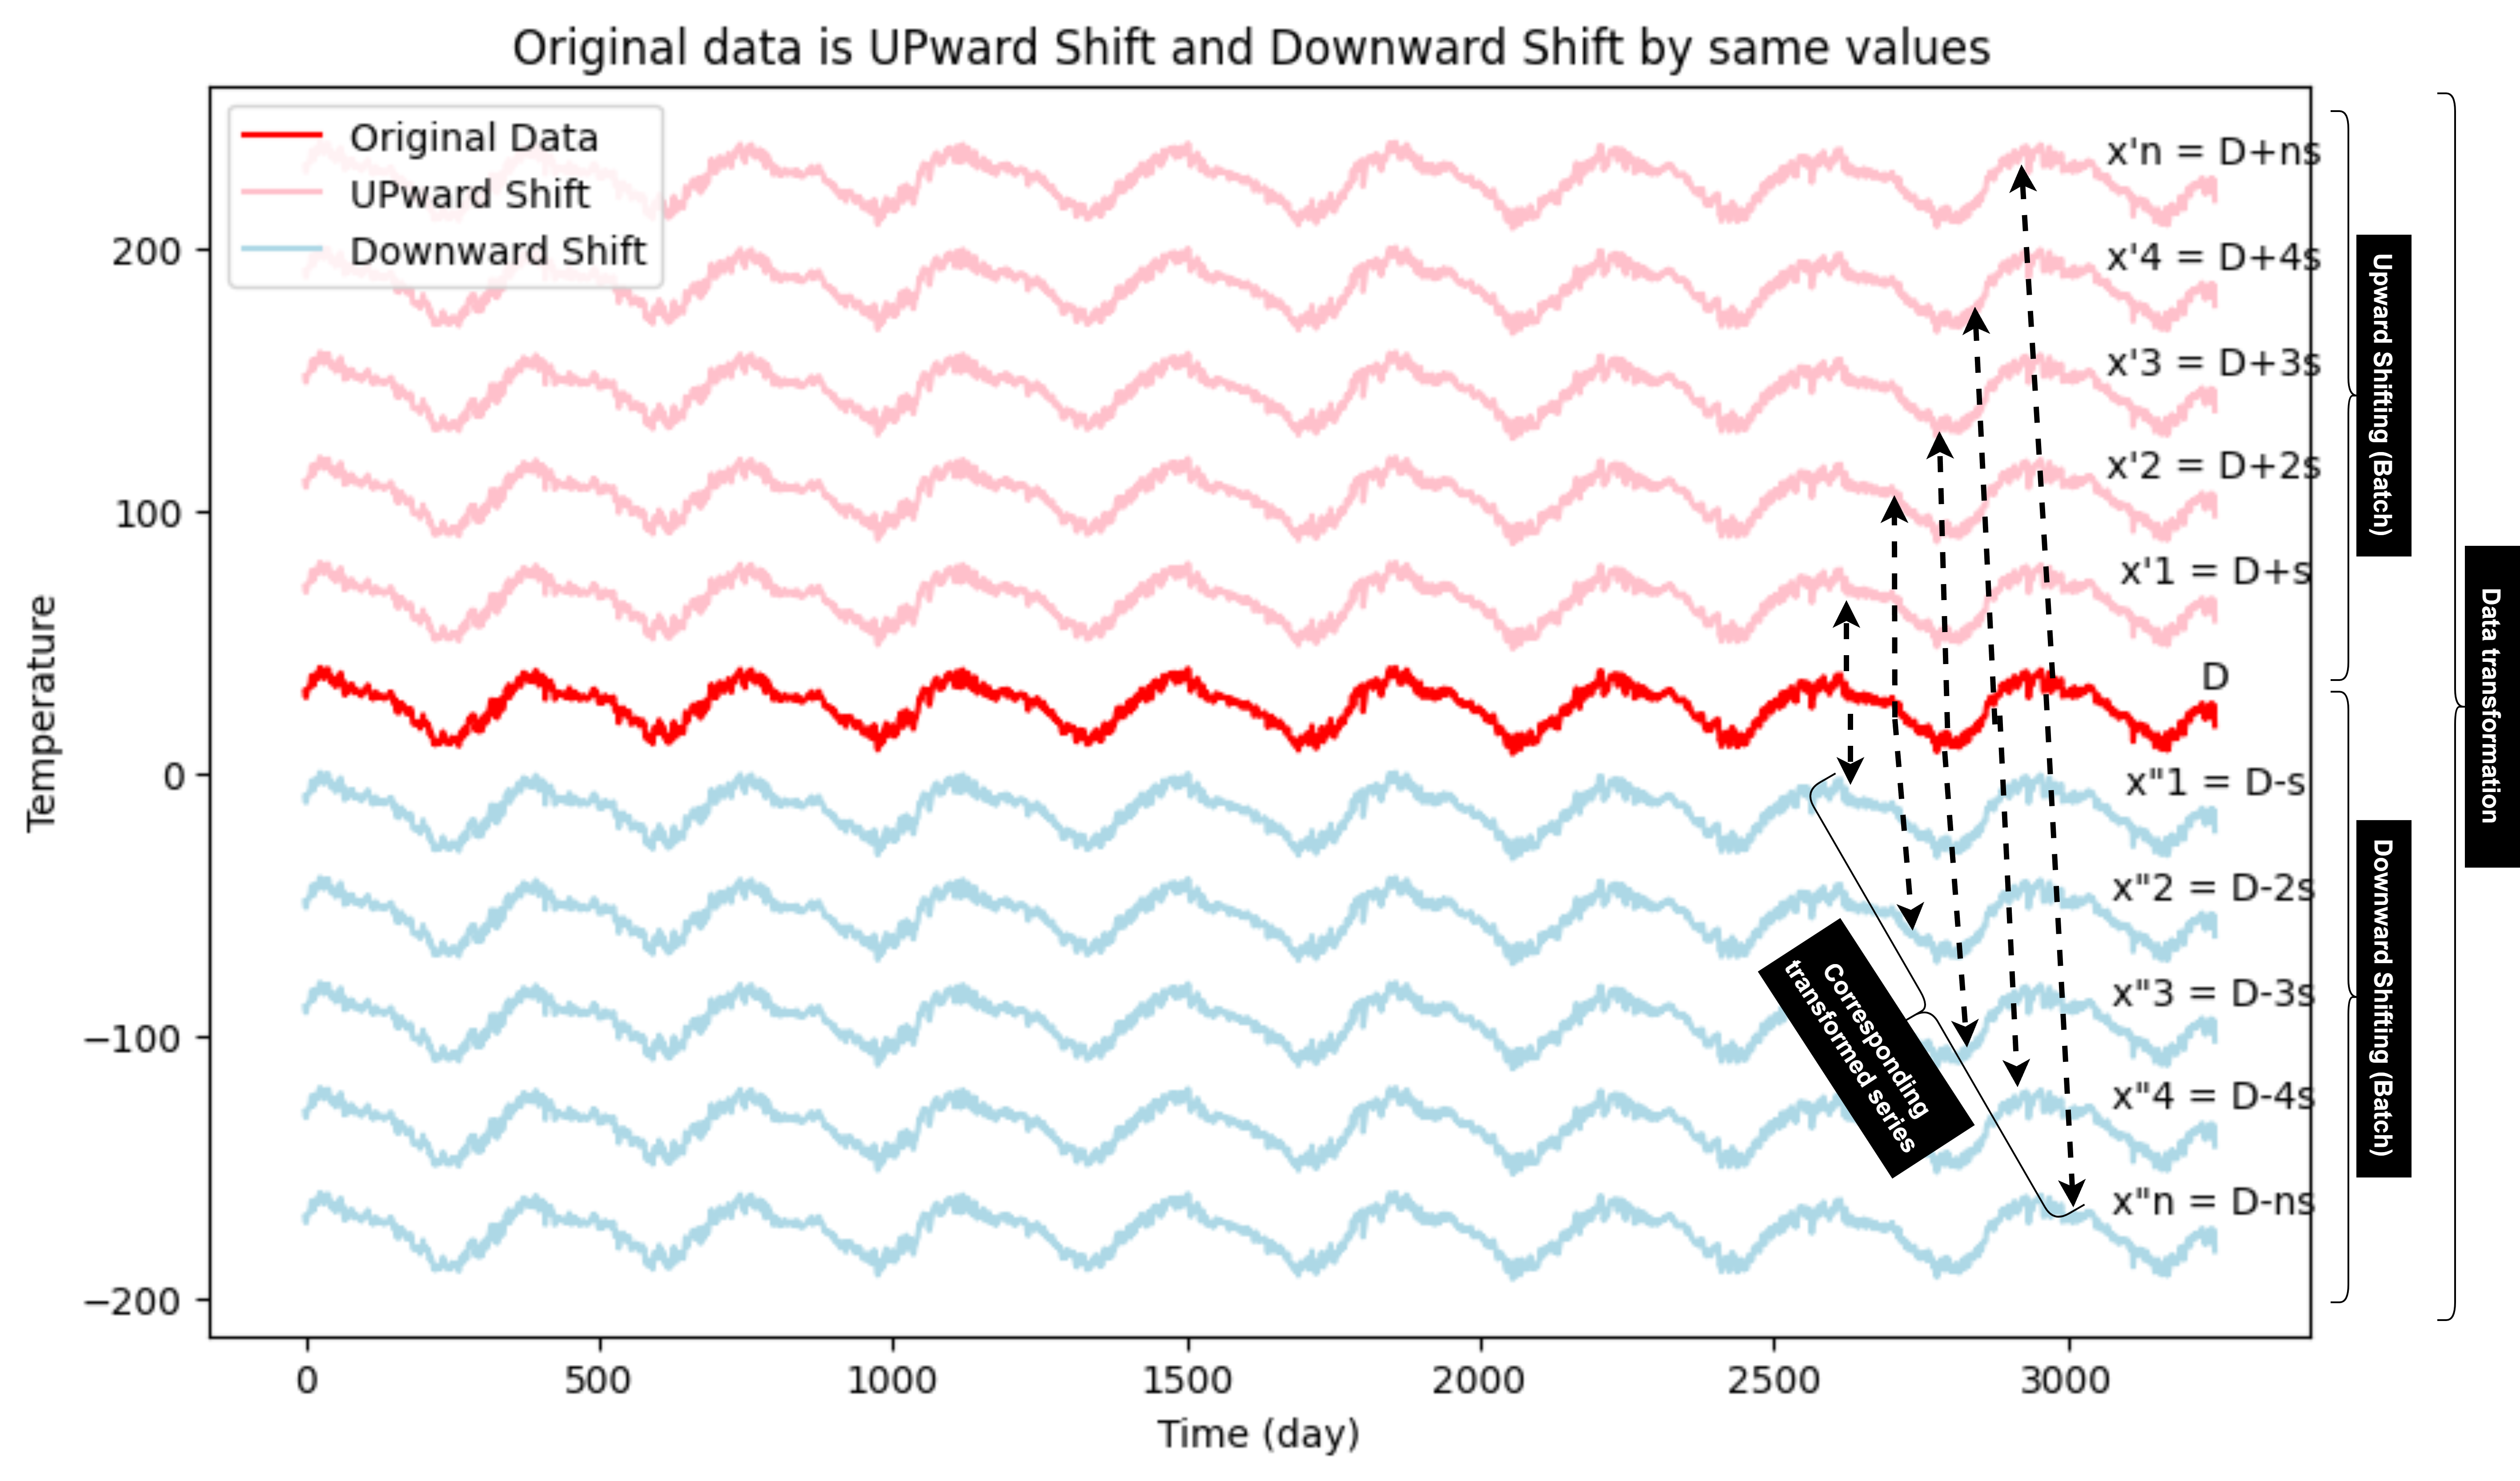
\includegraphics[scale = 0.4]{shifted_dataset.png}
\caption{Pictorial representation of Multi-Bidirectional shifting based Data Transformation(MBiS-DT) for multiple DL learning for ensemble of models.}
\label{fig:shifted_dataset}
\end{figure}
The preprocessed dataset has been divided into two parts: training \((T_{train})\) (80\%) and testing \((T_{test})\) (20\%). The dataset is mutually exclusive in eqn. (\ref{eqn:a}) and exhaustive in eqn. (\ref{eqn:b}).

\begin{equation}
\label{eqn:a}
D_{Tr}\cup D_{Te}=D_{T}
\end{equation}

\begin{equation}
\label{eqn:b}
\left \{ D_{Tr} \cap D_{Te} \right \}=\varnothing
\end{equation}

For the data points $x_i$ in the training dataset $D_{Tr}$, two series can be created as in eqn. (\ref{eqn:01}):
\begin{equation}
\begin{aligned}
\label{eqn:01}
\{x_i^{\prime}=x_i+s\}_{i=1}^n \\
\{x_i^{\prime\prime}=x_i-s\}_{i=1}^n \; \forall x_i \in D_{Tr}
\end{aligned}
\end{equation}
where $s \in Z$ and $x_i^{\prime}$ and $x_{i}^{\prime\prime}$ depicts the positive and negative series obtained by shifting the series with positive and negative values of the step length $s$ of the shift. The series has been prepared for $n$ number of iterations.
Predictions for both the positive $x_i^{\prime}$ and negative $x_i^{\prime\prime}$ series has been obtained as $\hat{y}_i^{\prime}$ and $ \hat{y}_i^{\prime\prime}$ respectively.
The predictions are combined to form a final set of predictions using eqn. (\ref{eqn:02}), which is utilized for the comparison with the actual values of training dataset $D_{Tr}$ .
\begin{equation}
\label{eqn:02}
\hat{y}_{final}=\frac{y_i^{\prime}+y_i^{\prime\prime}}{2}
\end{equation}
where $\hat{y}_{final}$ represents the final prediction. The above procedure is repeated for $n$-number of iterations, and an optimal value of $s$ is obtained for which the RMSE is best out of $n$-number of iterations.
Then, the model is trained for the actual training data $D_{Tr}$, and predictions are obtained for the test data $D_{Te}$, which is $D_{Te}^{\prime}$. Further, two positive and negative series are obtained from test prediction $D_{Te}^{\prime}$ as reflected in eqn. (\ref{eqn:03}).
\begin{equation}
\begin{aligned}
\label{eqn:03}
\{x_j^{\prime}=x_j+s\} \\
\{x_j^{\prime\prime}=x_j-s\} \; \forall x_j \in D_{Te}^{\prime}
\end{aligned}
\end{equation}
where $s$ is the step length obtained earlier and $x_j^{\prime}$ and $x_{j}^{\prime\prime}$ depicts the positive and negative series obtained by shifting the series with positive and negative values of the step length $s$ of the test predictions $ D_{Te}^{\prime}$.
Predictions for both the positive $x_j^{\prime}$ and negative $x_j^{\prime\prime}$ series has been obtained as $ \hat{y}_j^{\prime}$ and $ \hat{y}_j^{\prime\prime}$ respectively.

The predictions are combined to form a final set of predictions using eqn. (\ref{eqn:04}), which is utilized for the comparison with the actual values of training dataset $D_{Te}$
\begin{equation}
\label{eqn:04}
\hat{y}_{final}^{\prime}=\frac{\hat{y}_j^{\prime}+\hat{y}_j^{\prime\prime}}{2}
\end{equation}
where $\hat{y}_{final}^{\prime}$ represents the final prediction.




% \begin{figure}[ht!]
% %\centering
% \subfloat[Test data vs Proposed MBiS-DT GRU] {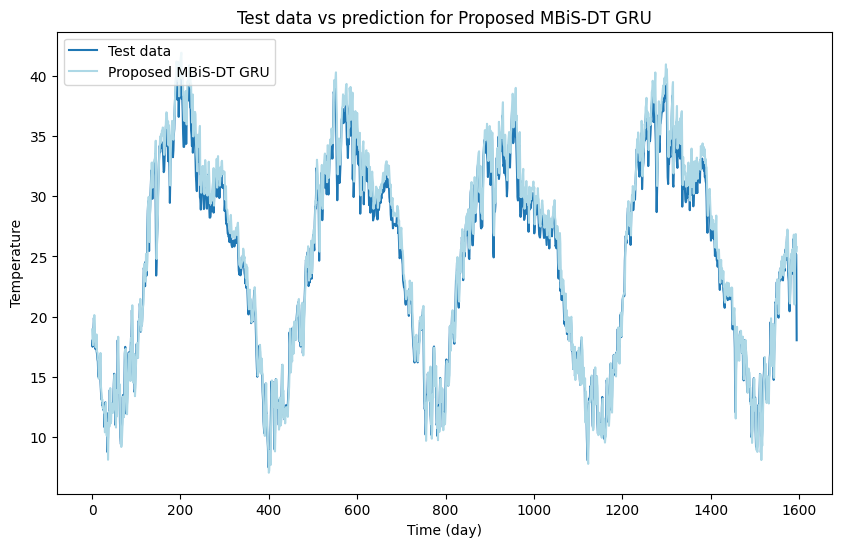
\includegraphics[scale=0.3]{testData_vs_proposed_GRU.png}\label{fig:BarPlot_TestDataVSMBiS-DT_GRU}}
% \hfill
% \subfloat[Test data vs Proposed MBiS-DT RNN]{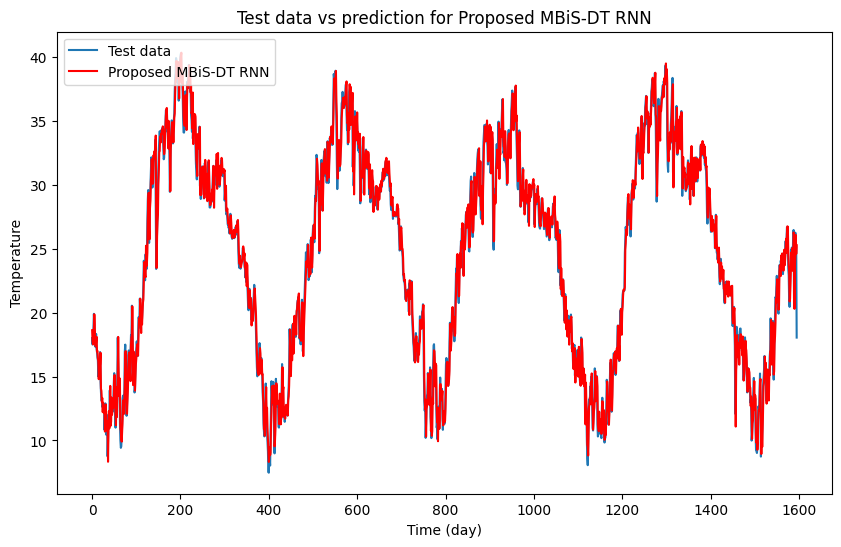
\includegraphics[scale=0.3]{testData_vs_proposed_RNN.png}\label{fig:BarPlot_TestDataVSMBiS-DT_RNN}}\\
% \subfloat[Test data vs Proposed MBiS-DT BI-LSTM]{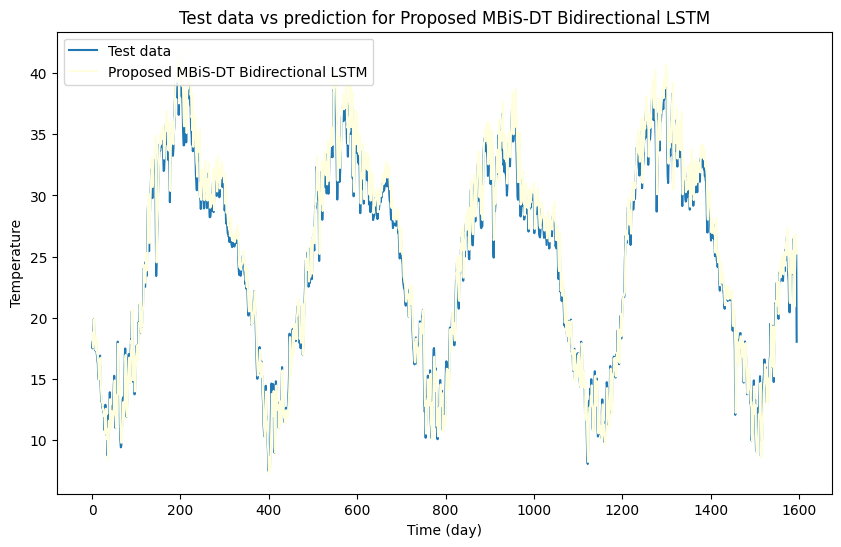
\includegraphics[scale=0.3]{testData_vs_proposed_BI-lstm.png}\label{fig:BarPlot_TestDataVSMBiS-DT_BILSTM}}
% \hfill
% \subfloat[Test data vs Proposed MBiS-DT LSTM]{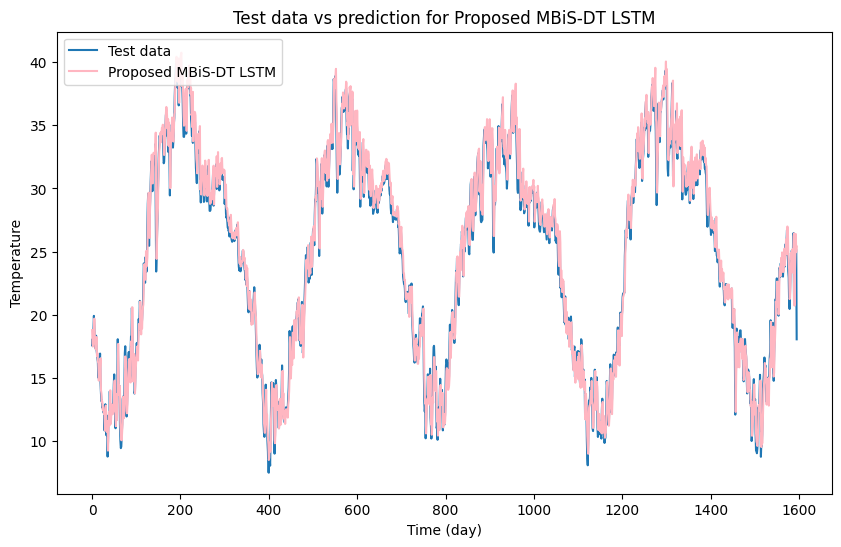
\includegraphics[scale=0.3]{testData_vs_proposed_LSTM.png}\label{fig:BarPlot_TestDataVSMBiS-DT_LSTM}}
% \caption{Prediction plot of original test data(subset) and corresponding to traditional DL models and proposed MBiS-DT + DL's models.}
% \label{fig:Line plot of vs proposed MBiS-DT models}
% \end{figure}
    


% \begin{figure}[ht!]
% \centering
% 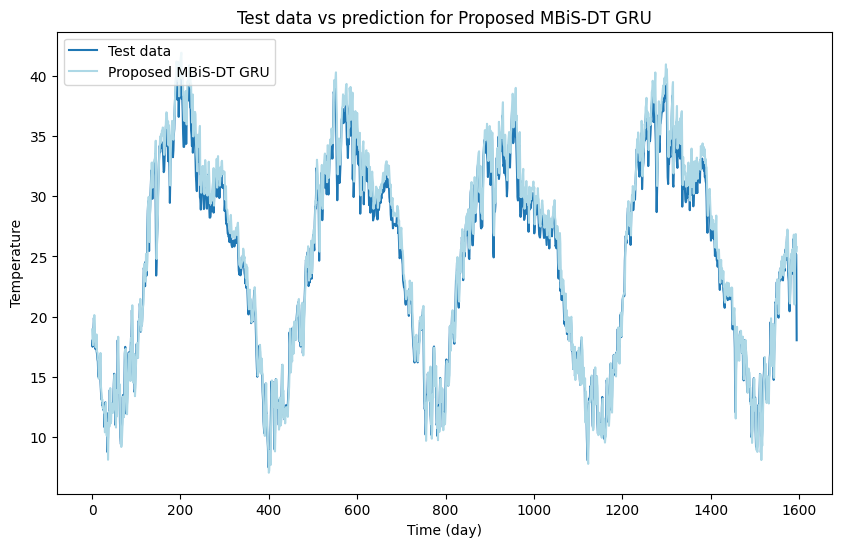
\includegraphics[width=1\textwidth, height=0.9\linewidth]{testData_vs_proposed_GRU.png}
% \caption{Test data vs Proposed MBiS-DT GRU}
% \label{fig:BarPlot_TestDataVSMBiS-DT_GRU}
% \end{figure}
% \begin{figure}[ht!]
% \centering
% 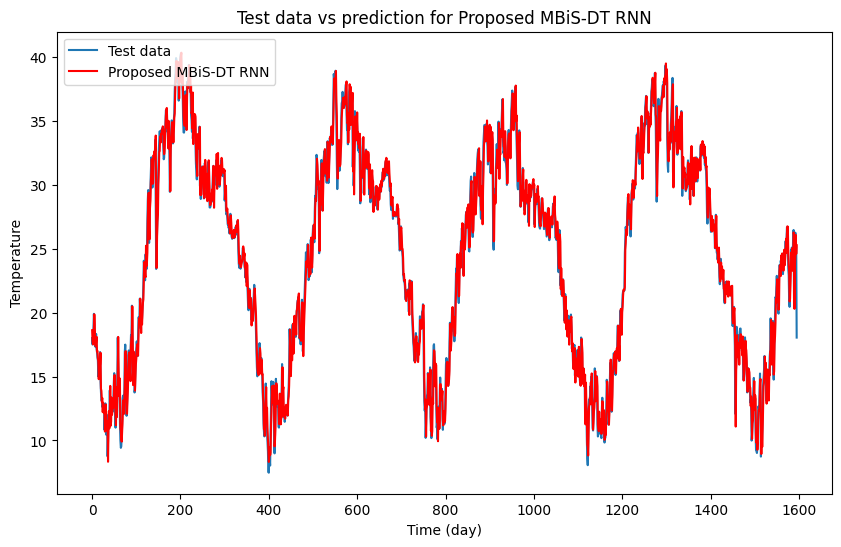
\includegraphics[width=1\textwidth, height=0.9\linewidth]{testData_vs_proposed_RNN.png}
% \caption{Test data vs Proposed MBiS-DT RNN}
% \label{fig:BarPlot_TestDataVSMBiS-DT_RNN}
% \end{figure}
% \begin{figure}[ht!]
% \centering
% 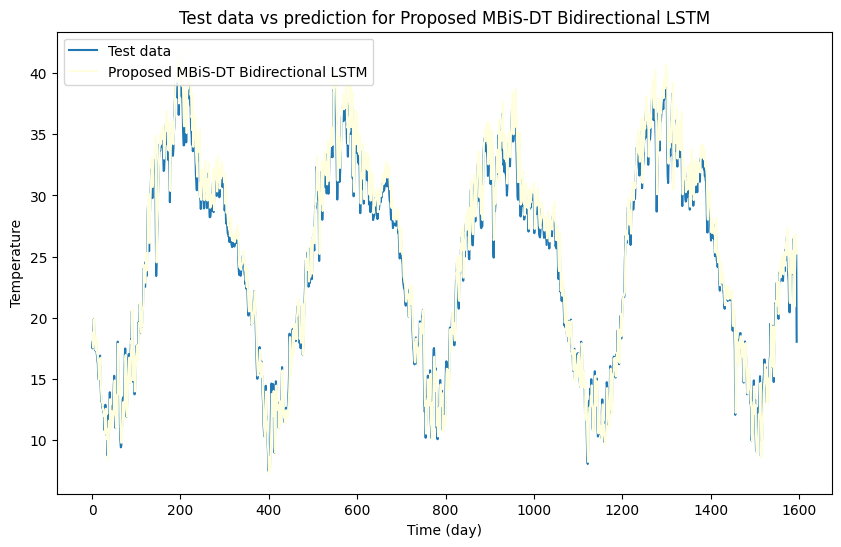
\includegraphics[width=1\textwidth, height=0.9\linewidth]{testData_vs_proposed_BI-lstm.png}
% \caption{Test data vs Proposed MBiS-DT BI-LSTM}
% \label{fig:BarPlot_TestDataVSMBiS-DT_BILSTM}
% \end{figure}
% \begin{figure}[ht!]
% \centering
% 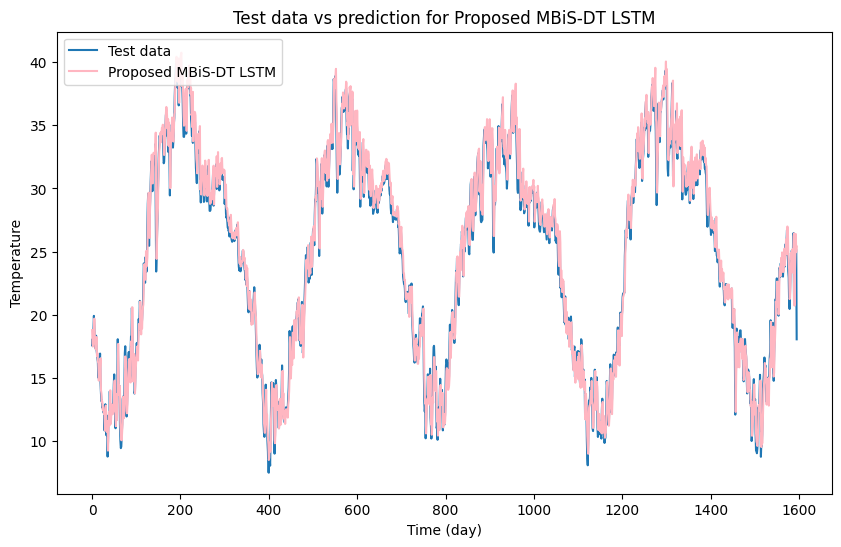
\includegraphics[width=1\textwidth, height=0.9\linewidth]{testData_vs_proposed_LSTM.png}
% \caption{Test data vs Proposed MBiS-DT LSTM}
% \label{fig:BarPlot_TestDataVSMBiS-DT_LSTM}
% \end{figure}



% \begin{figure}[ht!]
% %\centering
% \subfloat[Test data vs Proposed MBiS-DT GRU] {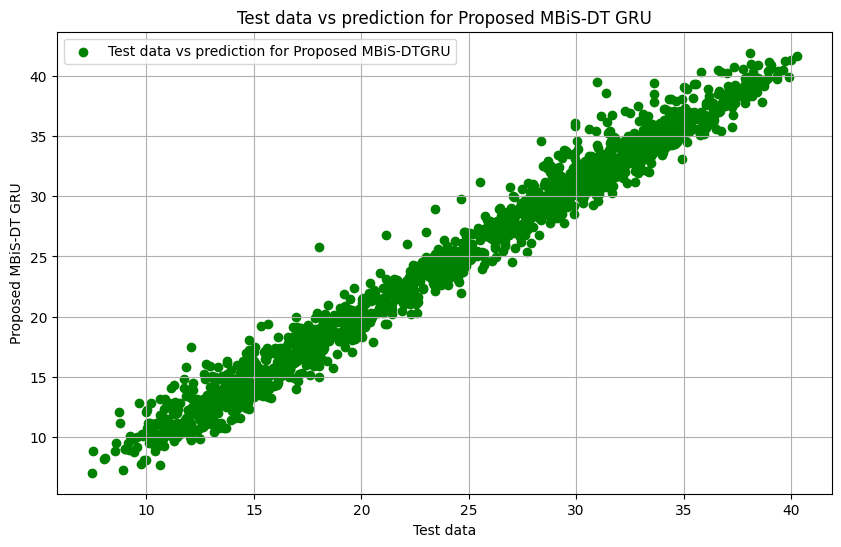
\includegraphics[scale=0.3]{scatter_gru.png}\label{fig:ScatterPlot_TestDataVSMBiS-DT_GRU}}
% \hfill
% \subfloat[Test data vs Proposed MBiS-DT RNN]{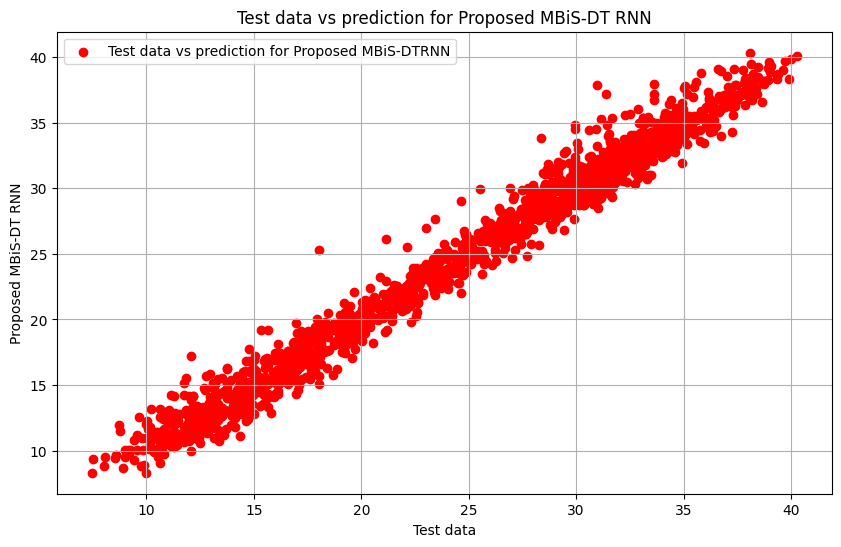
\includegraphics[scale=0.3]{scatter_rnn.png}\label{fig:ScatterPlot_TestDataVSMBiS-DT_RNN}}\\
% \subfloat[Test data vs Proposed MBiS-DT BI-LSTM]{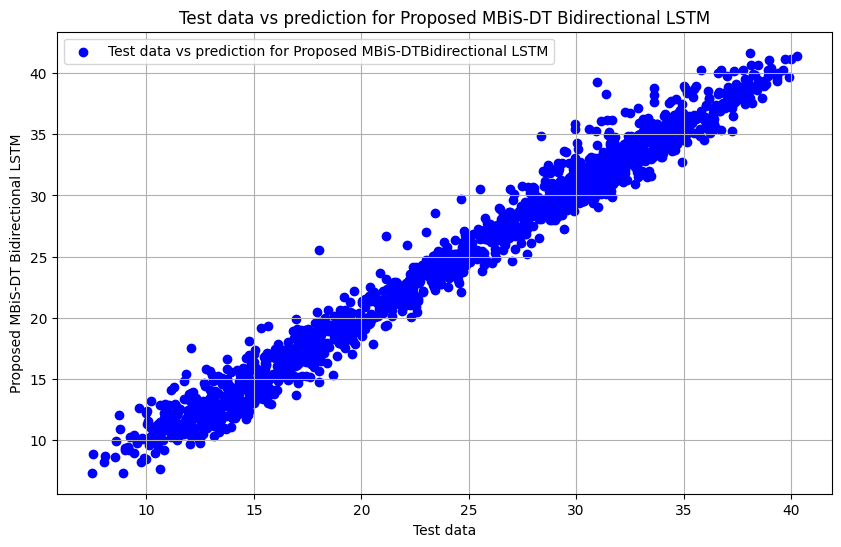
\includegraphics[scale=0.3]{scatter_bilstm.png}\label{fig:ScatterPlot_TestDataVSMBiS-DT_BI-LSTM}}
% \hfill
% \subfloat[Test data vs Proposed MBiS-DT LSTM]{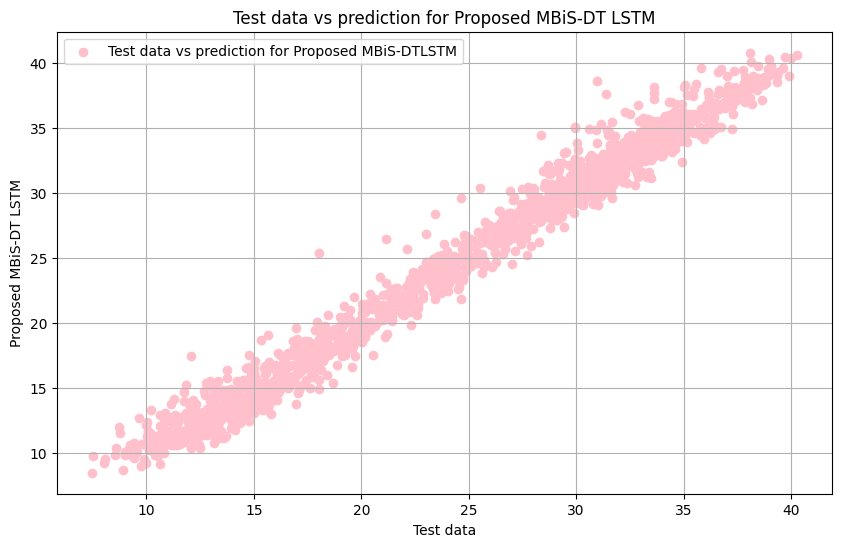
\includegraphics[scale=0.3]{scatter_lstm.png}\label{fig:ScatterPlot_TestDataVSMBiS-DT_LSTM}}
% \caption{Superimposed Prediction Scattered plot of traditional DL and proposed model over test data.}
% \label{fig:Scatter plot of vs proposed MBiS-DT models}
% \end{figure}




% \begin{figure}[ht!]
% \centering
% 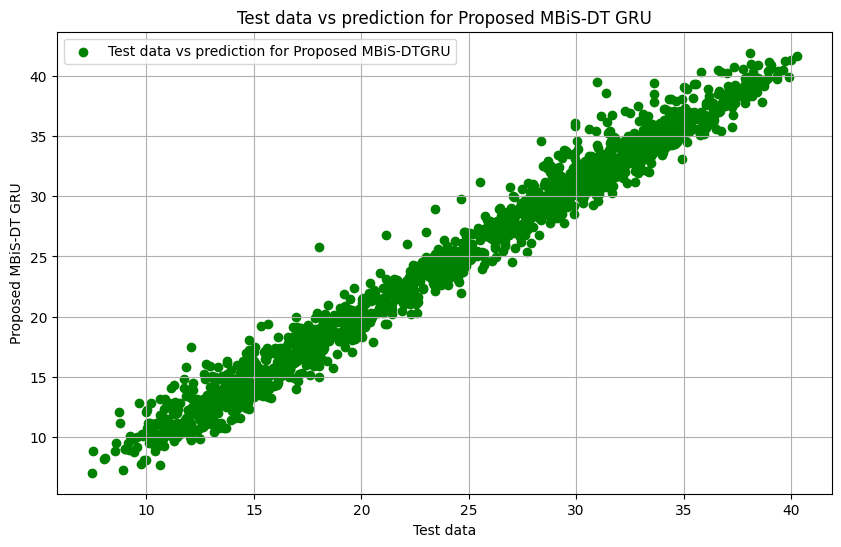
\includegraphics[width=1\textwidth, height=0.9\linewidth]{scatter_gru.png}
% \caption{Test data vs Proposed MBiS-DT GRU}
% \label{fig:ScatterPlot_TestDataVSMBiS-DT_GRU}
% \end{figure}
% \begin{figure}[ht!]
% \centering
% 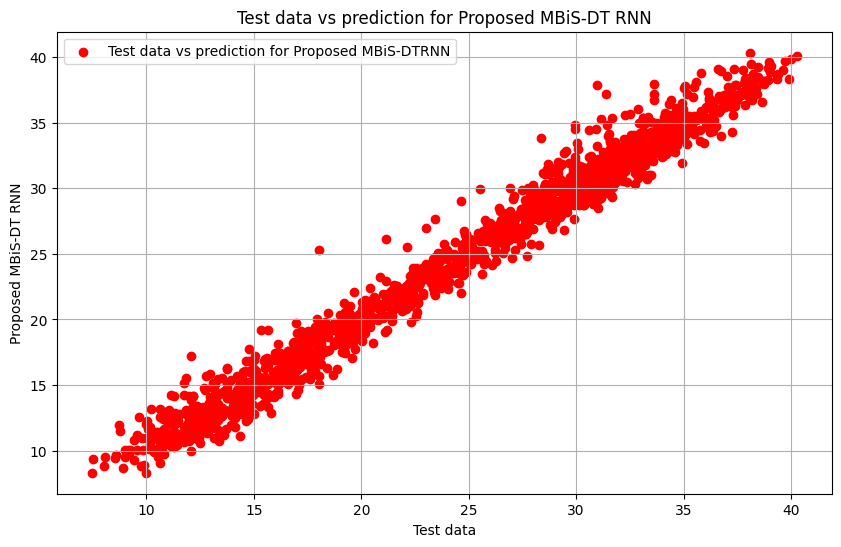
\includegraphics[width=1\textwidth, height=0.9\linewidth]{scatter_rnn.png}
% \caption{Test data vs Proposed MBiS-DT RNN}
% \label{fig:ScatterPlot_TestDataVSMBiS-DT_RNN}
% \end{figure}
% \begin{figure}[ht!]
% \centering
% 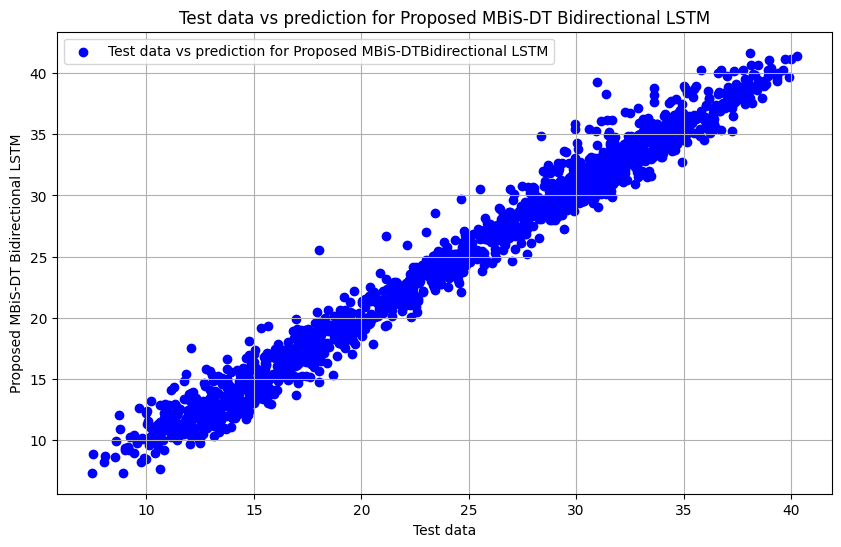
\includegraphics[width=1\textwidth, height=0.9\linewidth]{scatter_bilstm.png}
% \caption{Test data vs Proposed MBiS-DT BI-LSTM}
% \label{fig:ScatterPlot_TestDataVSMBiS-DT_BI-LSTM}
% \end{figure}
% \begin{figure}[ht!]
% \centering
% 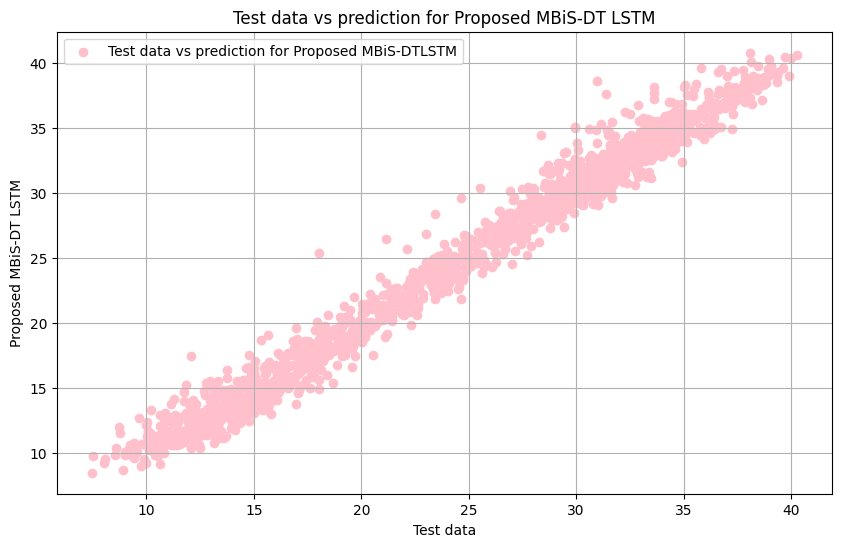
\includegraphics[width=1\textwidth, height=0.9\linewidth]{scatter_lstm.png}
% \caption{Test data vs Proposed MBiS-DT LSTM}
% \label{fig:ScatterPlot_TestDataVSMBiS-DT_LSTM}
% \end{figure}




\subsection{Performance Measures:}
\subsubsection{Root Mean Squared Error (RMSE):}
This performance metric is used widely in regression tasks, including temperature prediction. It calculates the average magnitude of the errors between actual and predicted values. The RMSE is calculated by taking the square root of the average of the squared differences between actual and predicted values.

The formula for RMSE is as in eqn. (\ref{eqn:e}):
\begin{equation}
\label{eqn:e}
RMSE = \sqrt {\frac{1}{N} \sum_{i=1}^{N} (\hat{y_{i}} - y_{i})^2}
\end{equation}
where the variables $\hat{y}_i$ is predicted values of the target variable (e.g., temperature), $y_i$ is the actual values of the target variable, and N is the total number of data point in the Dataset.
\subsubsection{Mean Absolute Error (MAE):} It is a data-dependent performance metric used to evaluate the average exact error between actual and predicted variables. The formula for MAE is depicted in eqn. (\ref{eqn:mae})
\begin{equation}
\label{eqn:mae}
MAE = \frac{1}{N} \sum_{i=1}^{N} \left|\hat{y_{i}} - y_{i}\right| .
\end{equation}
where the variables $\hat{y}_i$ are predicted values of the target variable (e.g., temperature), $y_i$ are the actual values of the target variable, and N is the total no. of the data point in Dataset.

\subsubsection{Mean Squared Error (MSE):}
Mean Squared Error (MSE) is another widely used performance metric in regression tasks, including temperature prediction. It computes the Mean of the squared differences between actual and predicted values. MSE emphasizes a more significant error value than a more minor error value due to the squaring of the differences.
The formula for MSE is as depicted in eqn. (\ref{eqn:mse})
\begin{equation}
\label{eqn:mse}
MSE = \frac{1}{N} \sum_{i=1}^{N} (\hat{y_{i}} - y_{i})^2
\end{equation}
where the variables $\hat{y}_i$ are predicted values of the target variable (e.g., temperature), $y_i$ are the actual values of the target variable, and N is the number of data points in the Dataset.


\subsubsection{Mean Absolute Percentage Error (MAPE):}
Mean Absolute Percentage Error (MAPE) is a performance metric commonly used in regression tasks, including temperature prediction. It measures the average percentage difference between predicted and actual values, providing a relative measure of the accuracy of the model's predictions.

The formula for MAPE is represented in eqn. (\ref{eqn:mape})
\begin{equation}
\label{eqn:mape}
MAPE = \frac{100}{N} \sum_{i=1}^{N} \left|(\frac{\hat{y_{i}} - y_{i}}{y_i})\right| .
\end{equation}

%MAPE = (1/n) * Σ(|(y_actual - y_pred) / y_actual|) * 100

where the variables $\hat{y}_i$ are predicted values of the target variable (e.g., temperature), $y_i$ are the actual values of the target variable, and N is the number of data points in the Dataset.



\subsection{Implamentation setup and parameters settings}
The various packages of Python are utilized to implement the baseline and proposed models. These include Pandas (v1.5.3), Scikit-Learn (v1.2.2) for model creation and performance analysis, Keras (v2.12.0), TensorFlow (v2.12.0) for Keras backend, and NumPy (v1.23.5) for exploratory data analysis, and For describing the findings and creating graphs, we used Plotly (v5.14.1), seaborn (v0.12.2), and Matplotlib (v3.7.1). To create flowcharts, it has also used \href{https: //app.diagrams.net/}{https: //app.diagrams.net/}. One system was employed for the experiments: a MacOS-based computer with Apple M1 having 8 GB RAM. All experiments were done on Google Colab with runtime Python 3 and hardware-accelerated T4 GPU with 12.7 GB RAM. Table \ref{tab: my-table} has the parameter values of traditional DL model and proposed model.

\begin{table*}[h!]
\centering
\caption{Parameter setting of traditional DL models and proposed MBiS-DT Models}
\label{tab: my-table}
\begin{tabular}{ll}
\hline Hyperparameters & Values \\ \hline
Batch Size & 32 \\
Optimizer & Adam \\
Loss function & Mean Squared Error \\
Epoch & 200 with early stopping \\
training size & 0.8 \\ \hline
\end{tabular}
\end{table*}
Upward batch and Downward batch ensemble(UD-Batch) and Corresponding upward and downward ensemble(CUD-ensemble)
\section{Results and Discussion}\label{sec2}
In this paper Upward batch and Downward batch ensemble(UD-Batch) is used. in UD-Batch ensemble first we shifted the dataset n times upward and n times downward with same step value then we apply traditional DL models  on upper shifted datasets and ensemble the predictions similerly done for downward shifted datasets  to get the downward prediction and at the last we ensemble the upword  prediction and downword prediction. There is  also a second approach called Corresponding upward and downward ensemble(CUD-ensemble) in which we ensemble the individual upshifted prediction and downshifted prediction  and then take average of all individual prediction. In fig. \ref{fig:all_models_mae}, fig.\ref{fig:all_models_rmse}, fig.\ref{fig:all_models_mse}, fig.\ref{fig:all_models_mape} dark area showing the MAE, RMSE, MSE, MAPE of UD-Batch ensemble  respectively and light area showing the MAE, RMSE, MSE, MAPE of UD-Batch ensemble  respectively so here clearly shown that UD-Batch ensemble more precise then CUD-ensemble.
\begin{figure}[ht!]
%\centering
\subfloat[LSTM: UD-Batch ensemble Vs CUD ensemble] {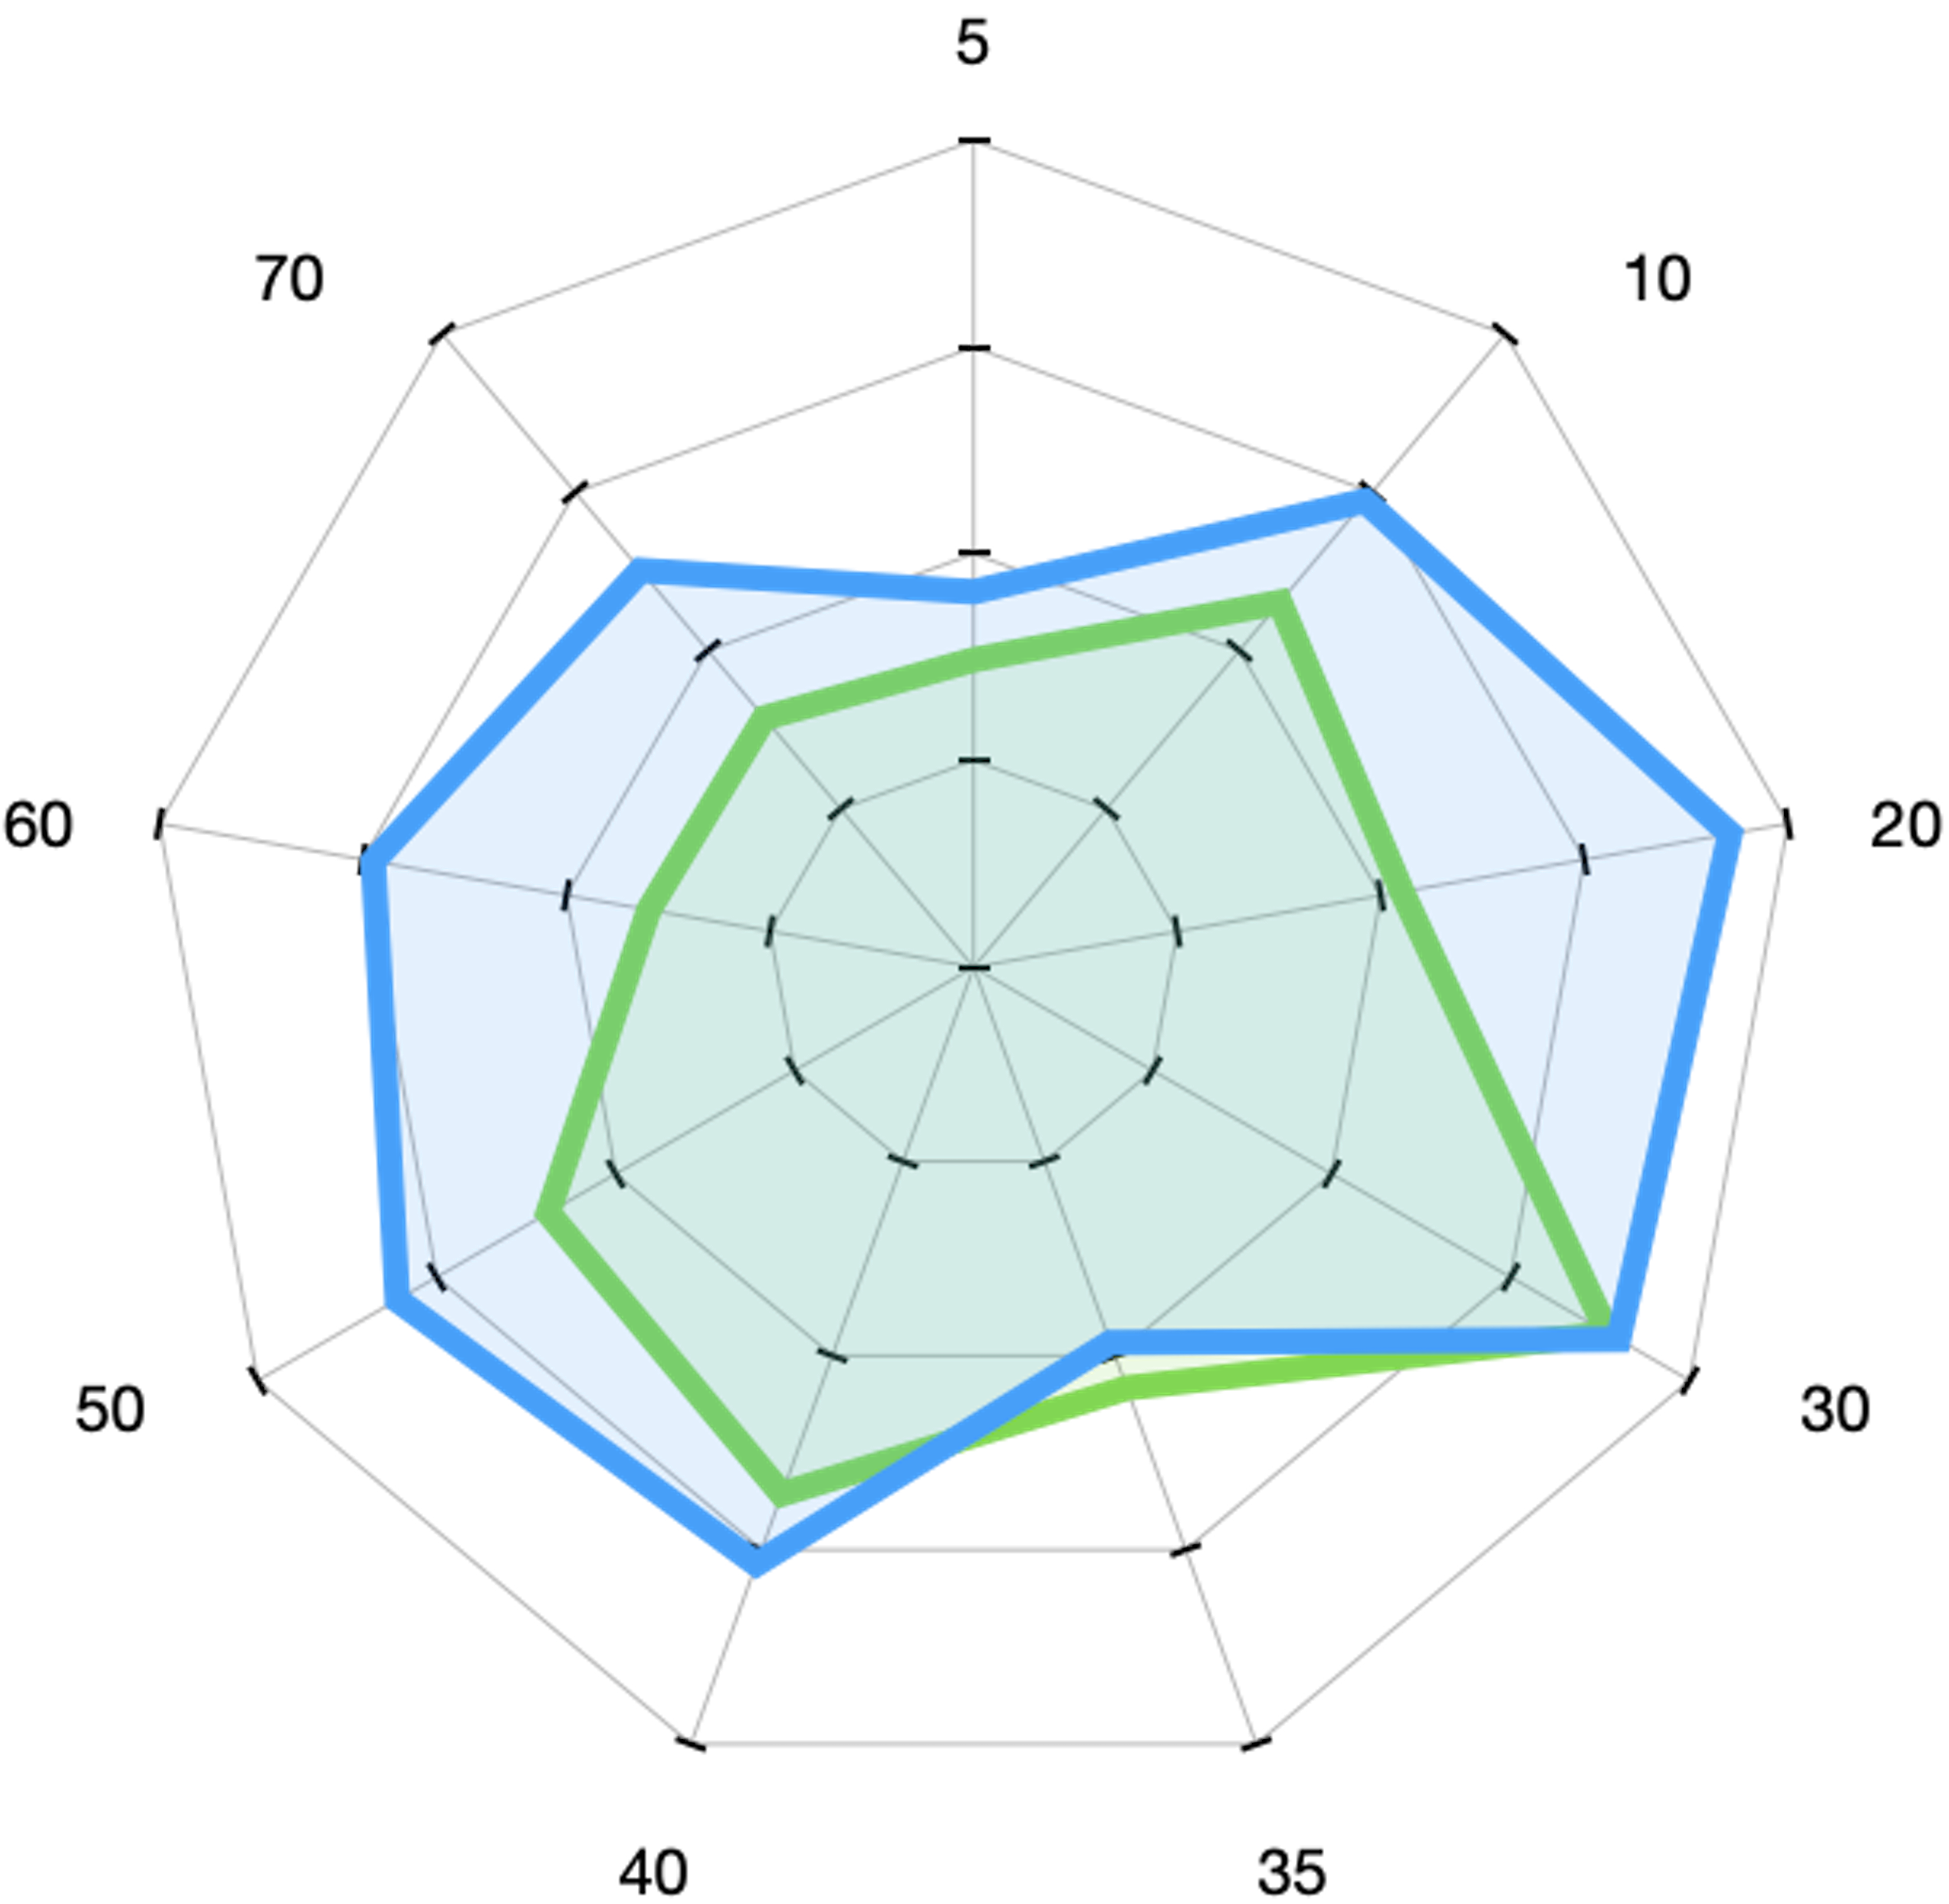
\includegraphics[width=0.4\textwidth, height=0.25\linewidth]{LSTM_MAE_SPIDER.png}\label{fig:LSTM MAE SPIDER}}
\hfill
\subfloat[RNN: UD-Batch ensemble Vs CUD ensemble]{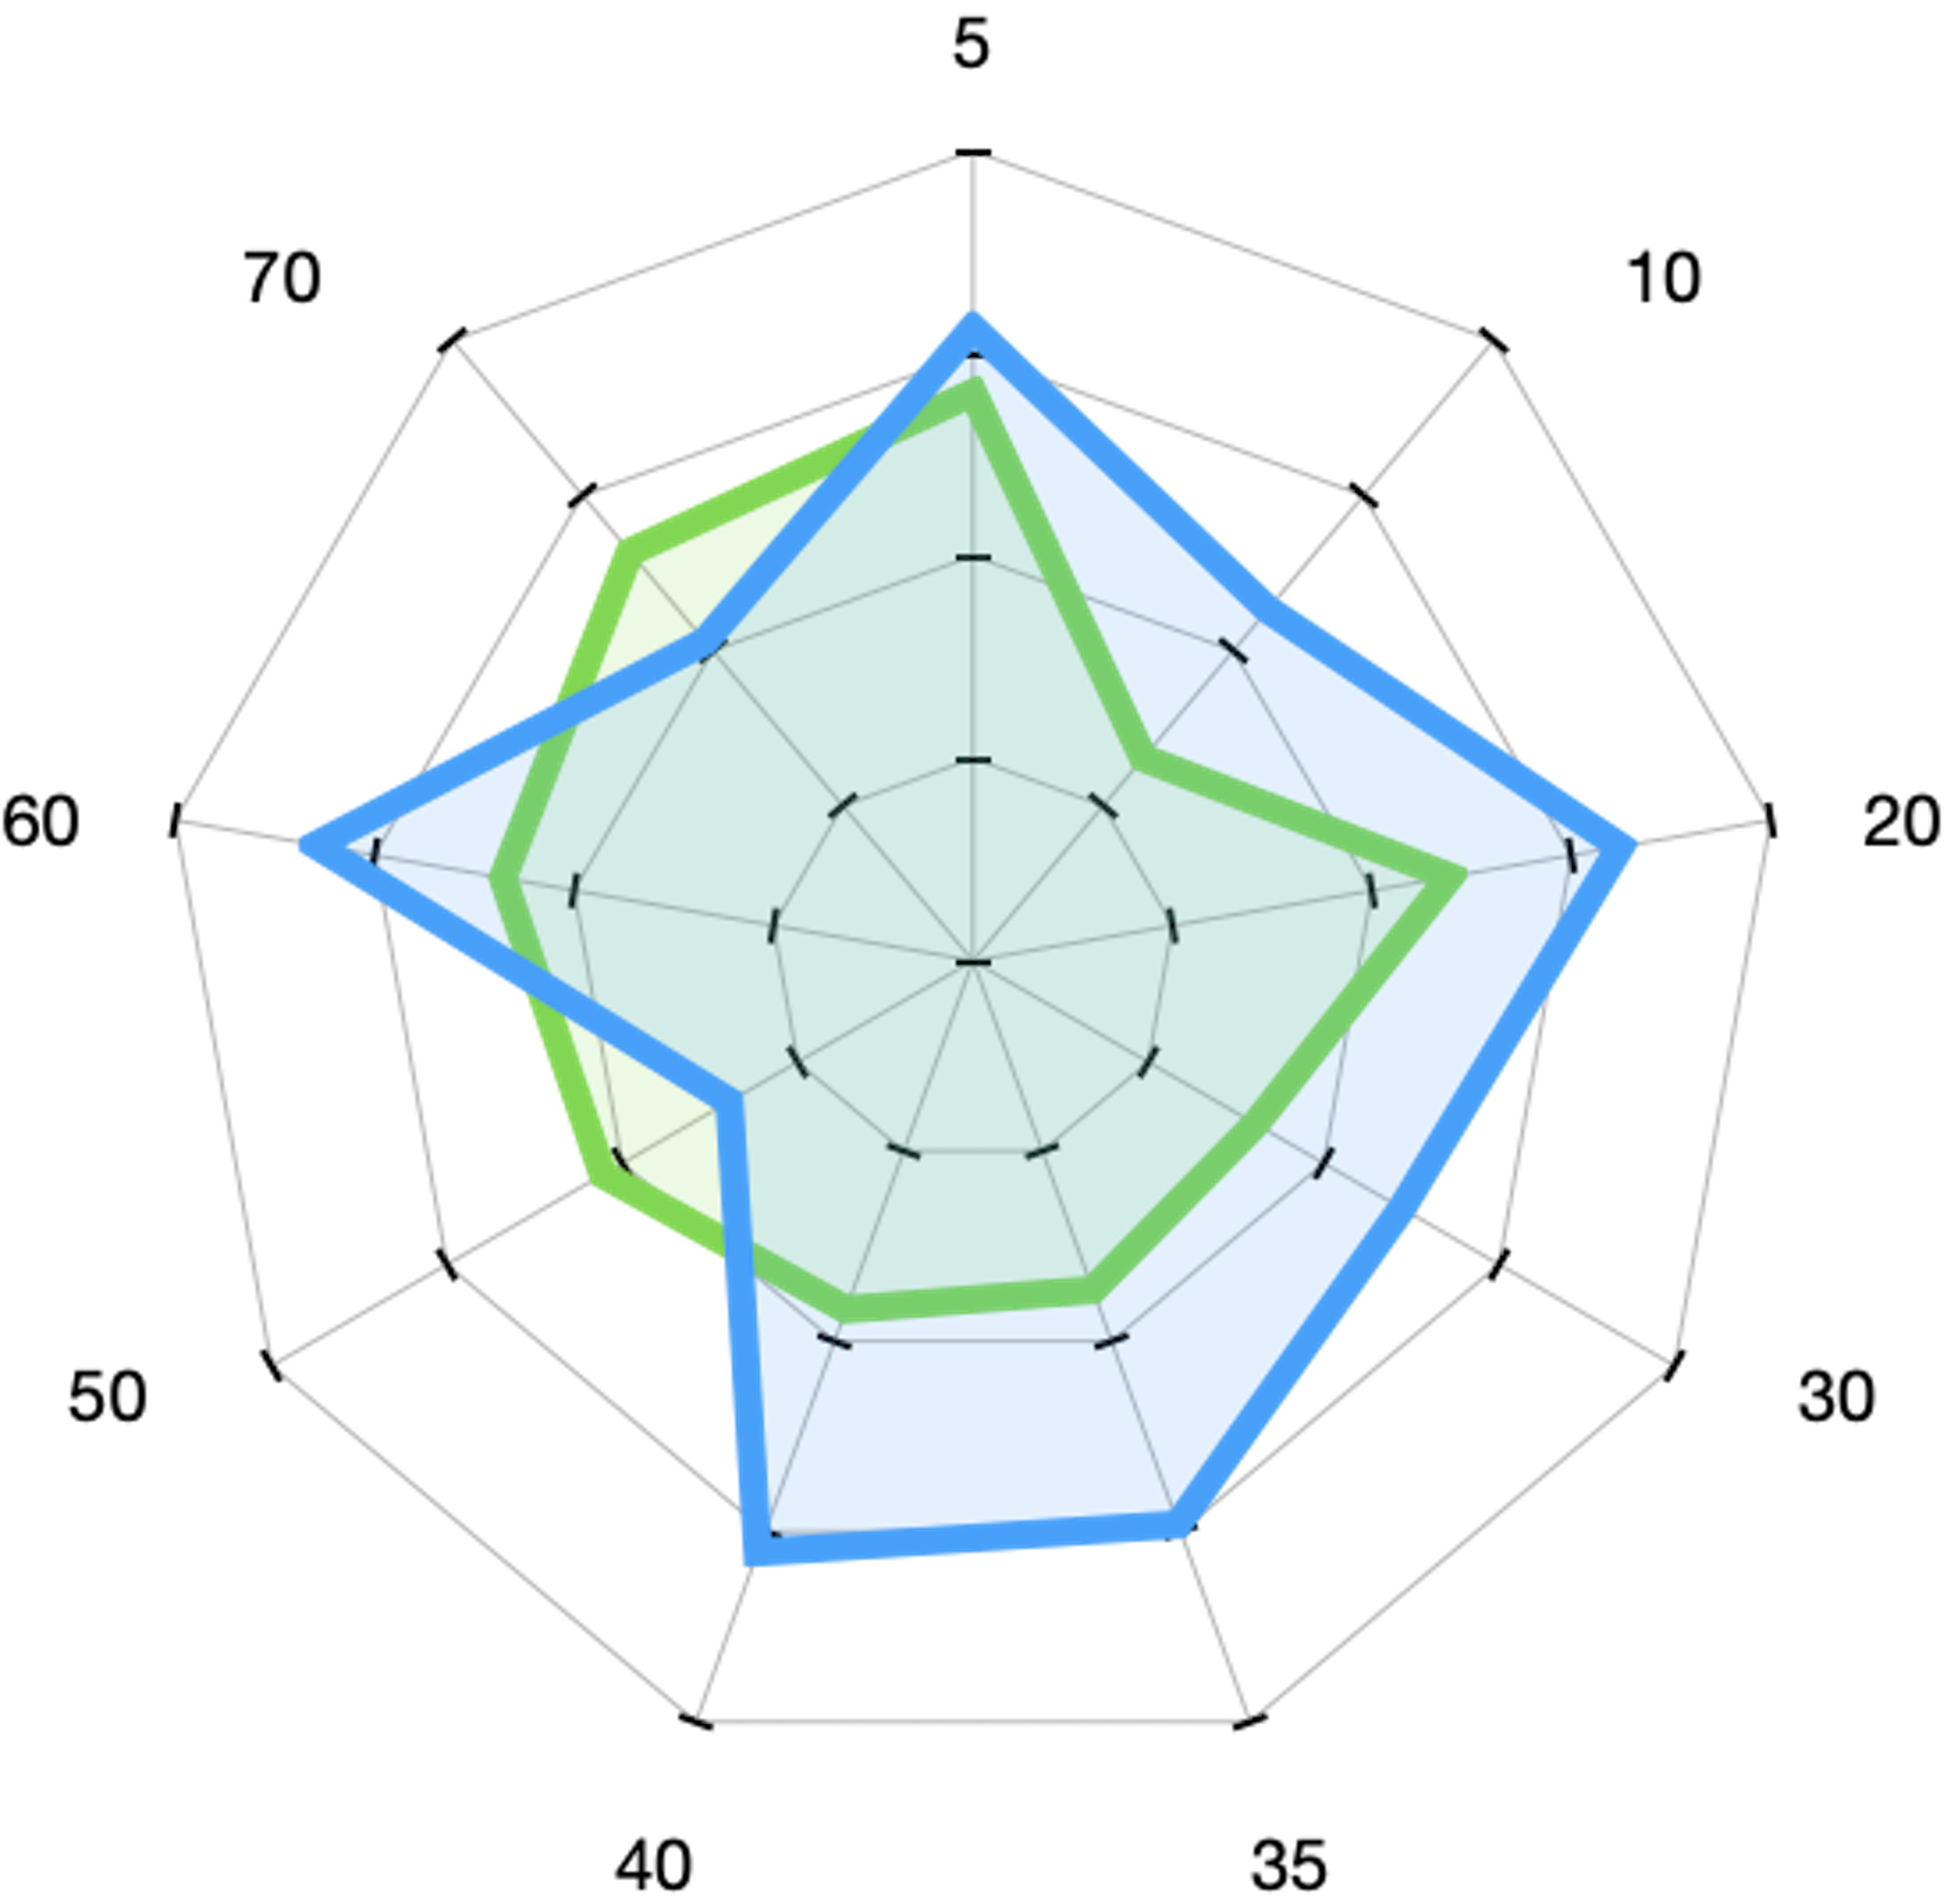
\includegraphics[width=0.4\textwidth, height=0.25\linewidth]{RNN_MAE_SPIDER.png}\label{fig:RNN_MAE_SPIDER}}\\
\subfloat[BiLSTM: UD-Batch ensemble Vs CUD ensemble]{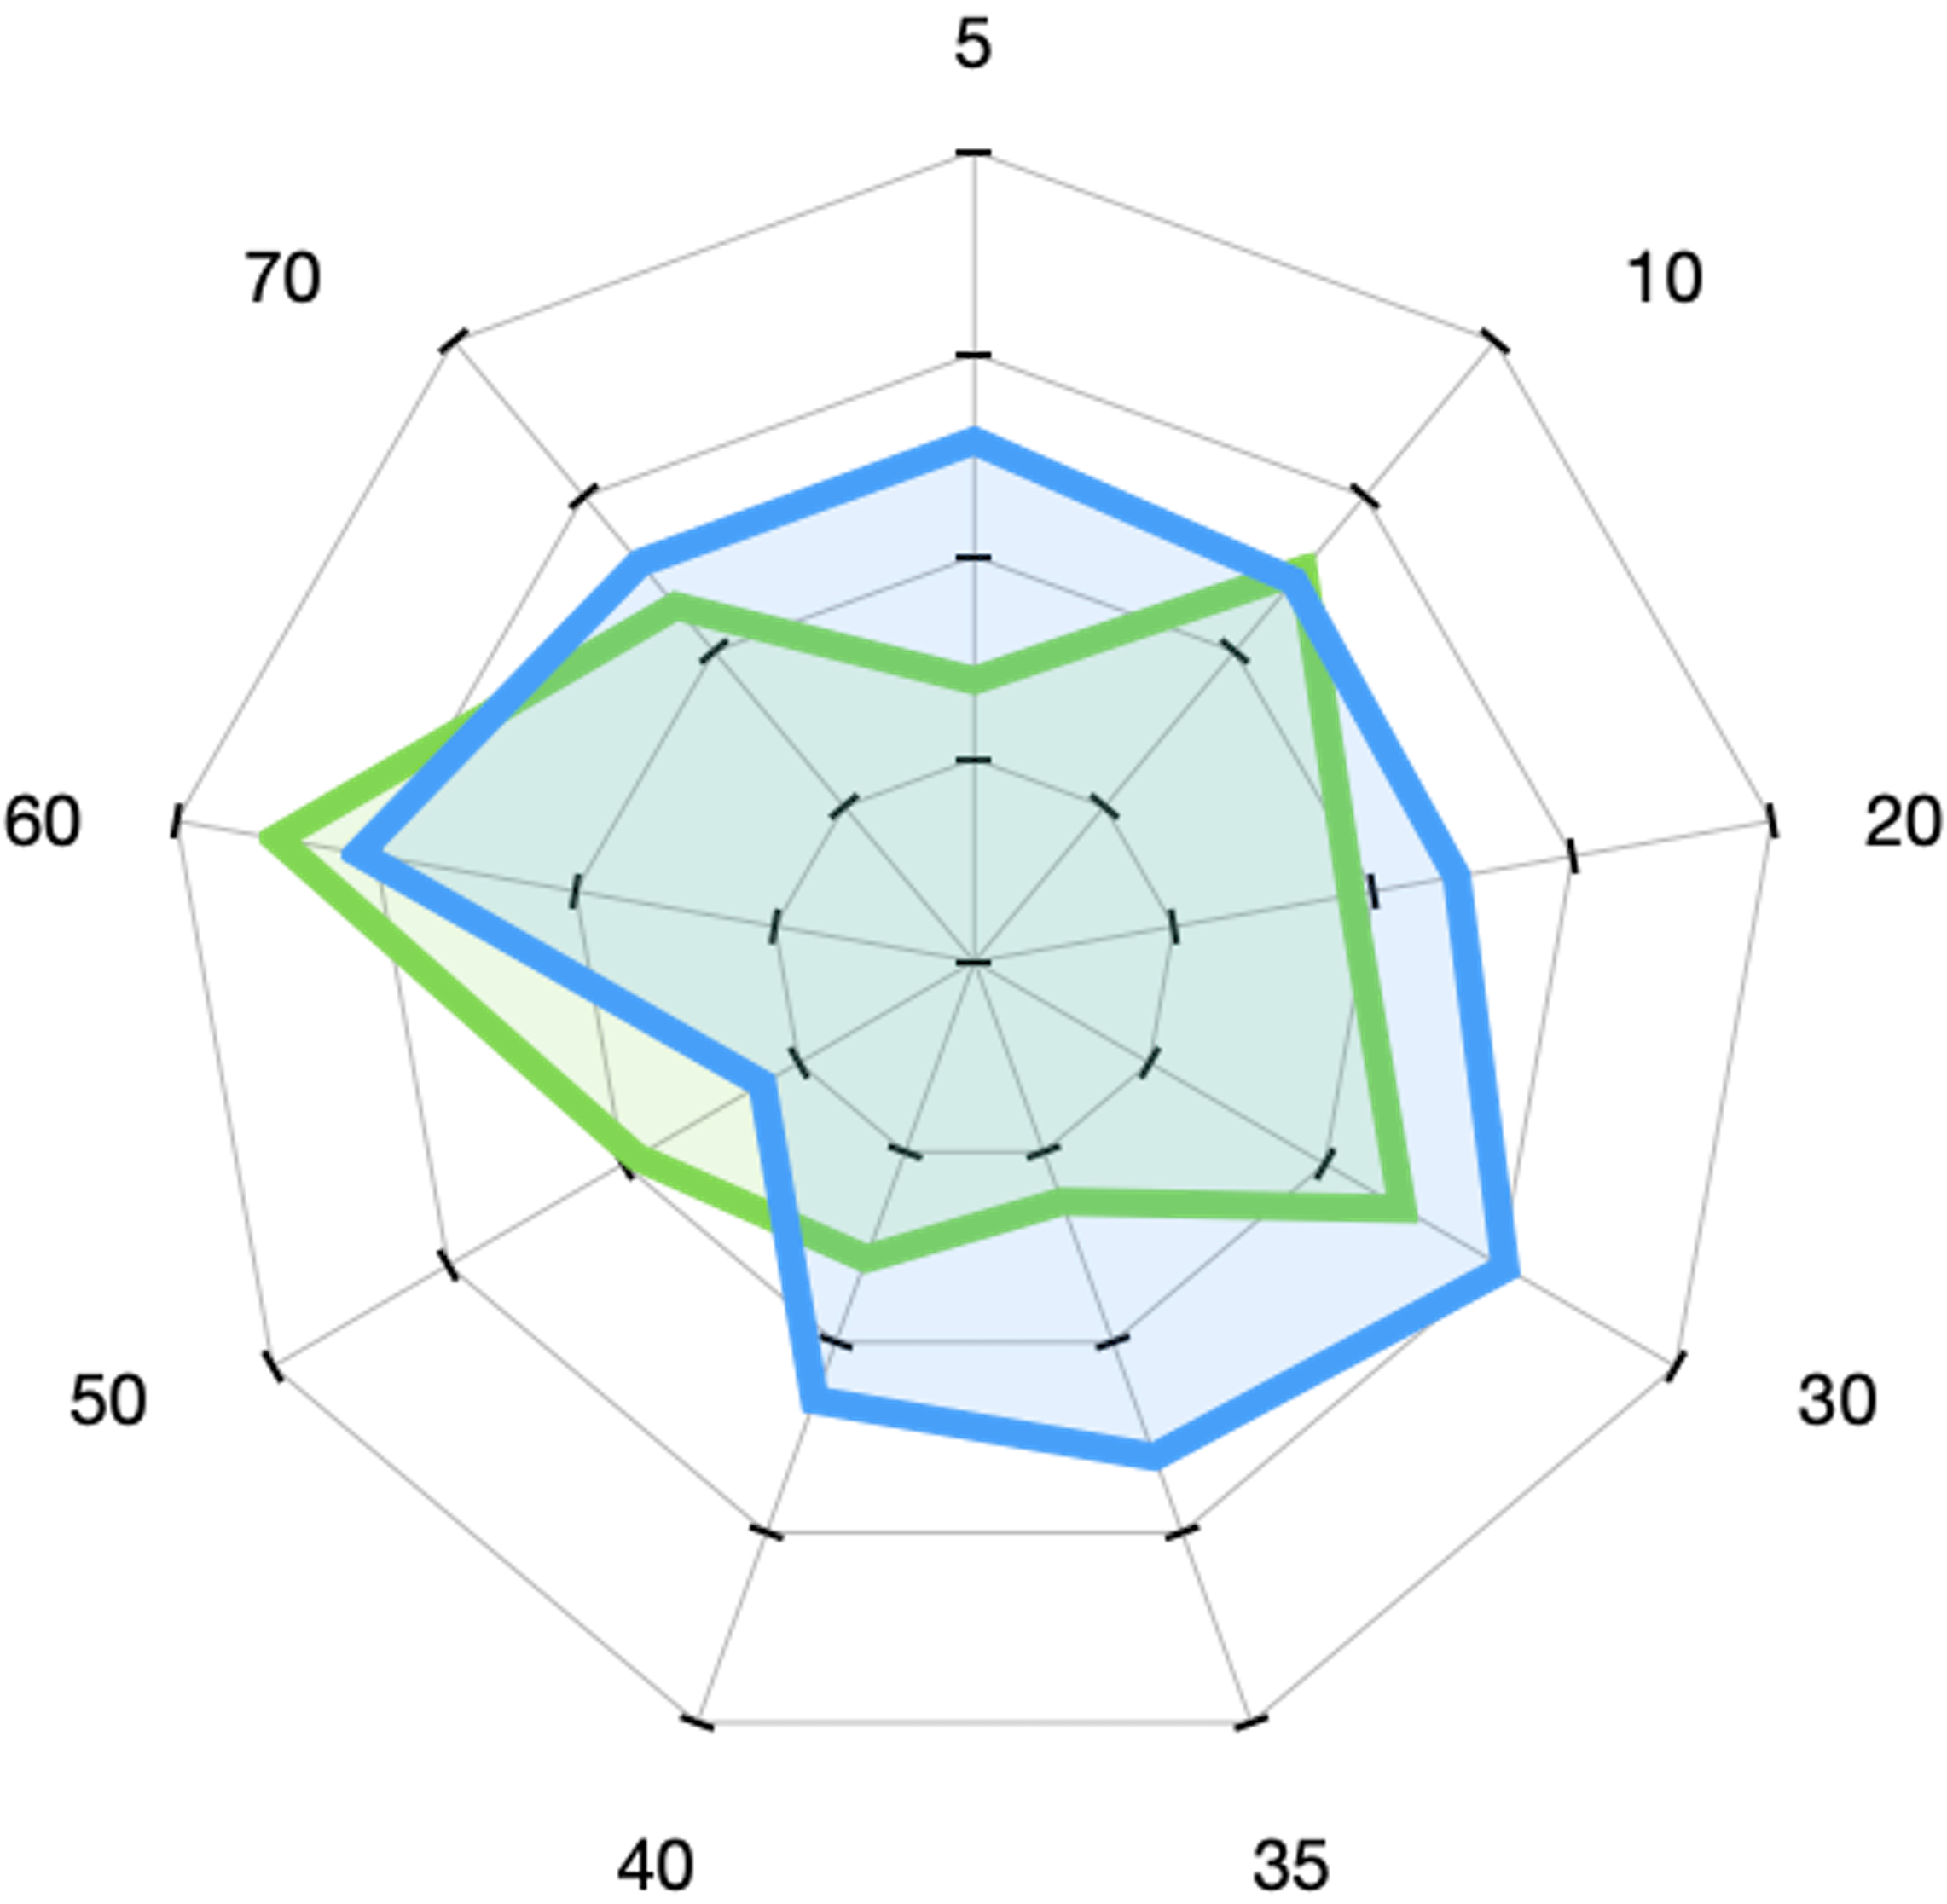
\includegraphics[width=0.4\textwidth, height=0.25\linewidth]{BI-LSTM_MAE_SPIDER.png}\label{fig:BiLSTM_MAE_SPIDER}}
\hfill
\subfloat[GRU: UD-Batch ensemble Vs CUD ensemble]{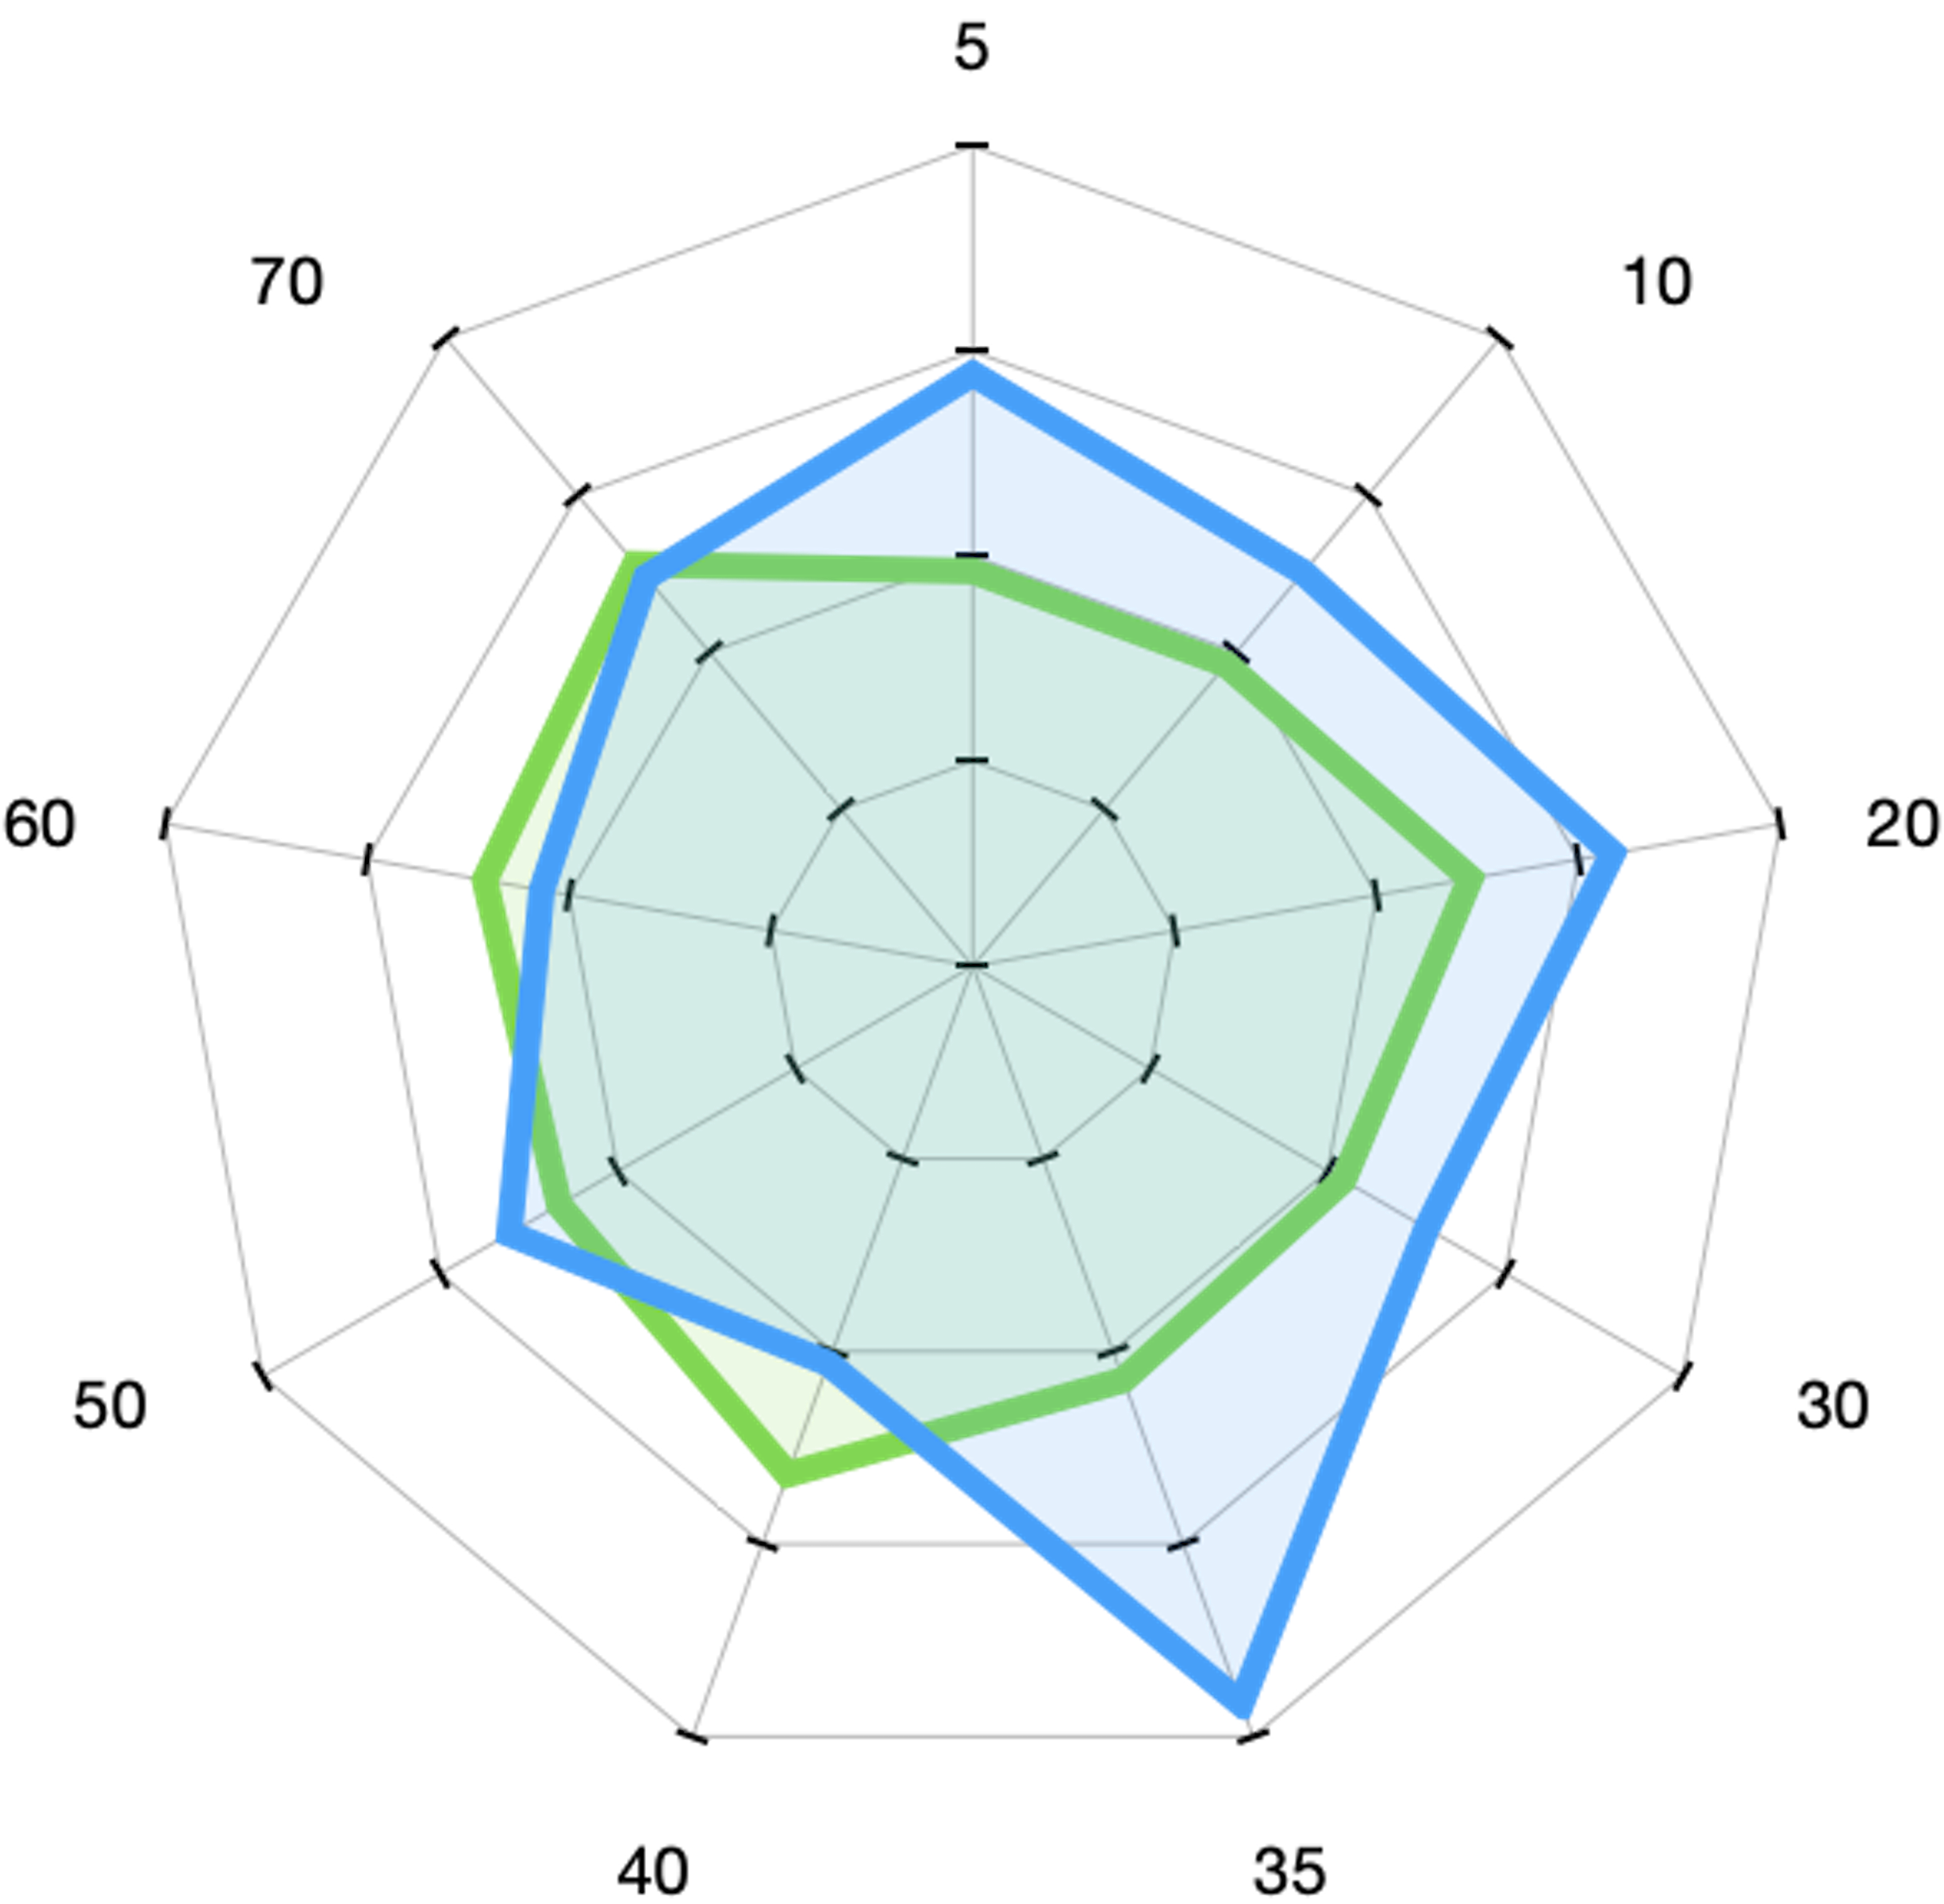
\includegraphics[width=0.4\textwidth, height=0.25\linewidth]{GRU_MAE_SPIDER.png}\label{fig:GRU_MAE_SPIDER}}
\caption{comparison of models over MAE}
\label{fig:all_models_mae}
\end{figure}
\begin{figure}[ht!]
%\centering
\subfloat[LSTM: UD-Batch ensemble Vs CUD ensemble]{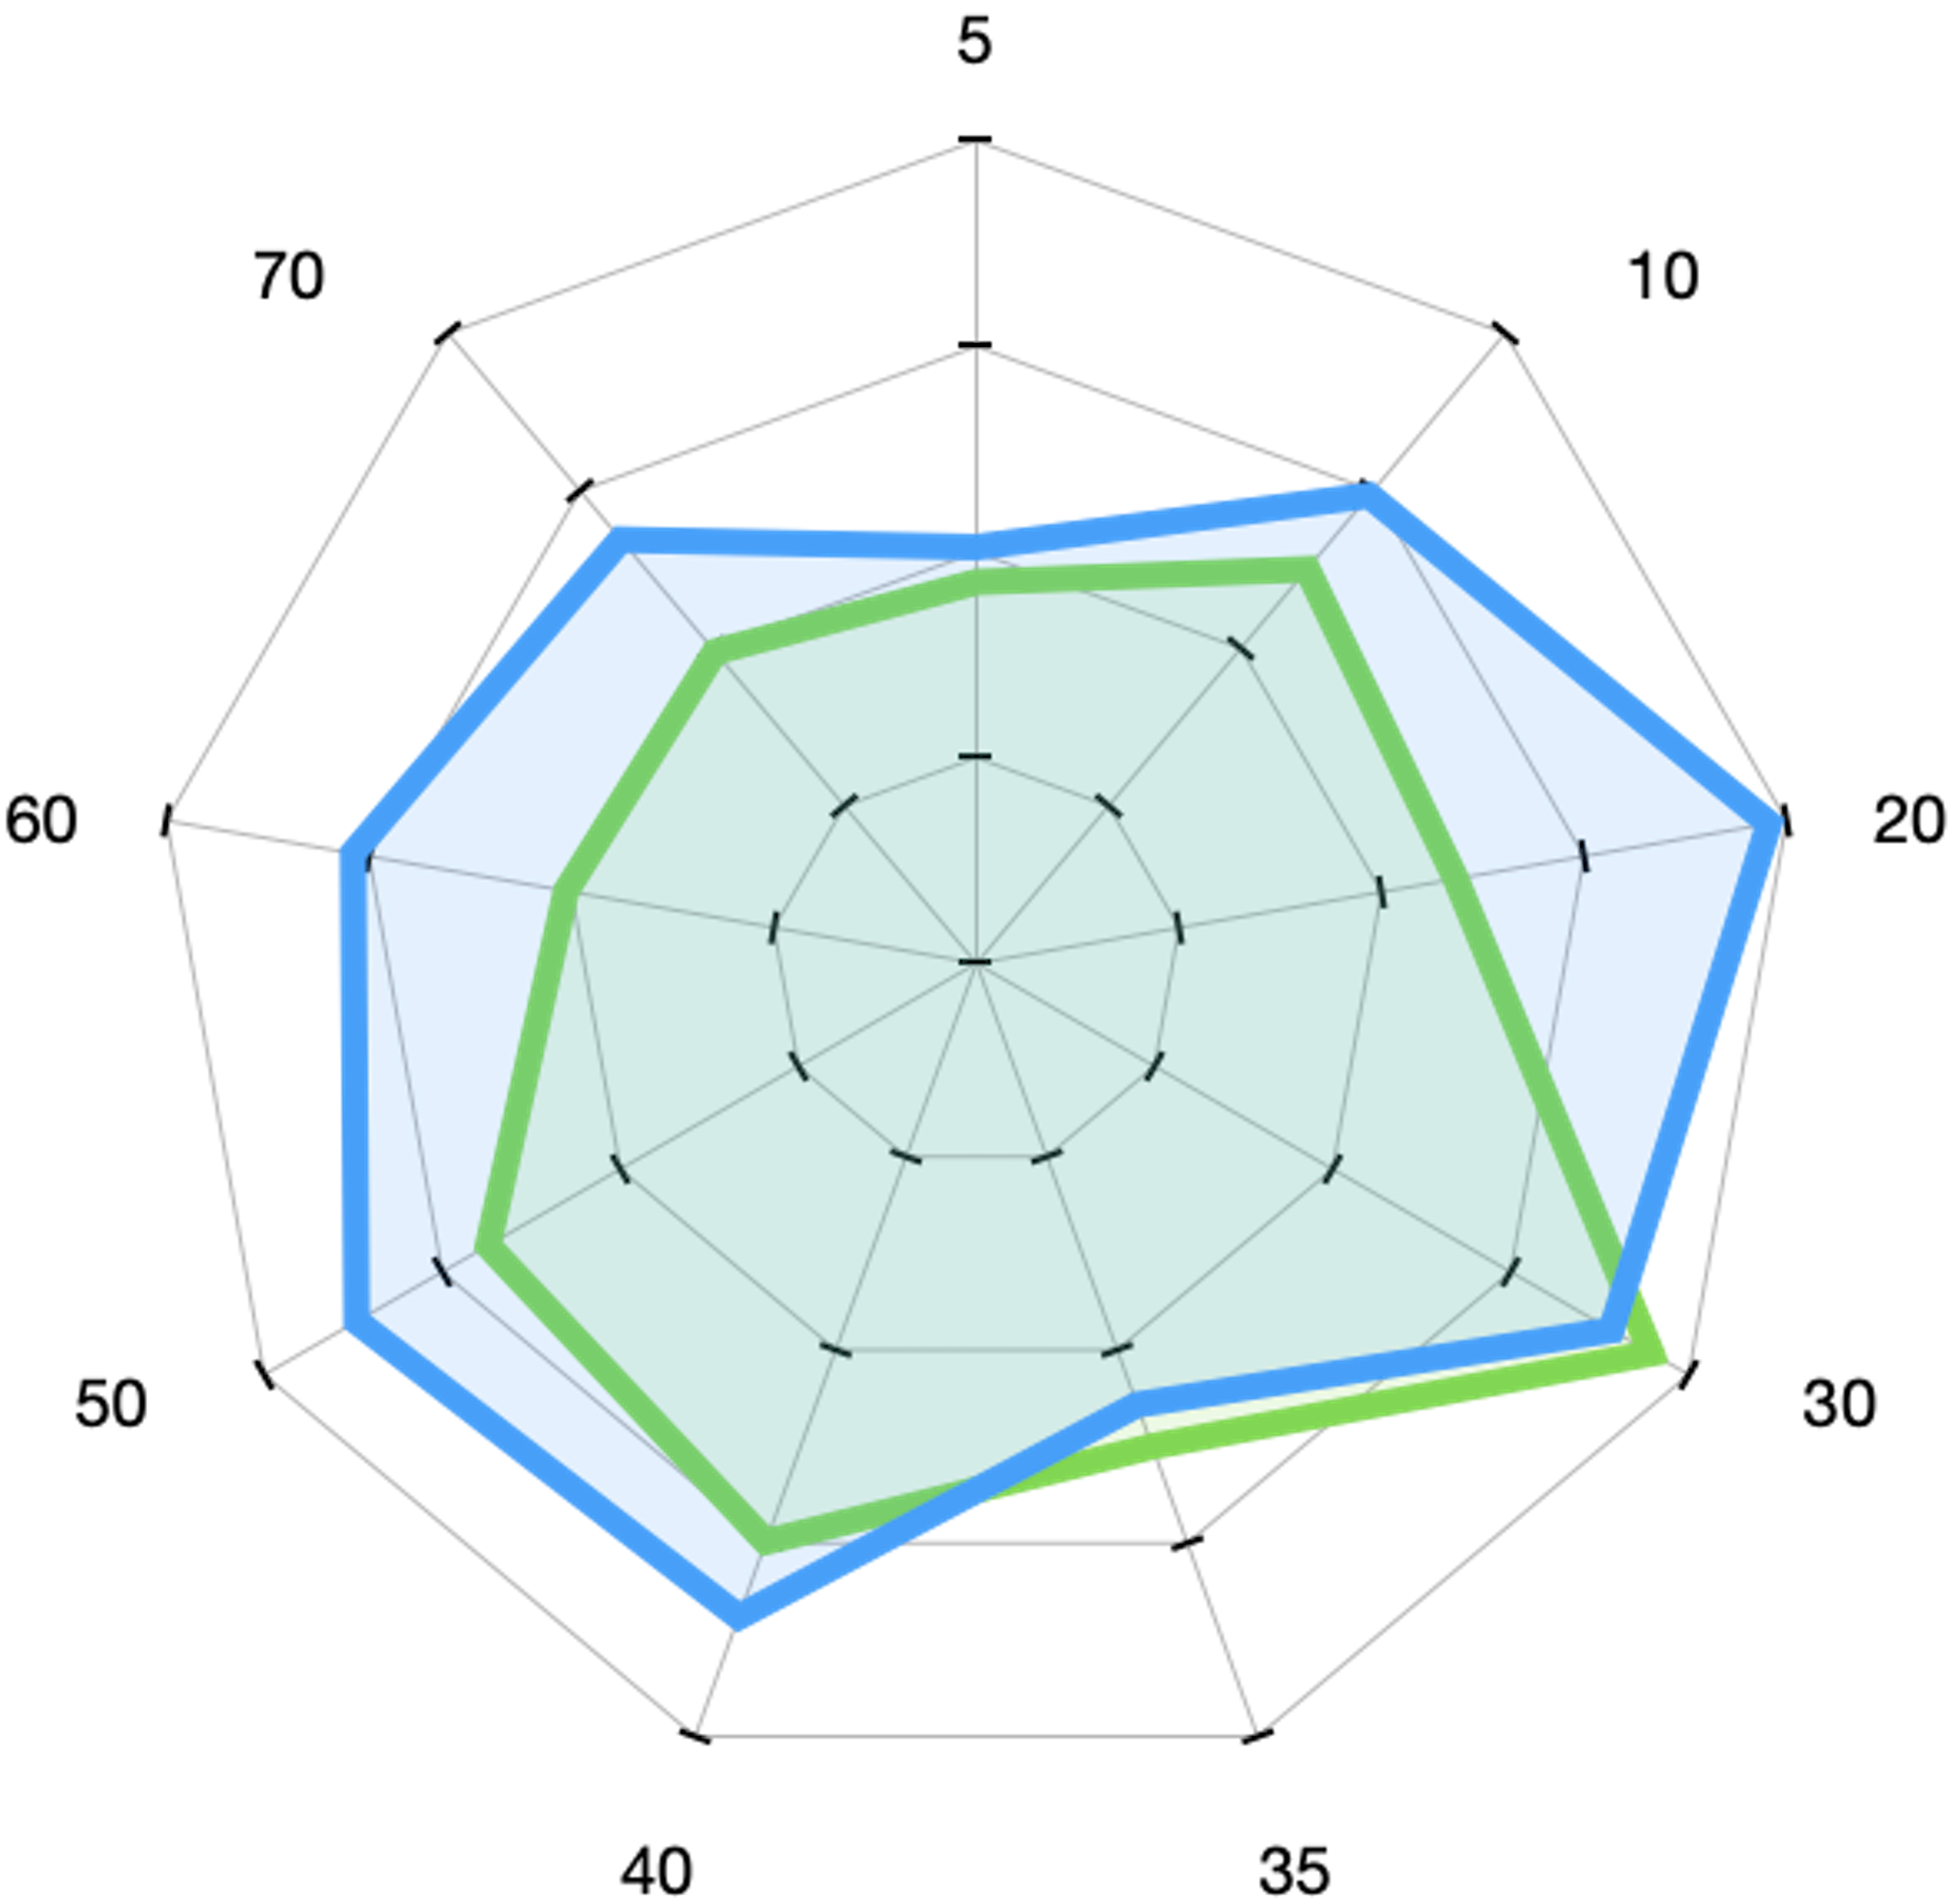
\includegraphics[width=0.4\textwidth, height=0.25\linewidth]{LSTM_MSE_SPIDER.png}\label{fig:LSTM MSE SPIDER}}
\hfill
\subfloat[RNN: UD-Batch ensemble Vs CUD ensemble]{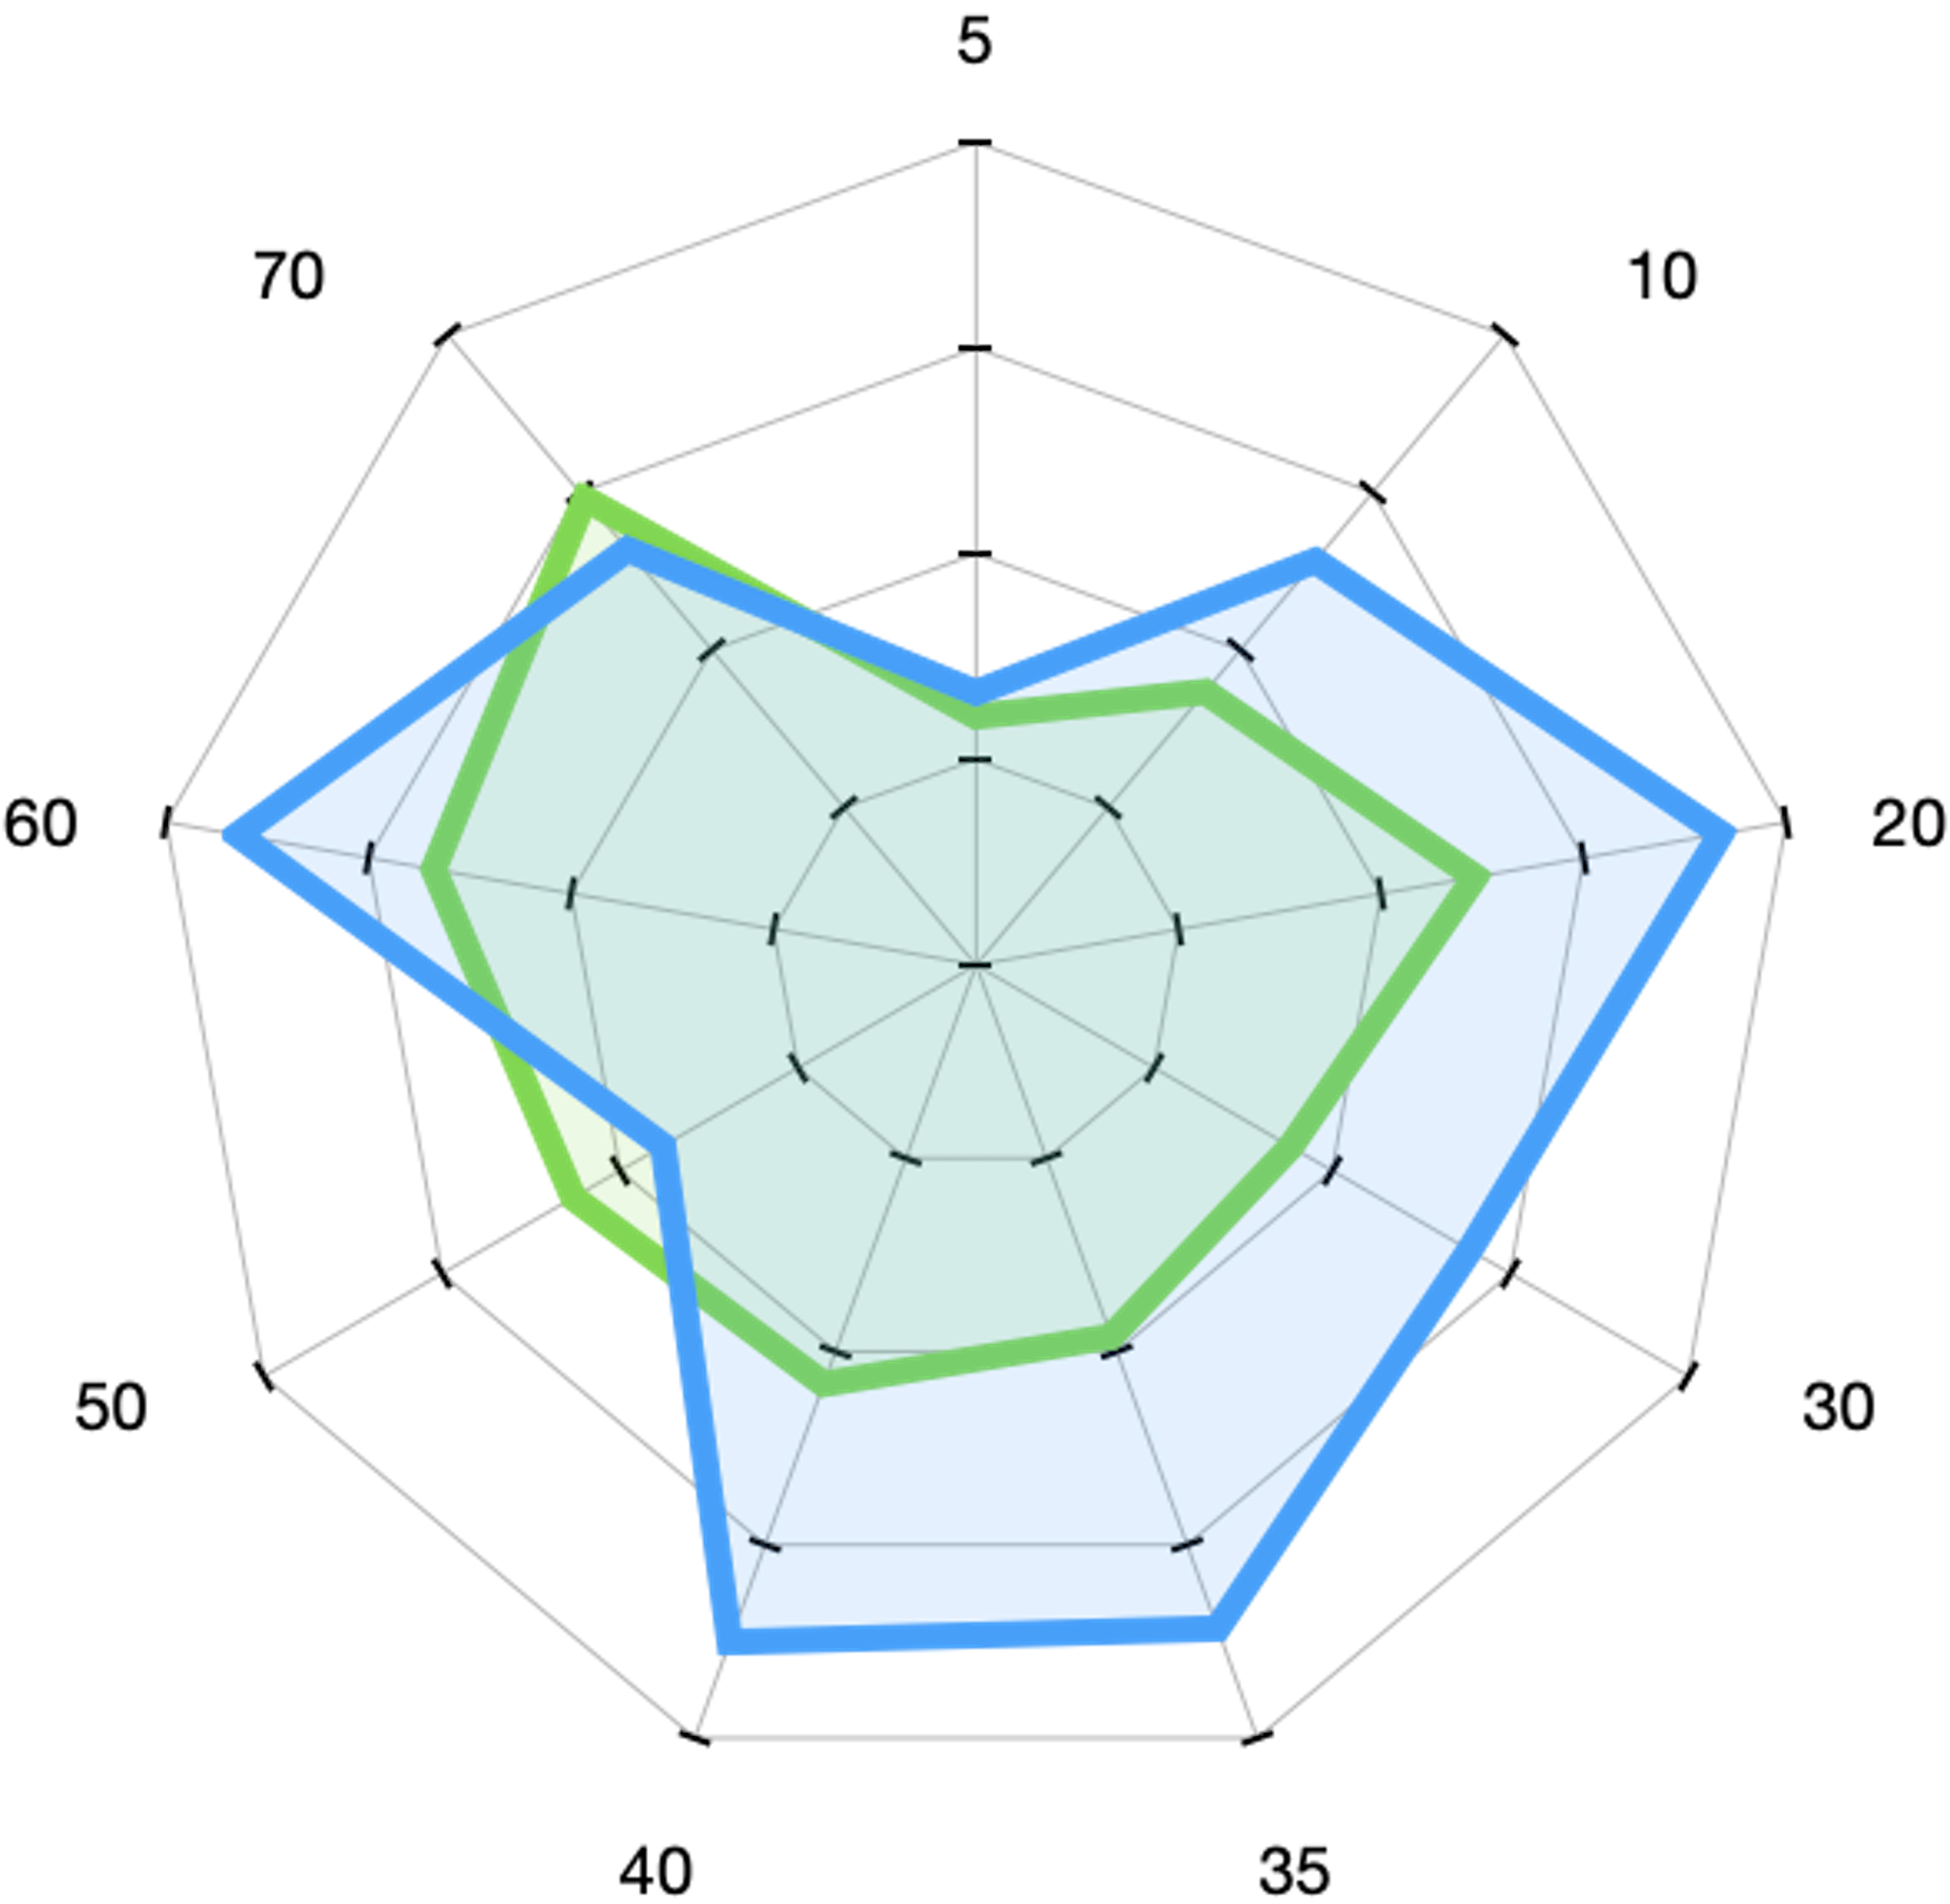
\includegraphics[width=0.4\textwidth, height=0.25\linewidth]{RNN_MSE_SPIDER.png}\label{fig:RNN_MSE_SPIDER}}
% \vspace{\baselineskip} % Add vertical space between rows
\\
\subfloat[BiLSTM: UD-Batch ensemble Vs CUD ensemble]{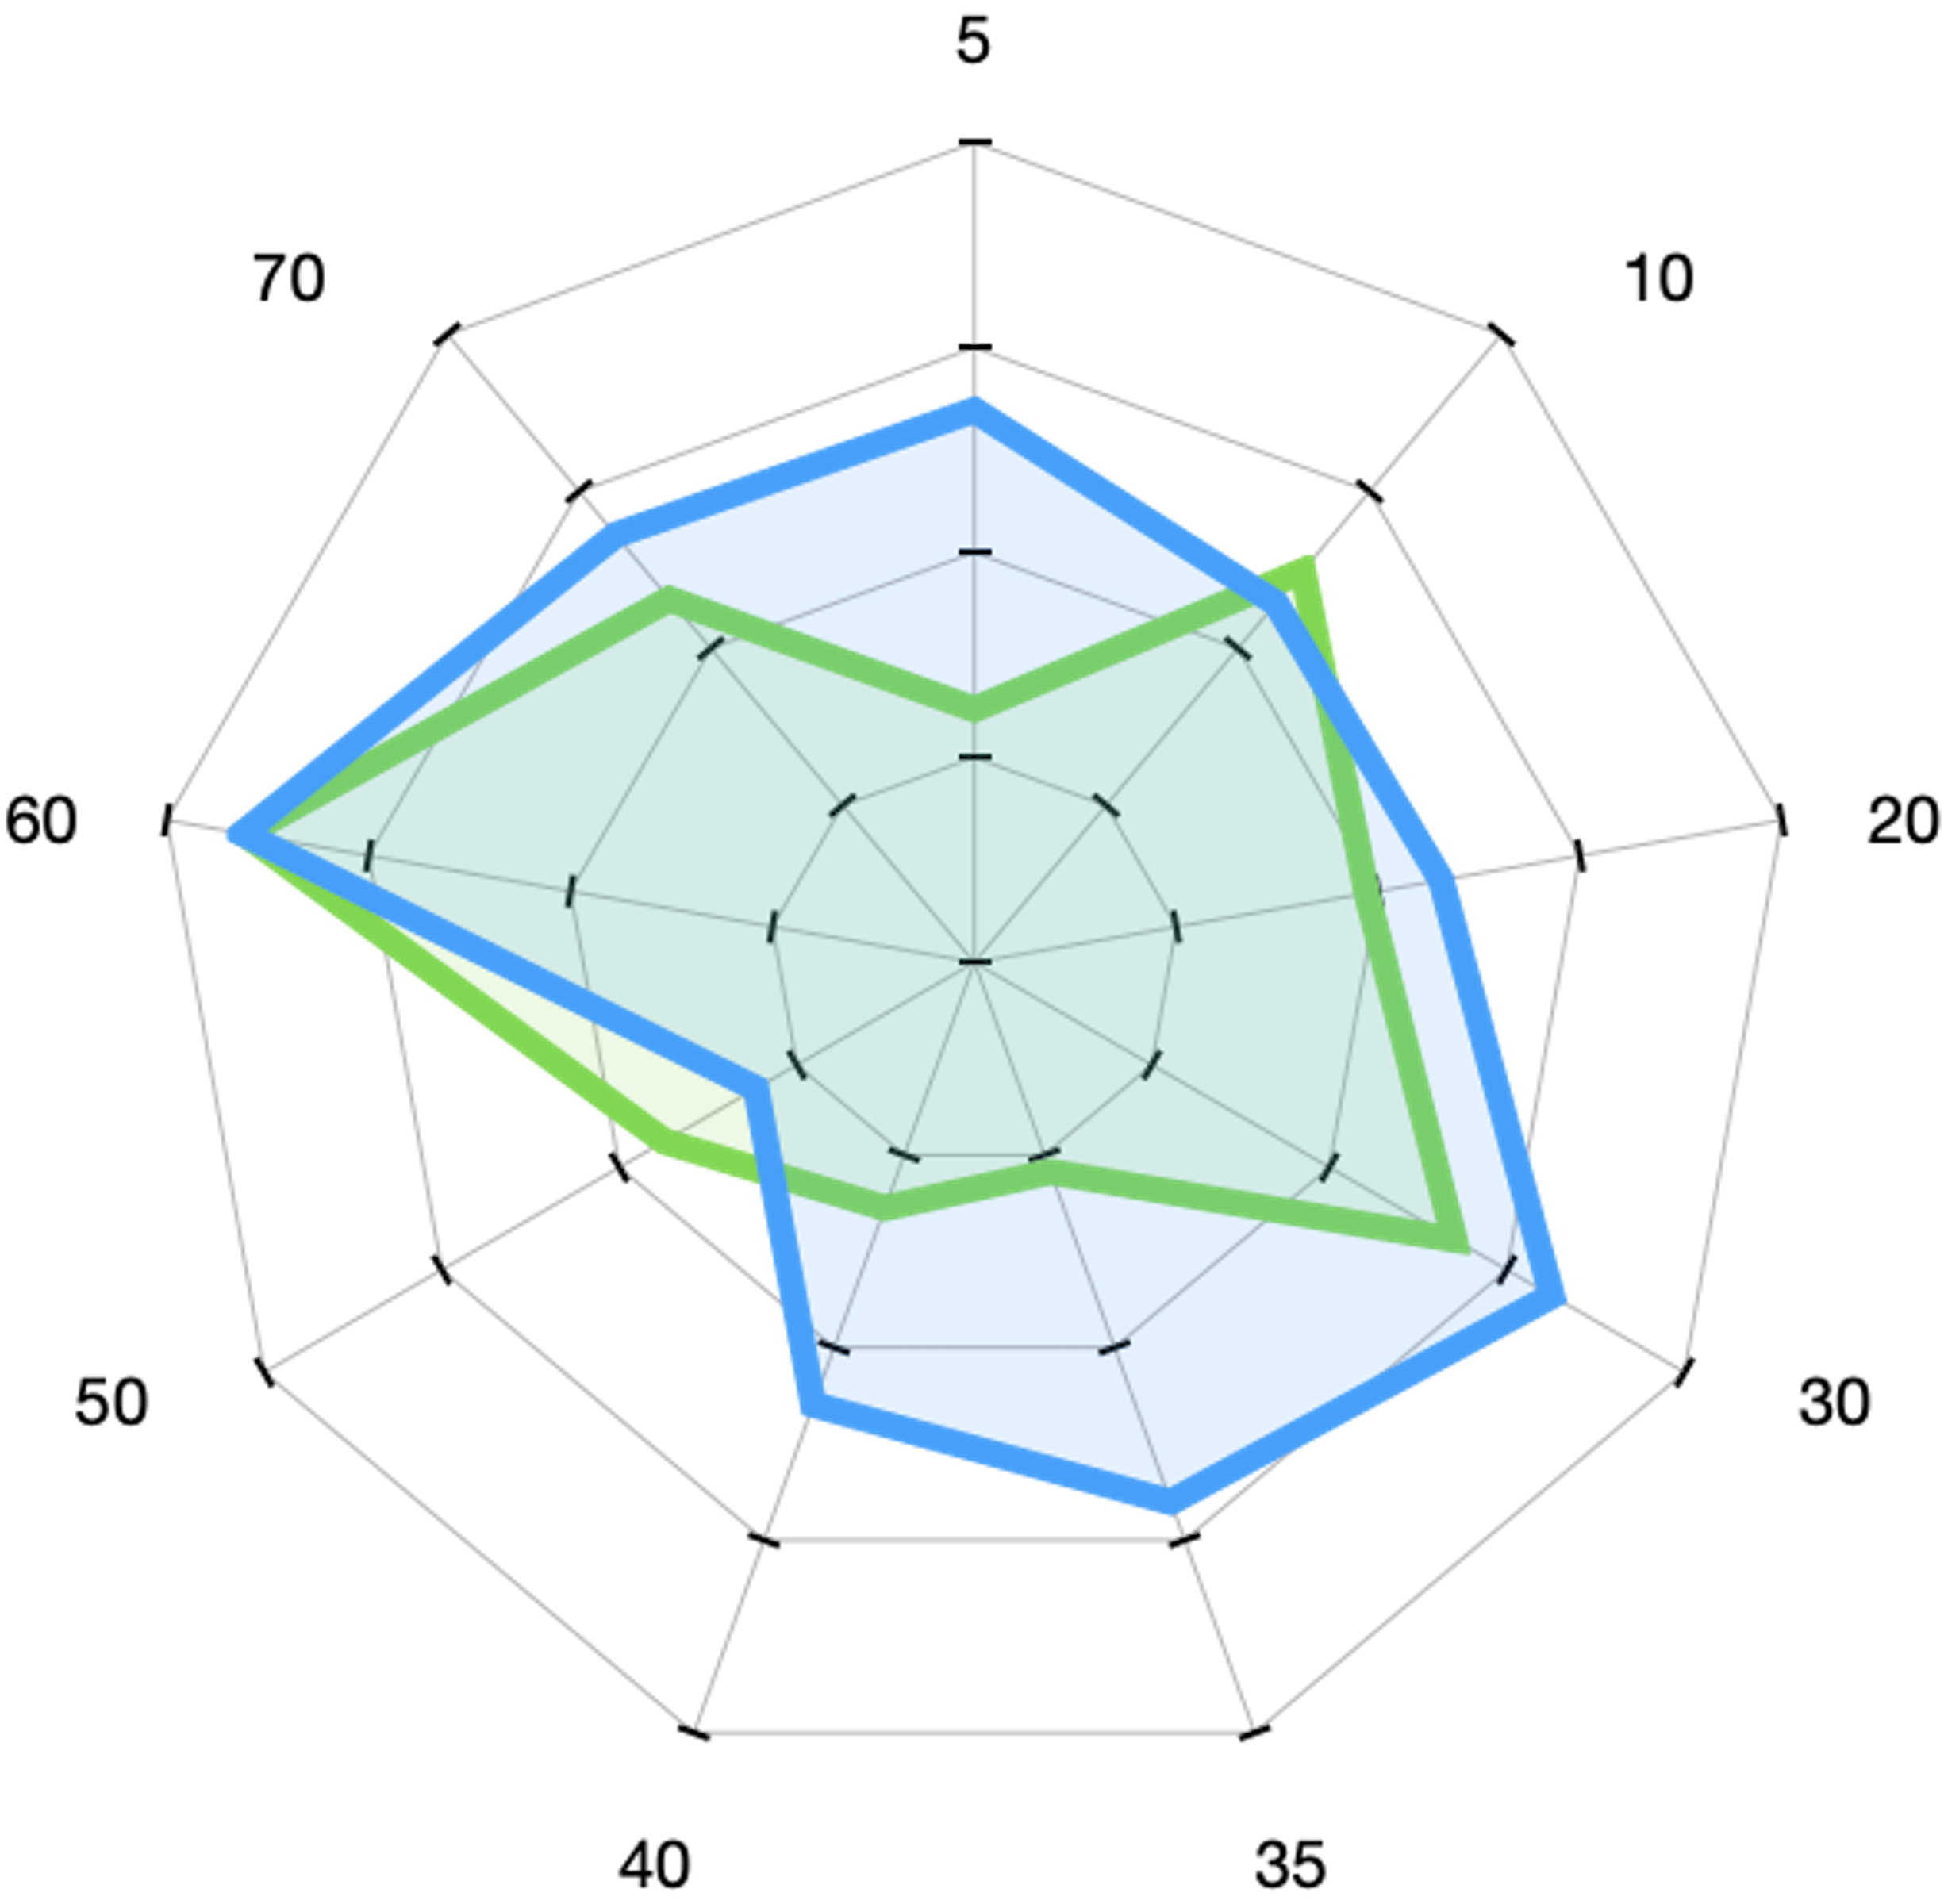
\includegraphics[width=0.4\textwidth, height=0.25\linewidth]{BI-LSTM_MSE_SPIDER.png}\label{fig:BiLSTM_MSE_SPIDER}}
\hfill
\subfloat[GRU: UD-Batch ensemble Vs CUD ensemble]{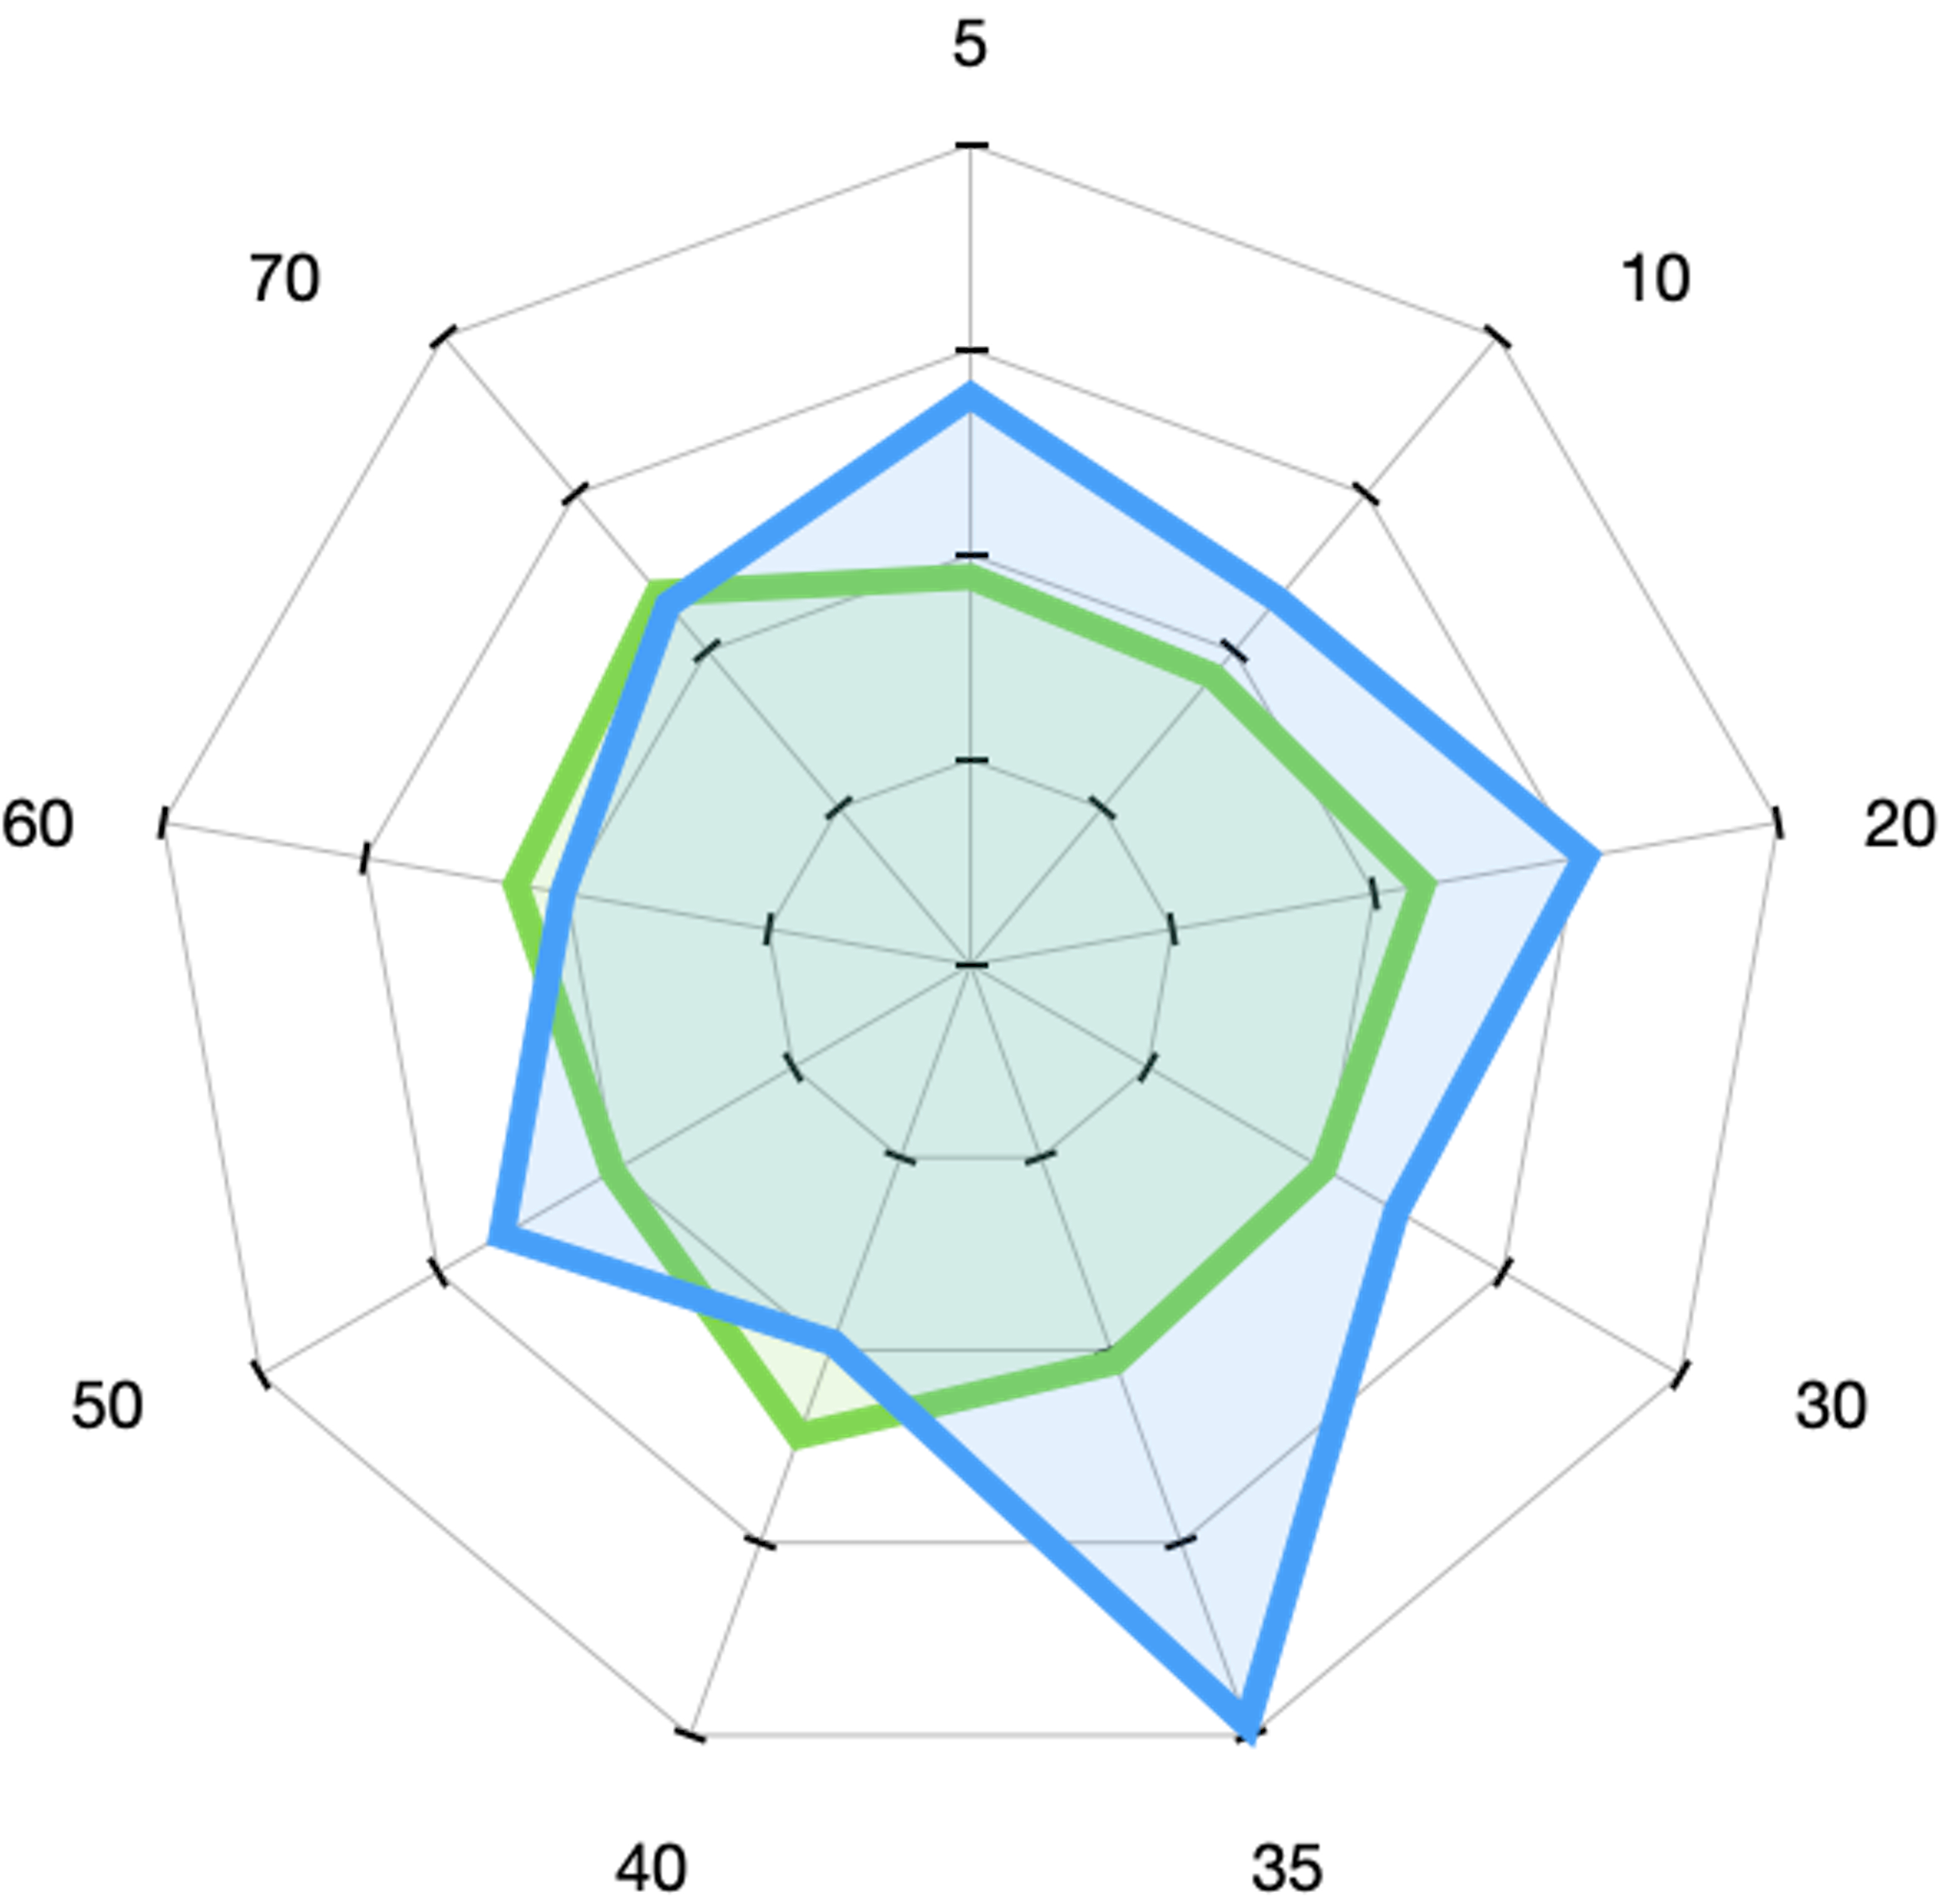
\includegraphics[width=0.4\textwidth, height=0.25\linewidth]{GRU_MSE_SPIDER.png}\label{fig:GRU_MSE_SPIDER}}
\caption{Performance comparison of Upward batch and Downward batch ensemble(UD-Batch) and Corresponding upward and downward ensemble(CUD-ensemble) using DL models over MAE performance measure.}
\label{fig:all_models_mse}
\end{figure}


\begin{figure}[ht!]
%\centering
\subfloat[LSTM: UD-Batch ensemble Vs CUD ensemble]{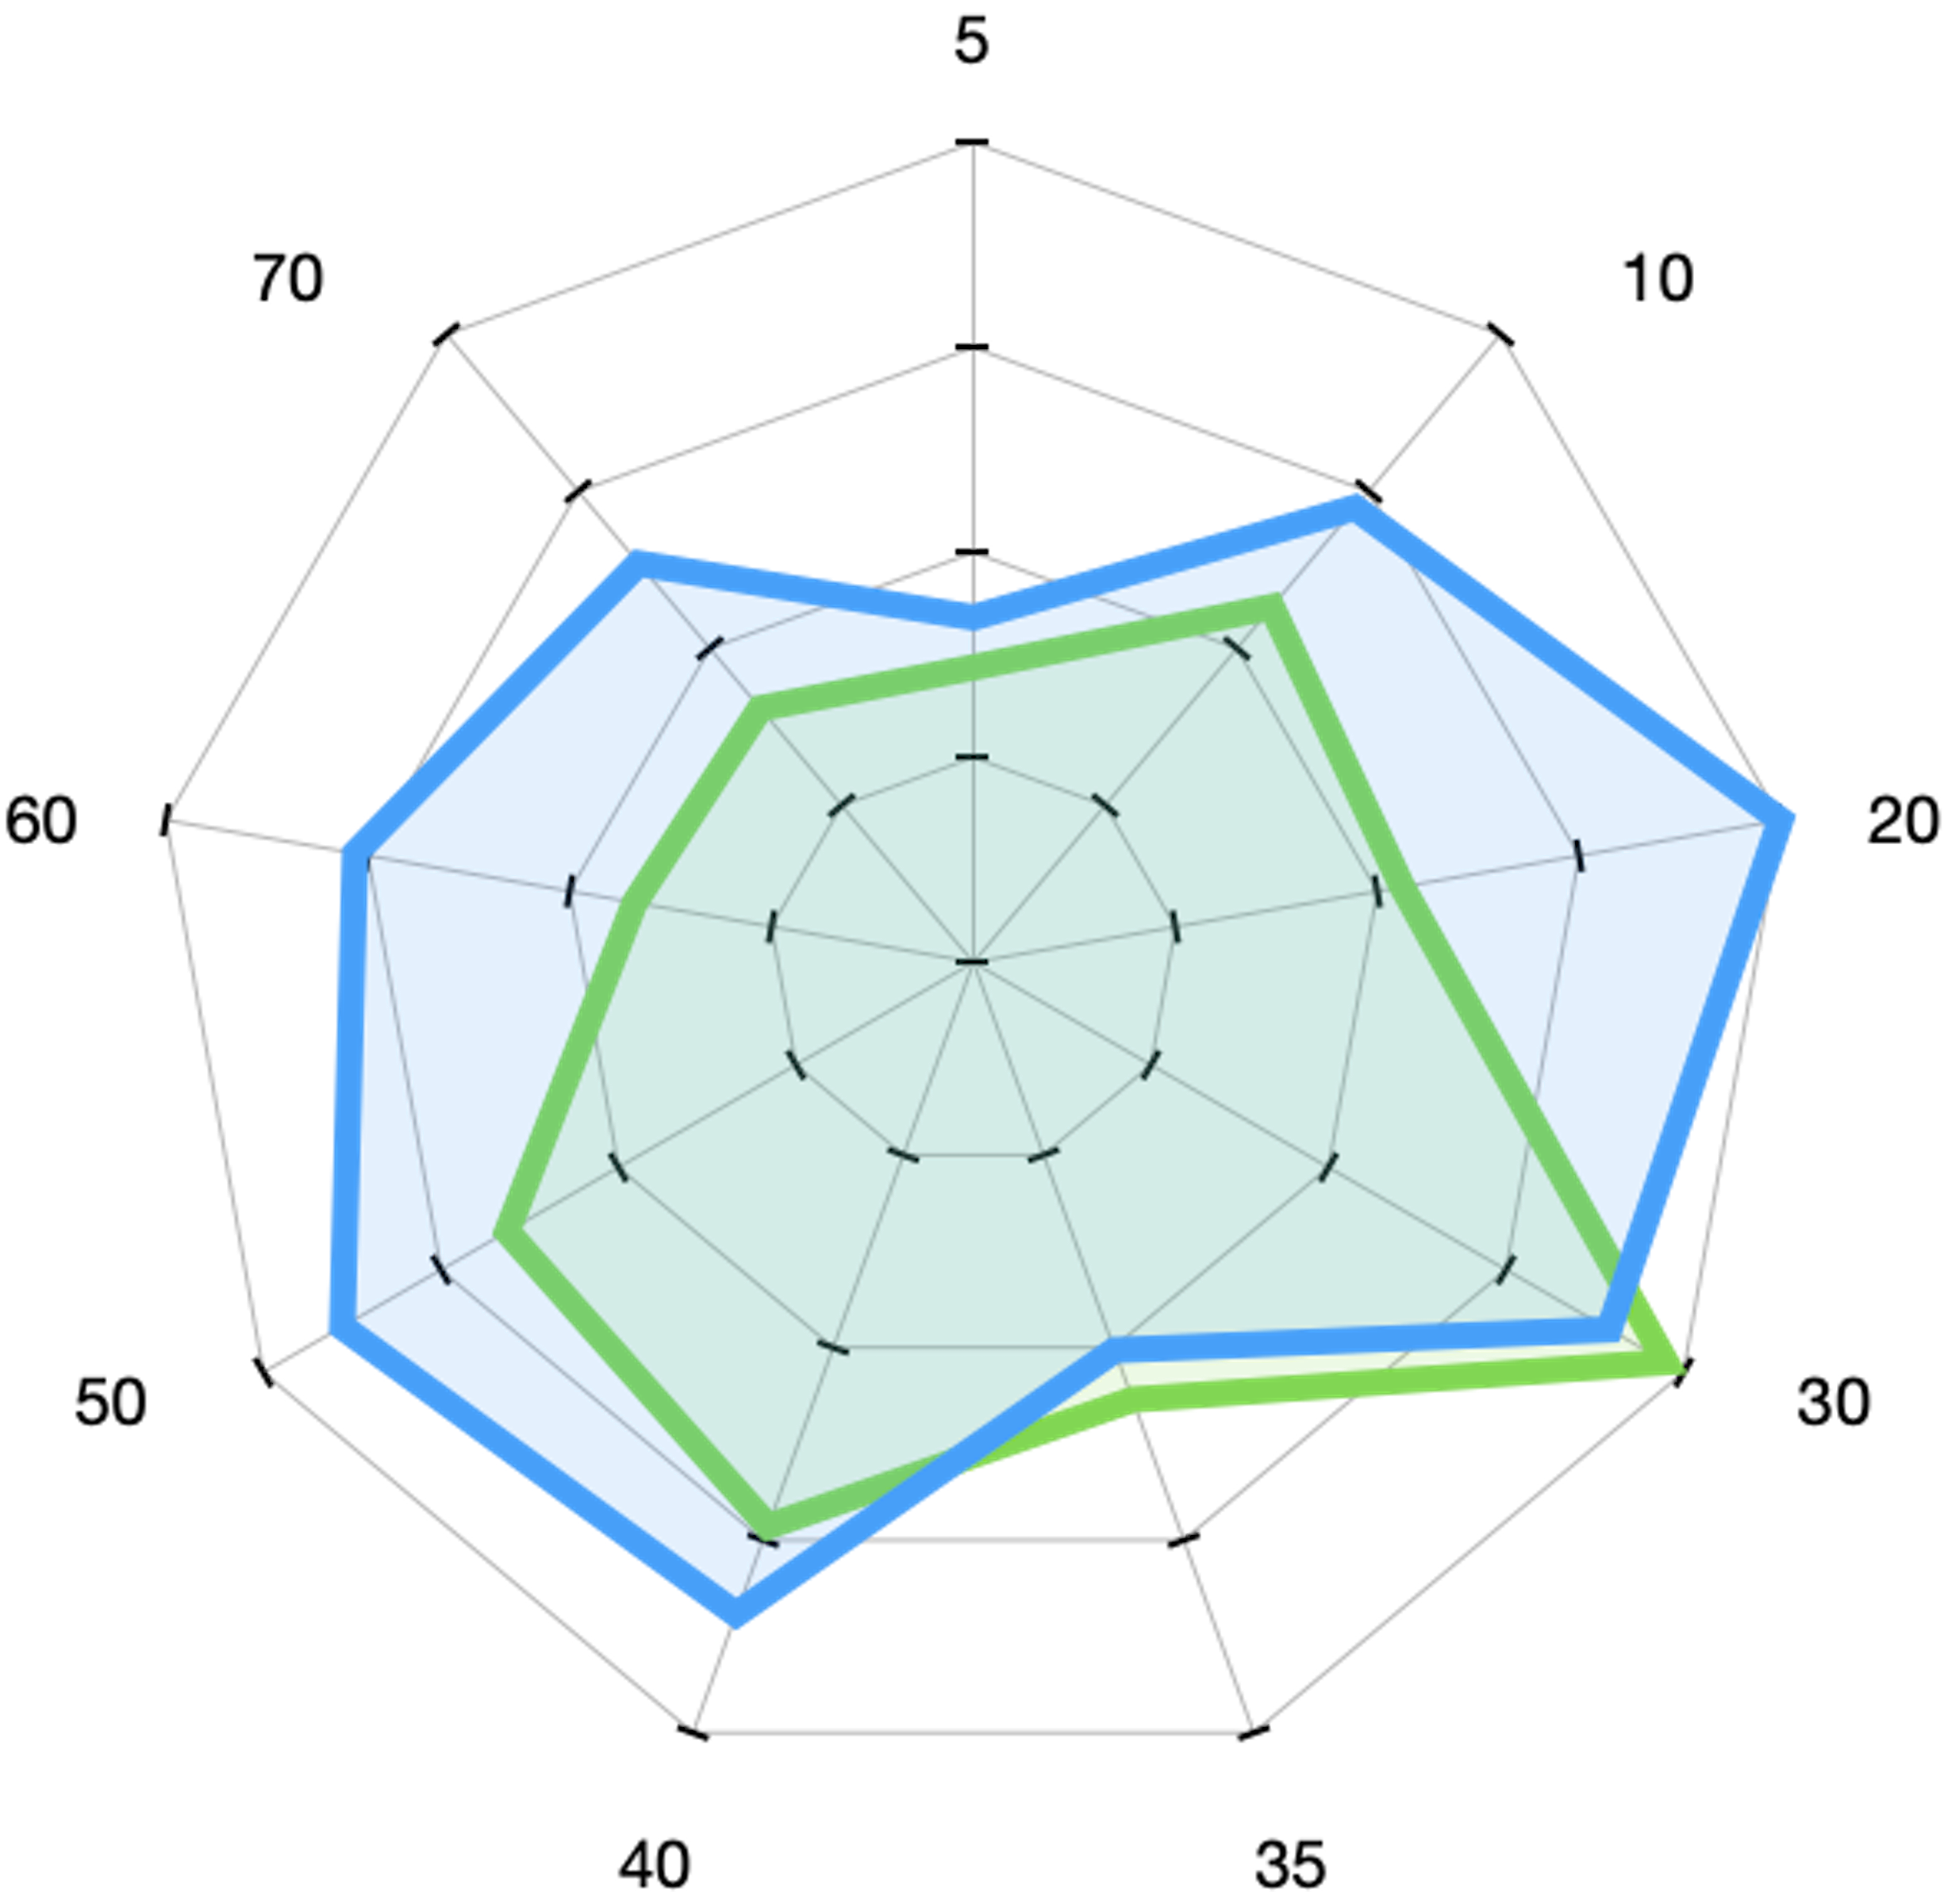
\includegraphics[width=0.4\textwidth, height=0.25\linewidth]{LSTM_RMSE_SPIDER.png}\label{fig:LSTM RMSE SPIDER}}
\hfill
\subfloat[RNN: UD-Batch ensemble Vs CUD ensemble]{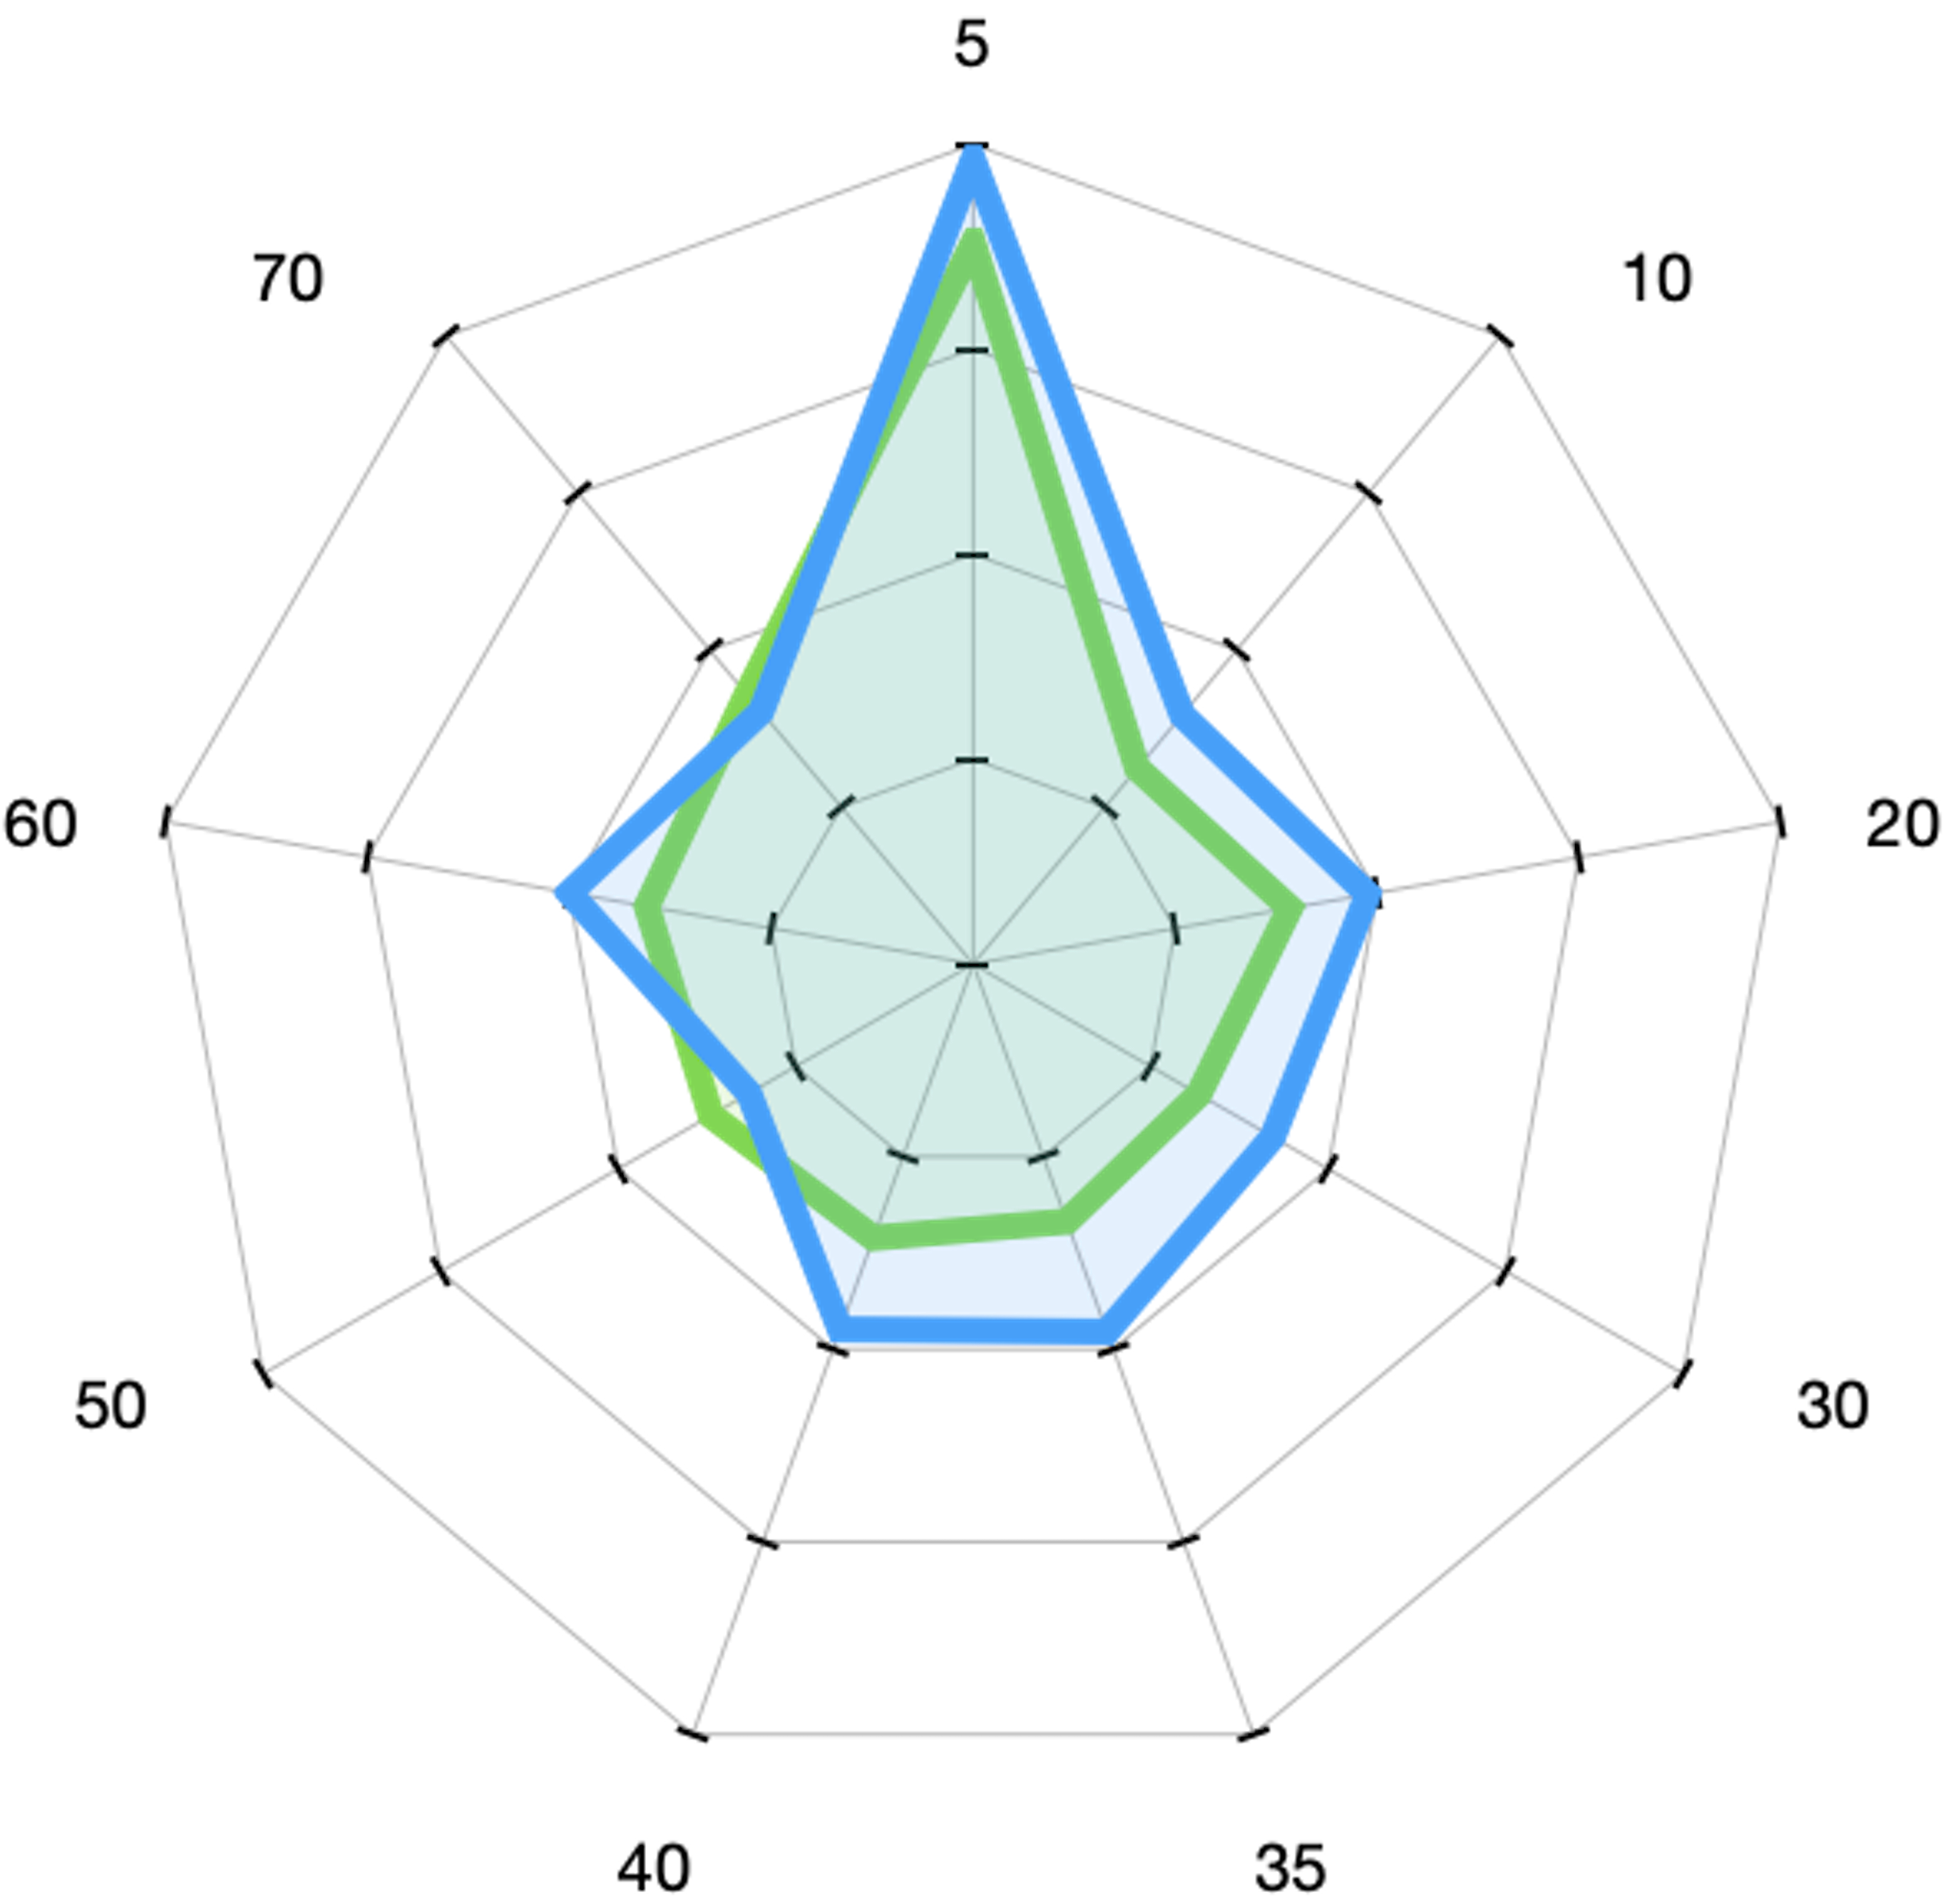
\includegraphics[width=0.4\textwidth, height=0.25\linewidth]{RNN_RMSE_SPIDER.png}\label{fig:RNN_RMSE_SPIDER}}
\\
\subfloat[BiLSTM: UD-Batch ensemble Vs CUD ensemble]{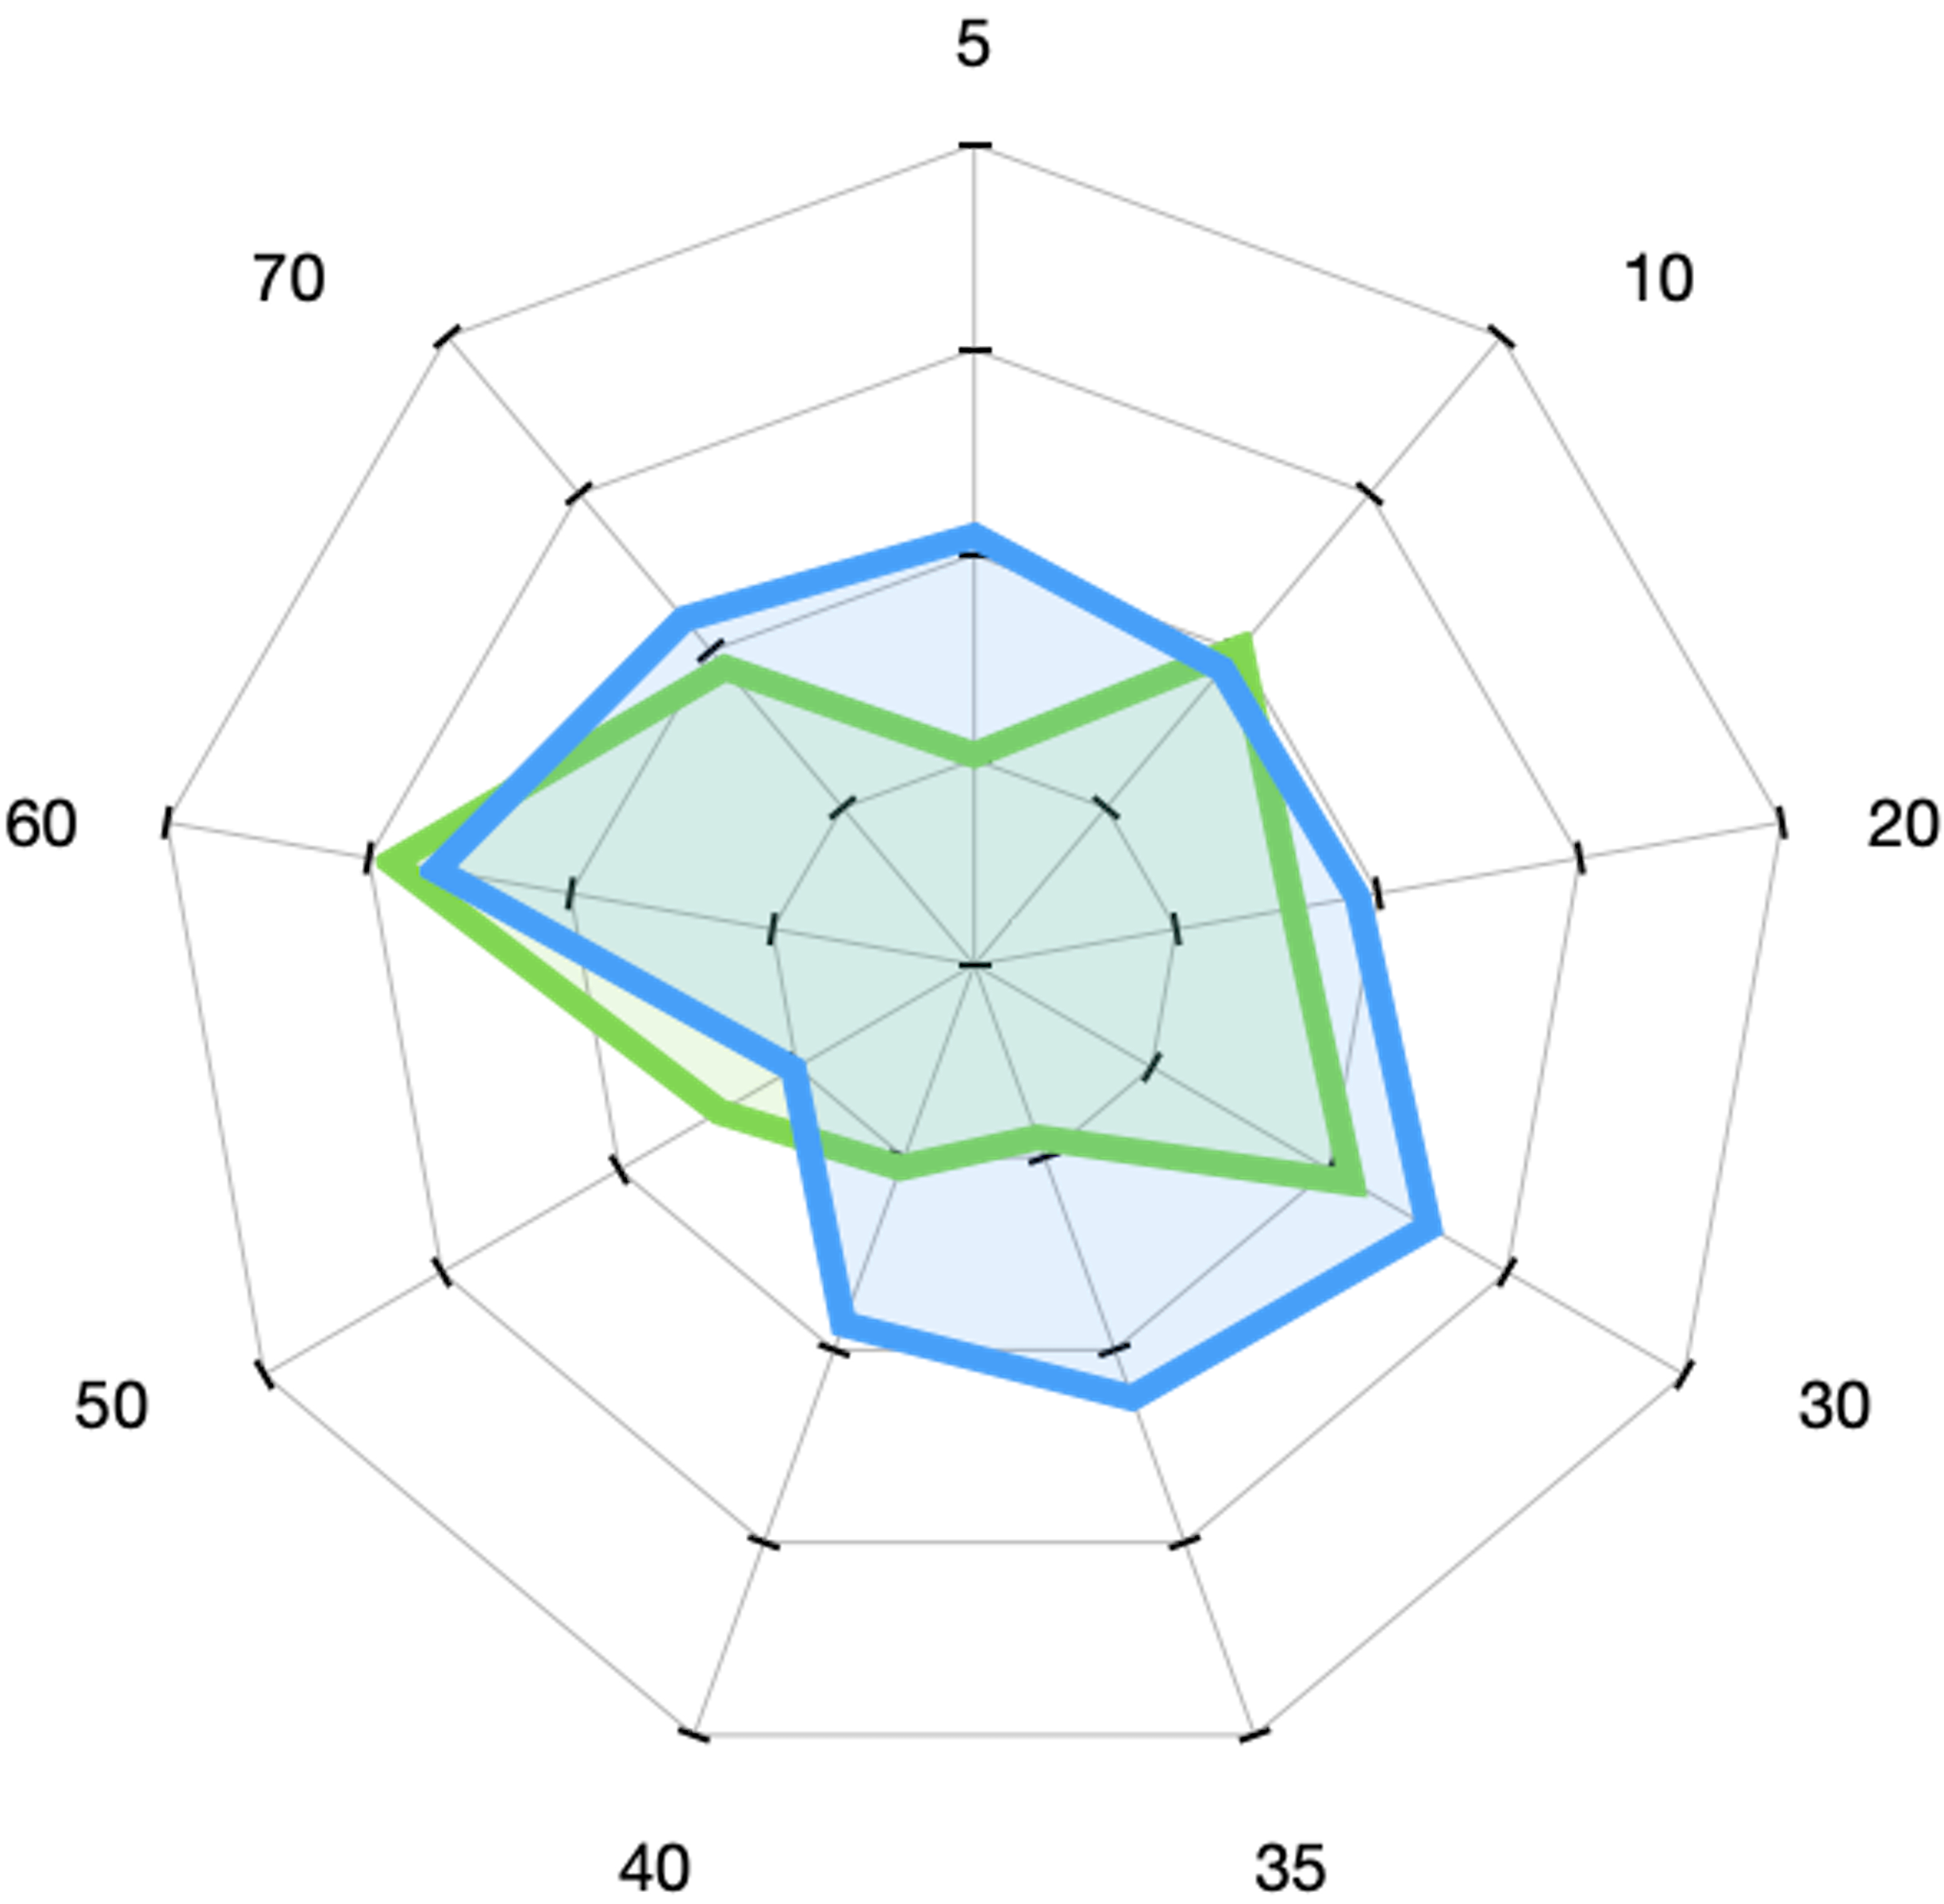
\includegraphics[width=0.4\textwidth, height=0.25\linewidth]{BI-LSTM_RMSE_SPIDER.png}\label{fig:BiLSTM_RMSE_SPIDER}}
\hfill
\subfloat[GRU: UD-Batch ensemble Vs CUD ensemble]{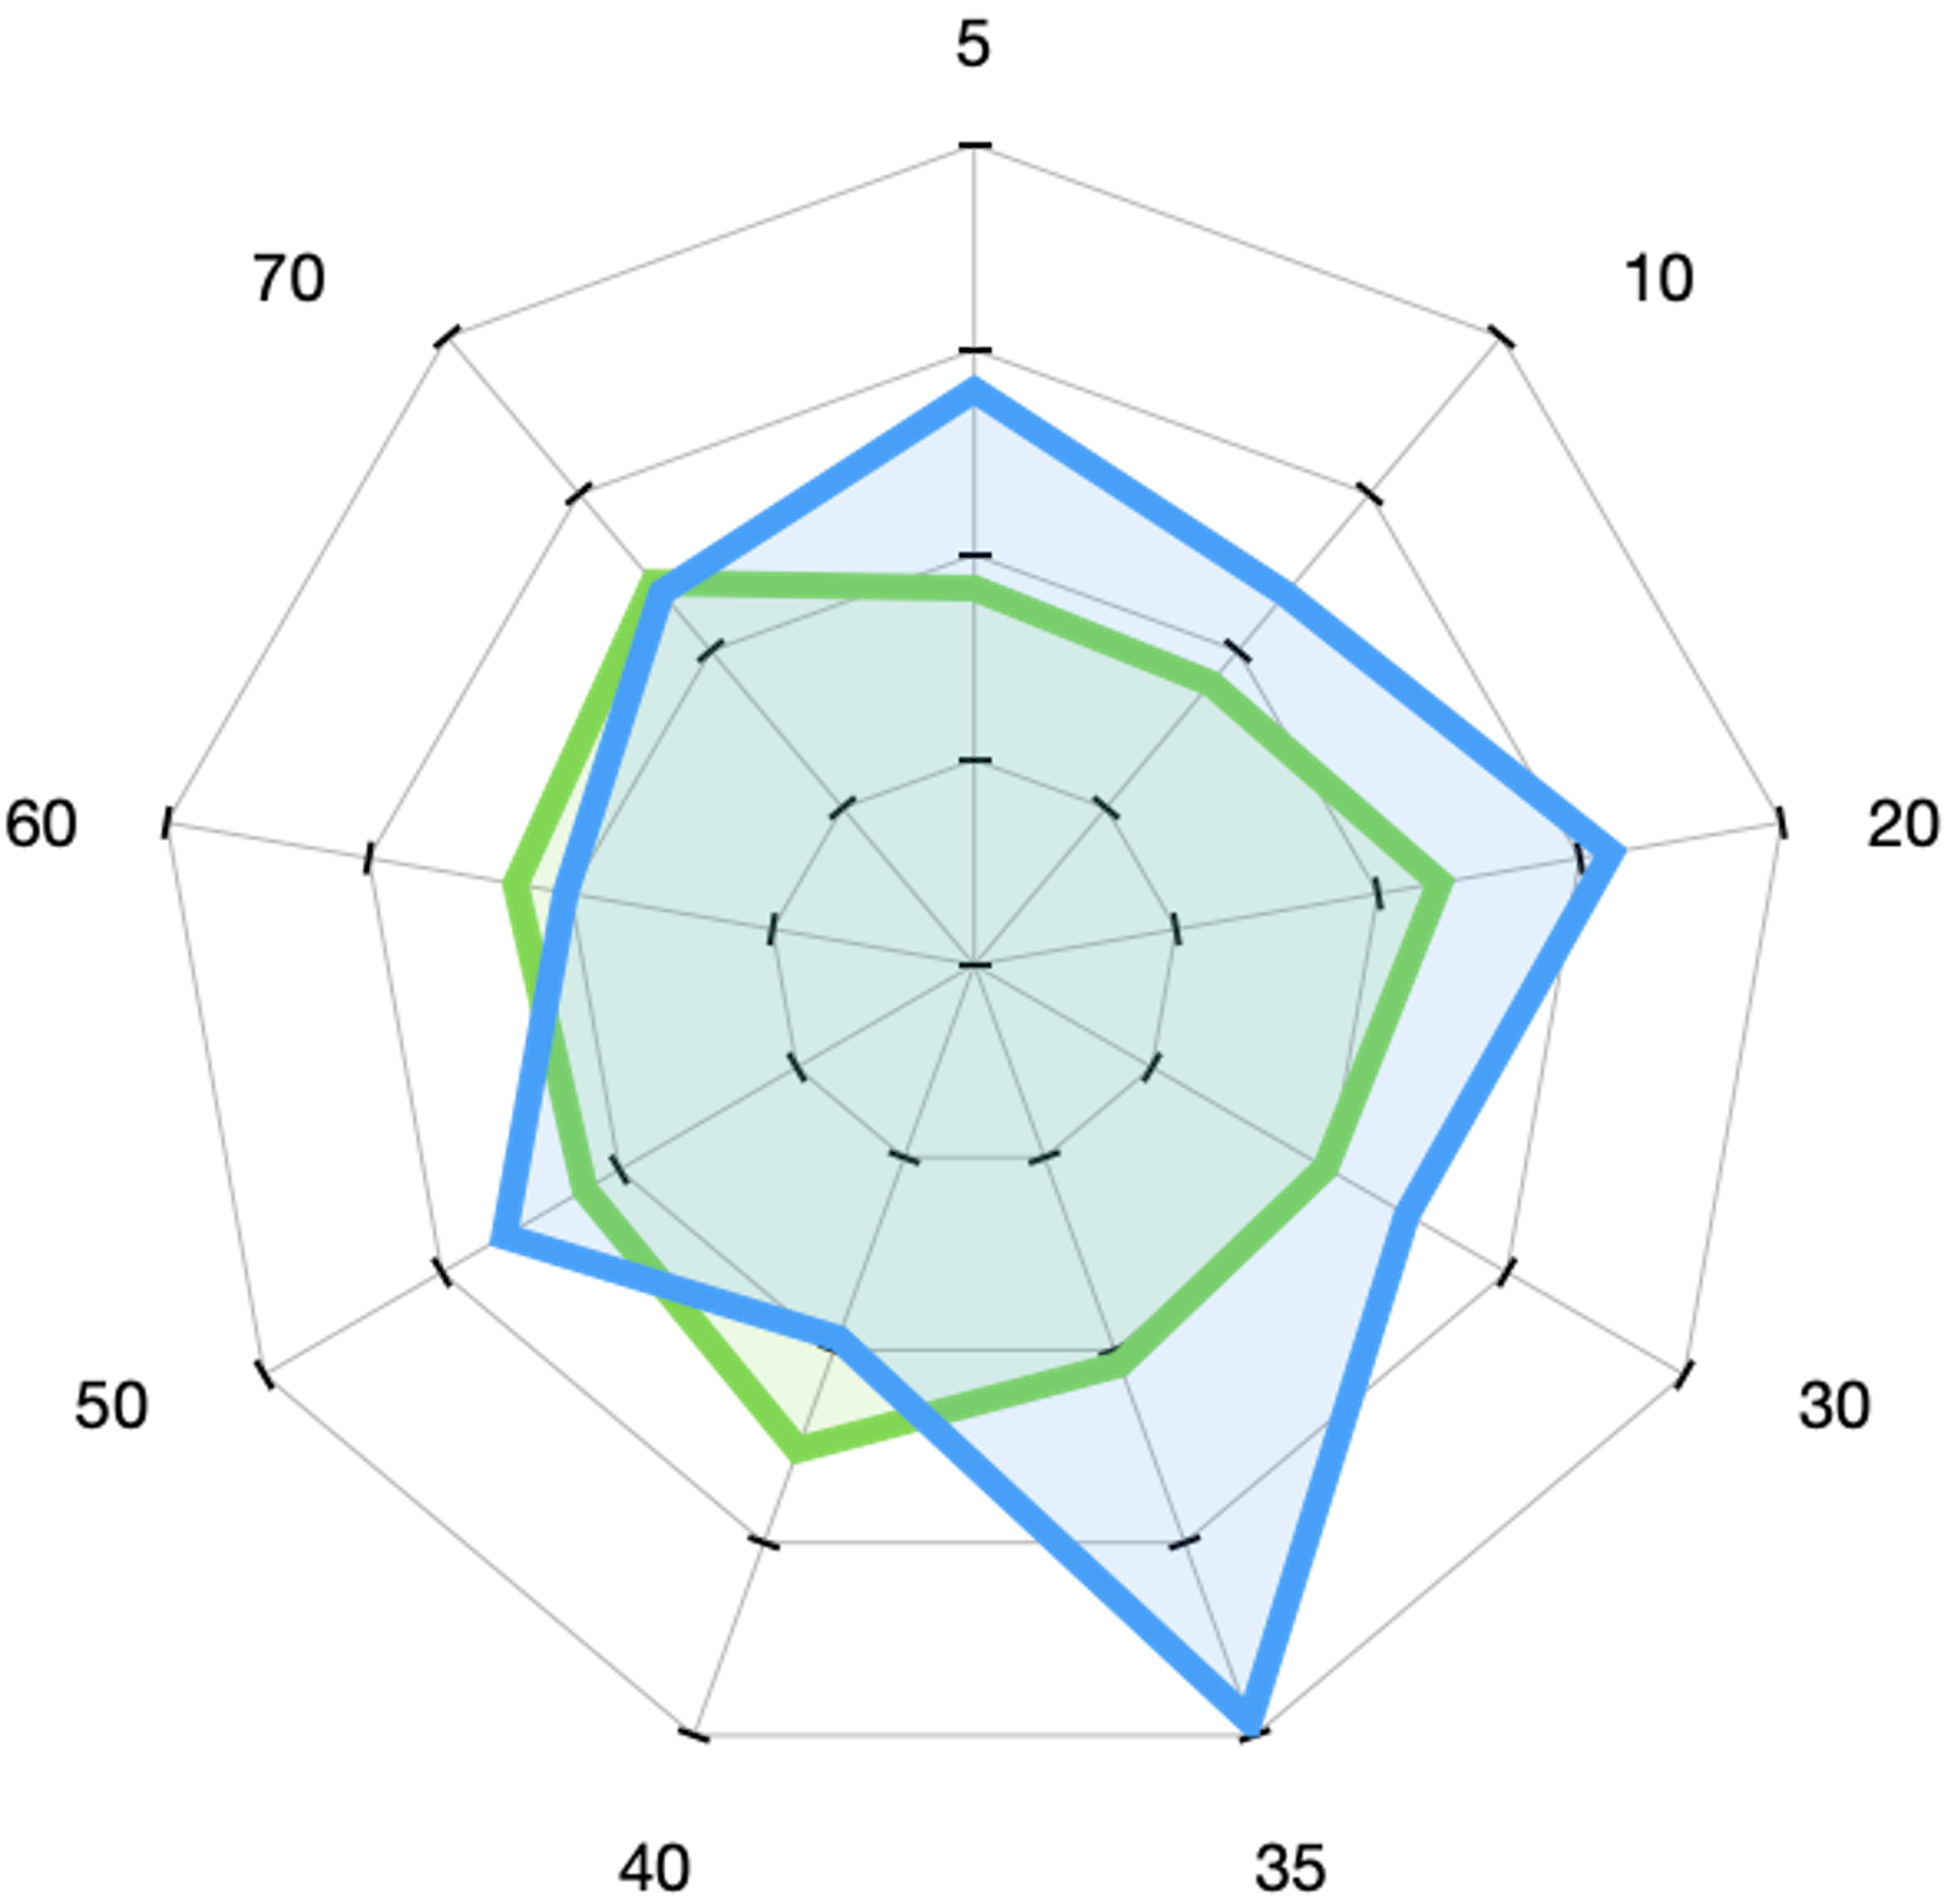
\includegraphics[width=0.4\textwidth, height=0.25\linewidth]{GRU_RMSE_SPIDER.png}\label{fig:GRU_RMSE_SPIDER}}
\caption{Performance comparison of Upward batch and Downward batch ensemble(UD-Batch) and Corresponding upward and downward ensemble(CUD-ensemble) using DL models over RMSE performance measure.}
\label{fig:all_models_rmse}
\end{figure}


\begin{figure}[ht!]
%\centering
\subfloat[LSTM: UD-Batch ensemble Vs CUD ensemble]{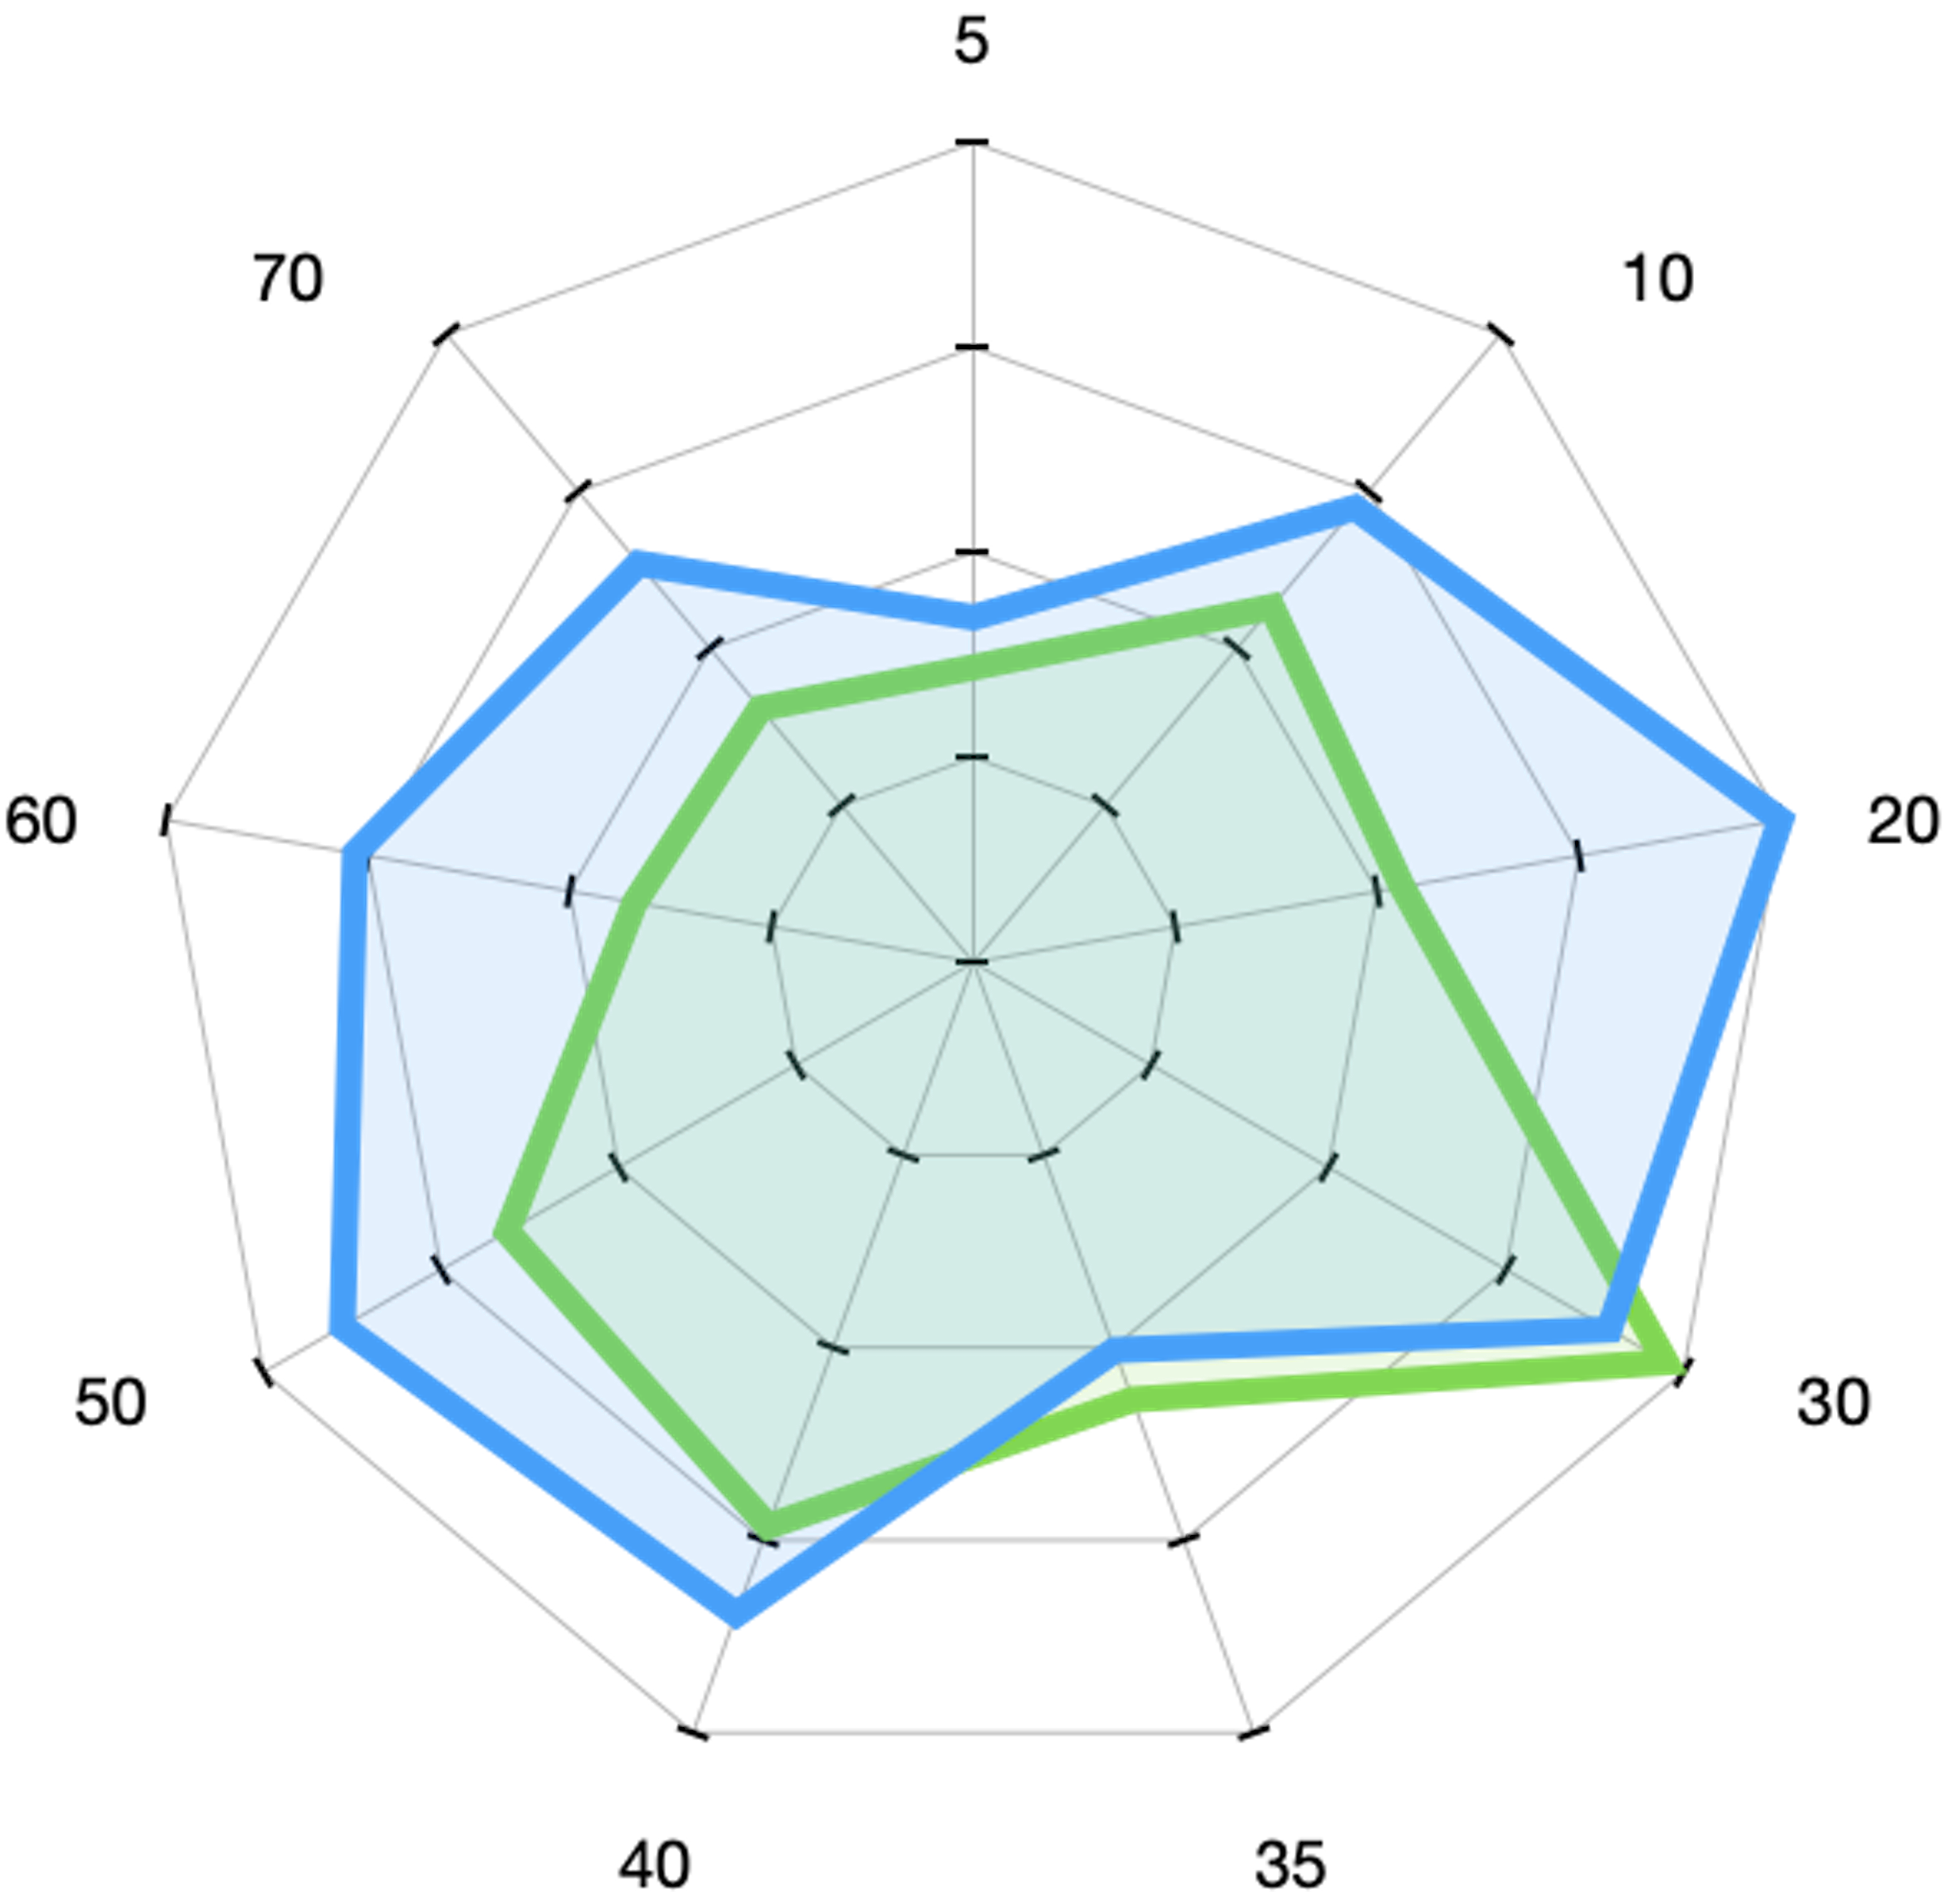
\includegraphics[width=0.4\textwidth, height=0.25\linewidth]{LSTM_RMSE_SPIDER.png}\label{fig:LSTM MAPE SPIDER}}
\hfill
\subfloat[RNN: UD-Batch ensemble Vs CUD ensemble]{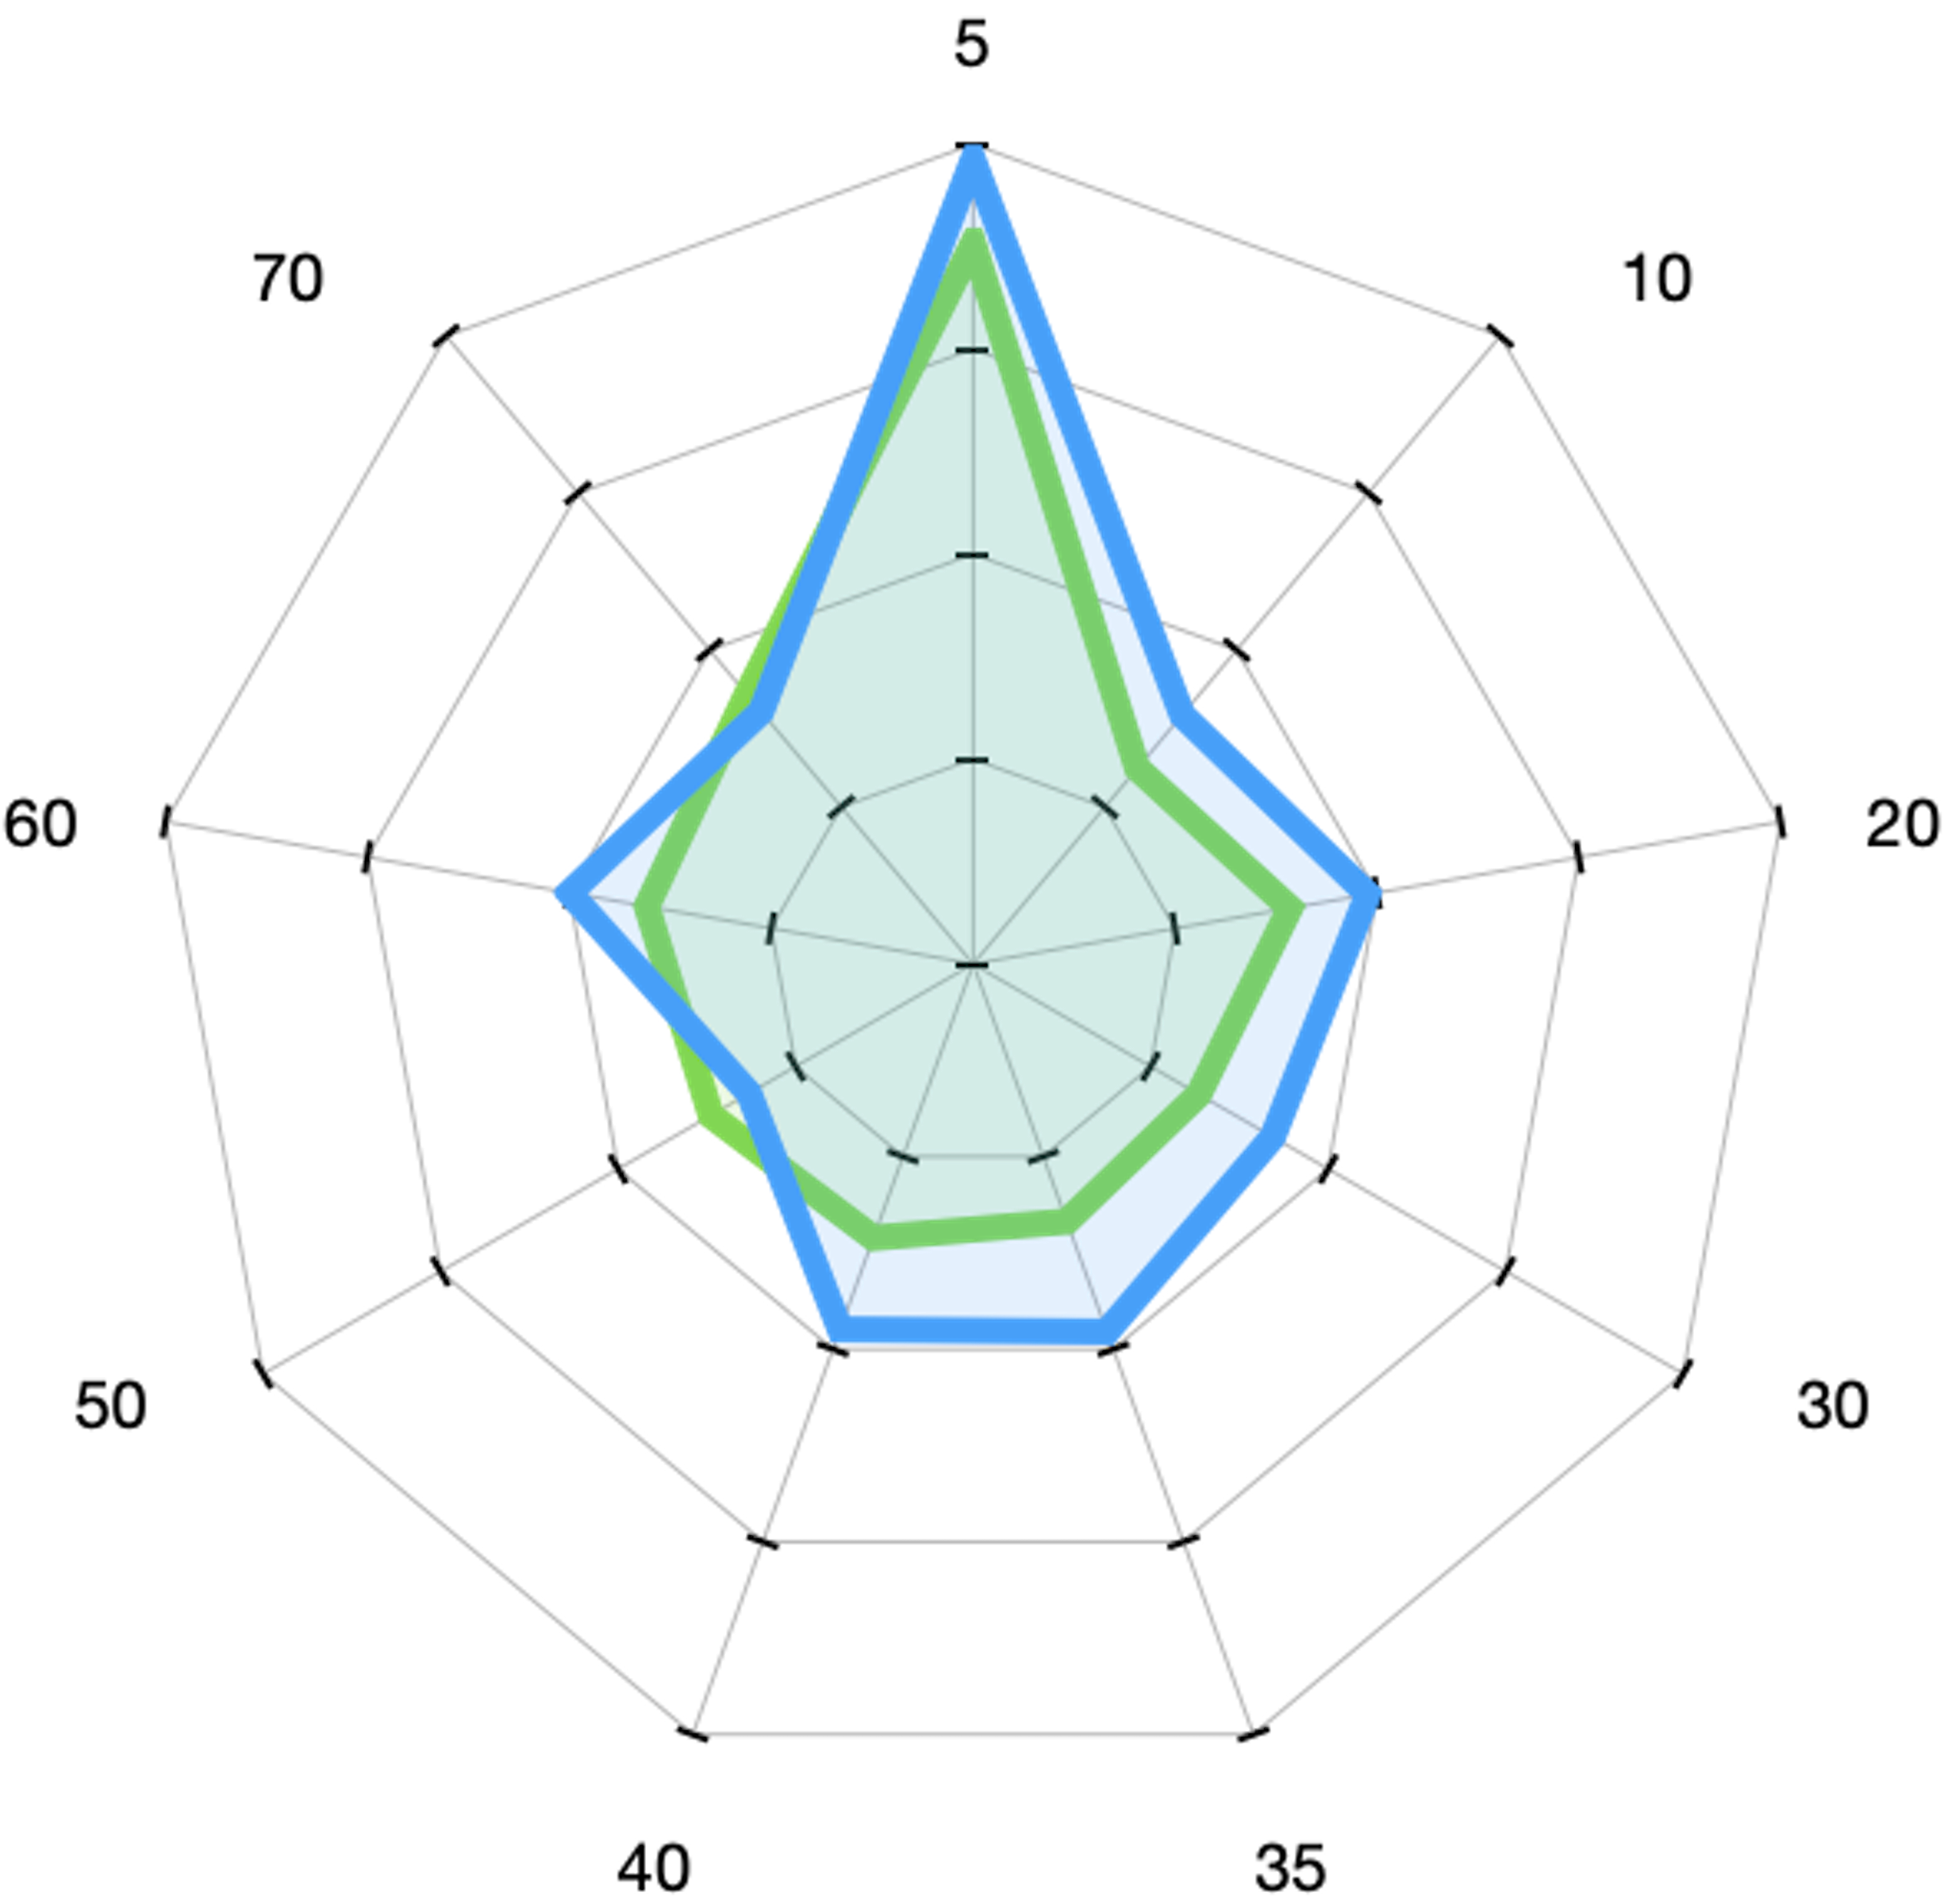
\includegraphics[width=0.4\textwidth, height=0.25\linewidth]{RNN_RMSE_SPIDER.png}\label{fig:RNN_MAPE_SPIDER}}
\\
\subfloat[BiLSTM: UD-Batch ensemble Vs CUD ensemble]{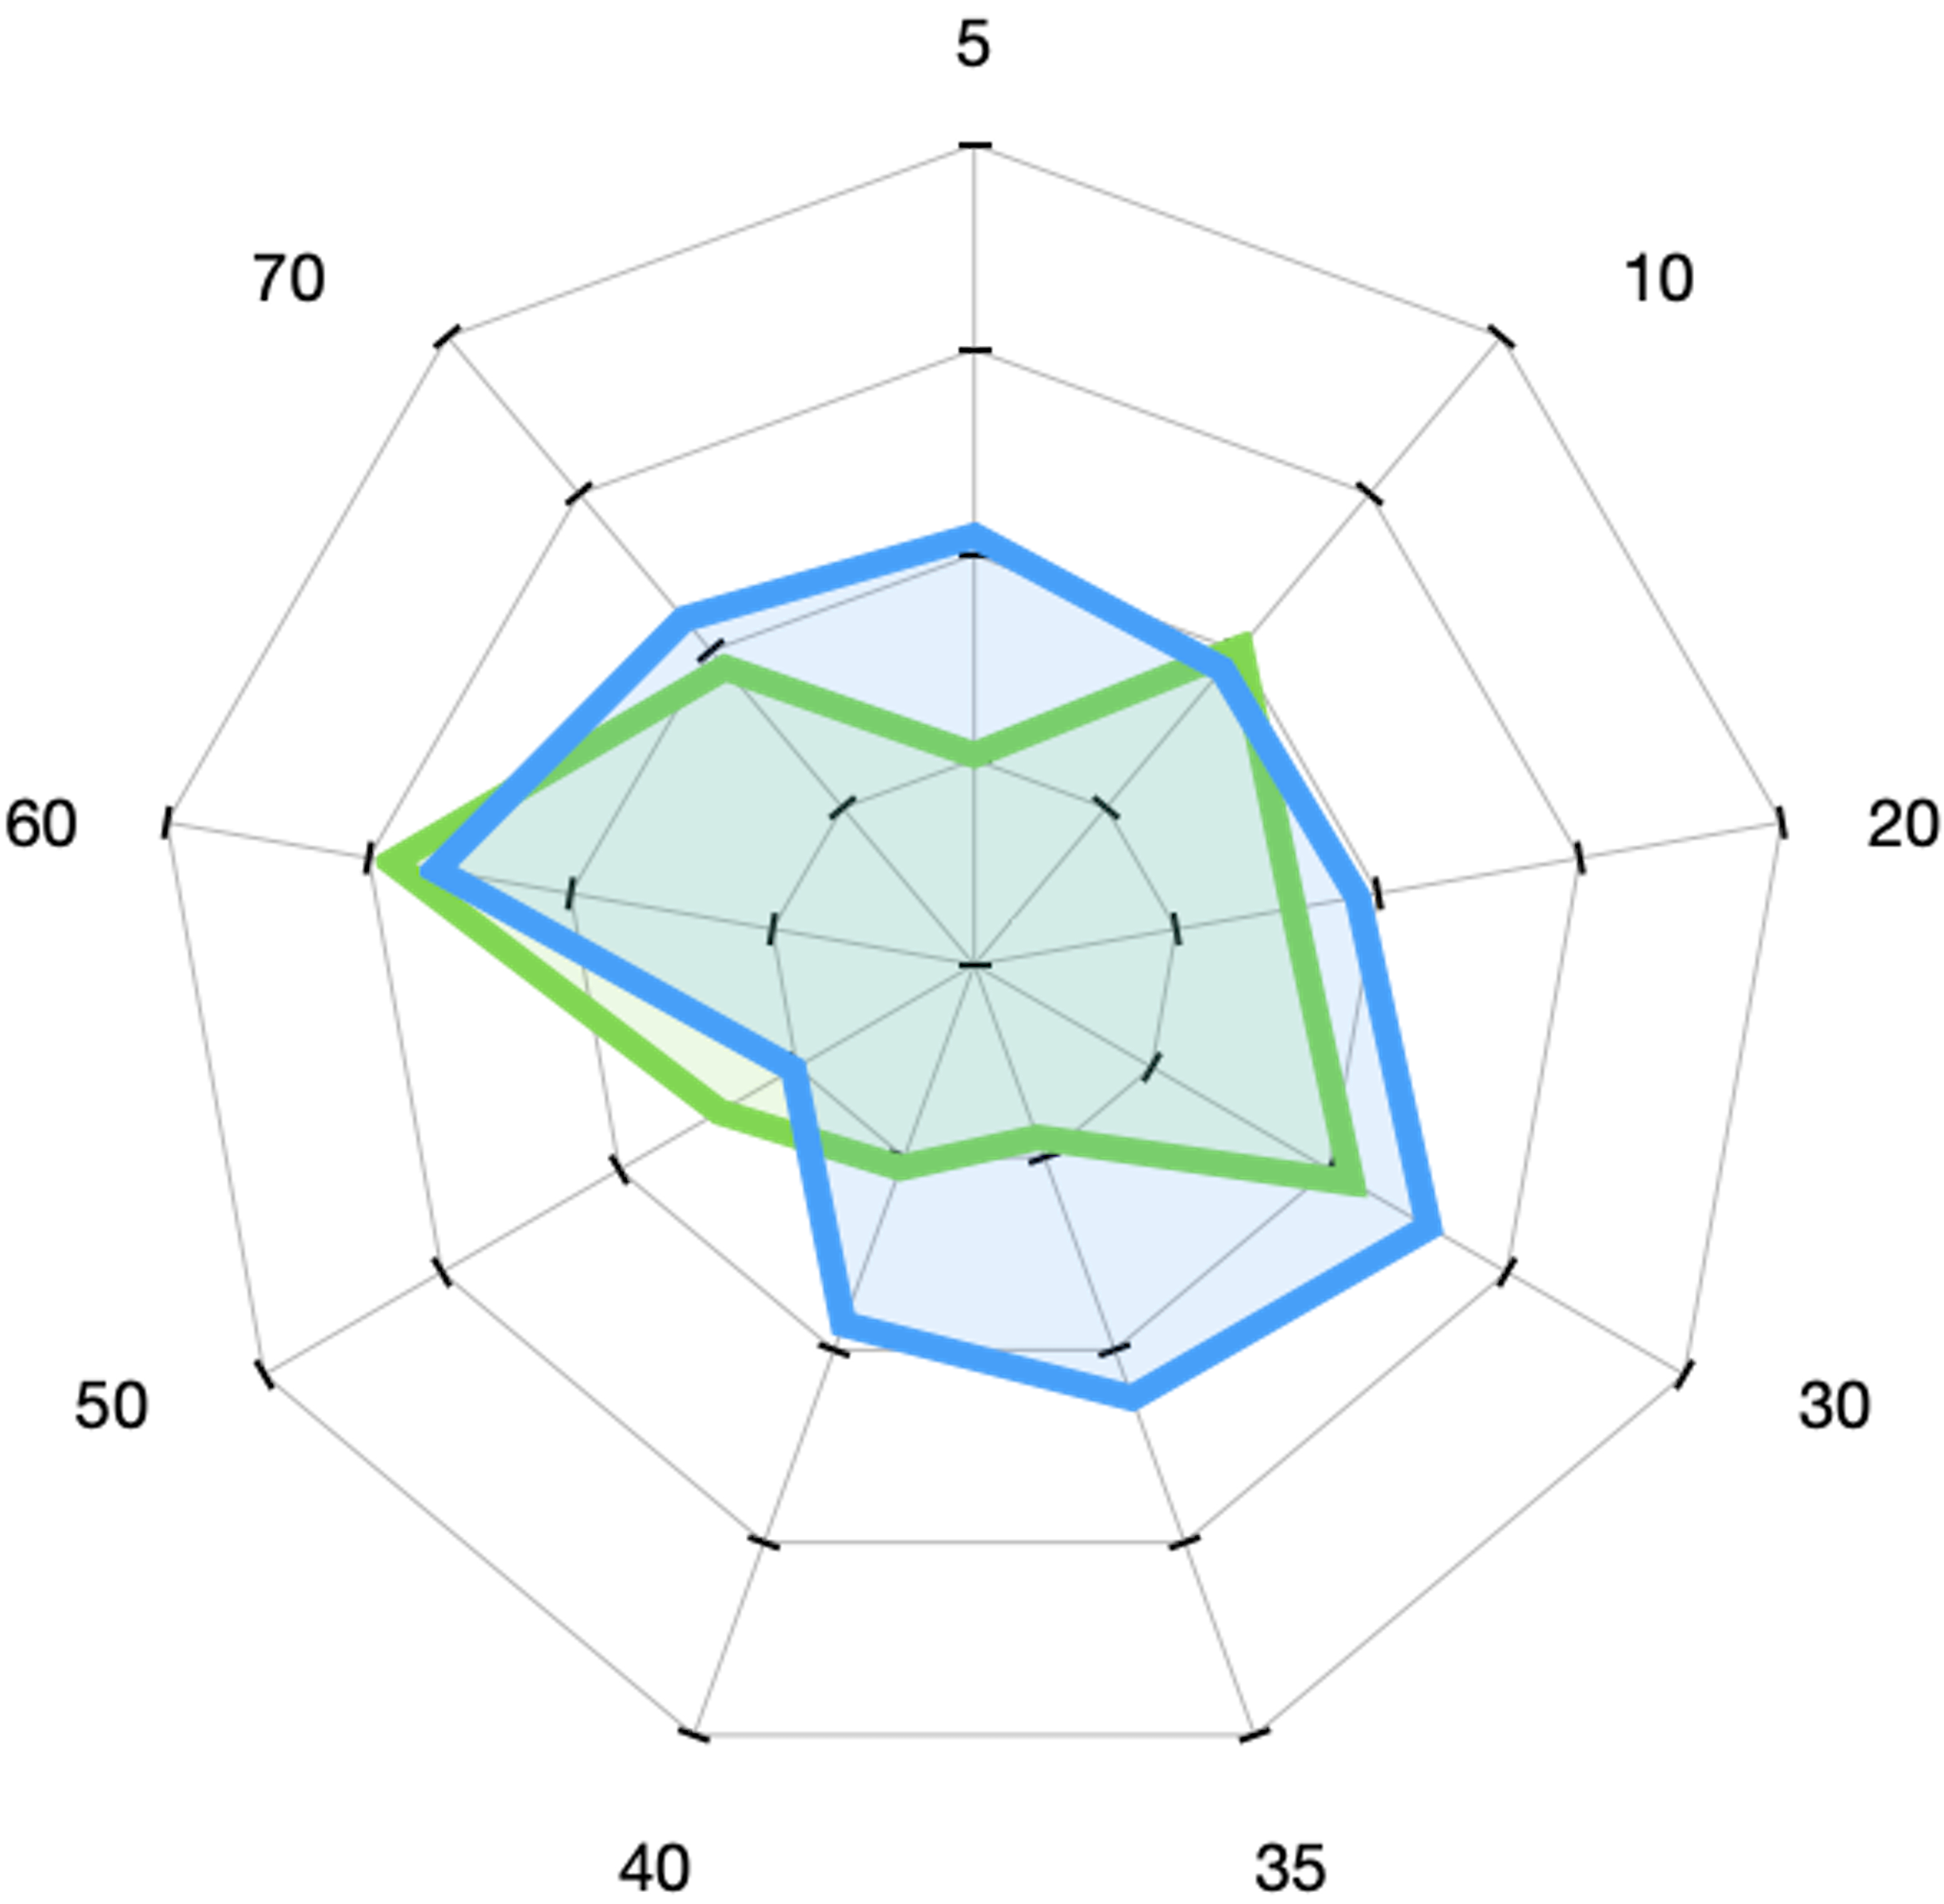
\includegraphics[width=0.4\textwidth, height=0.25\linewidth]{BI-LSTM_RMSE_SPIDER.png}\label{fig:BiLSTM_MAPE_SPIDER}}
\hfill
\subfloat[GRU: UD-Batch ensemble Vs CUD ensemble]{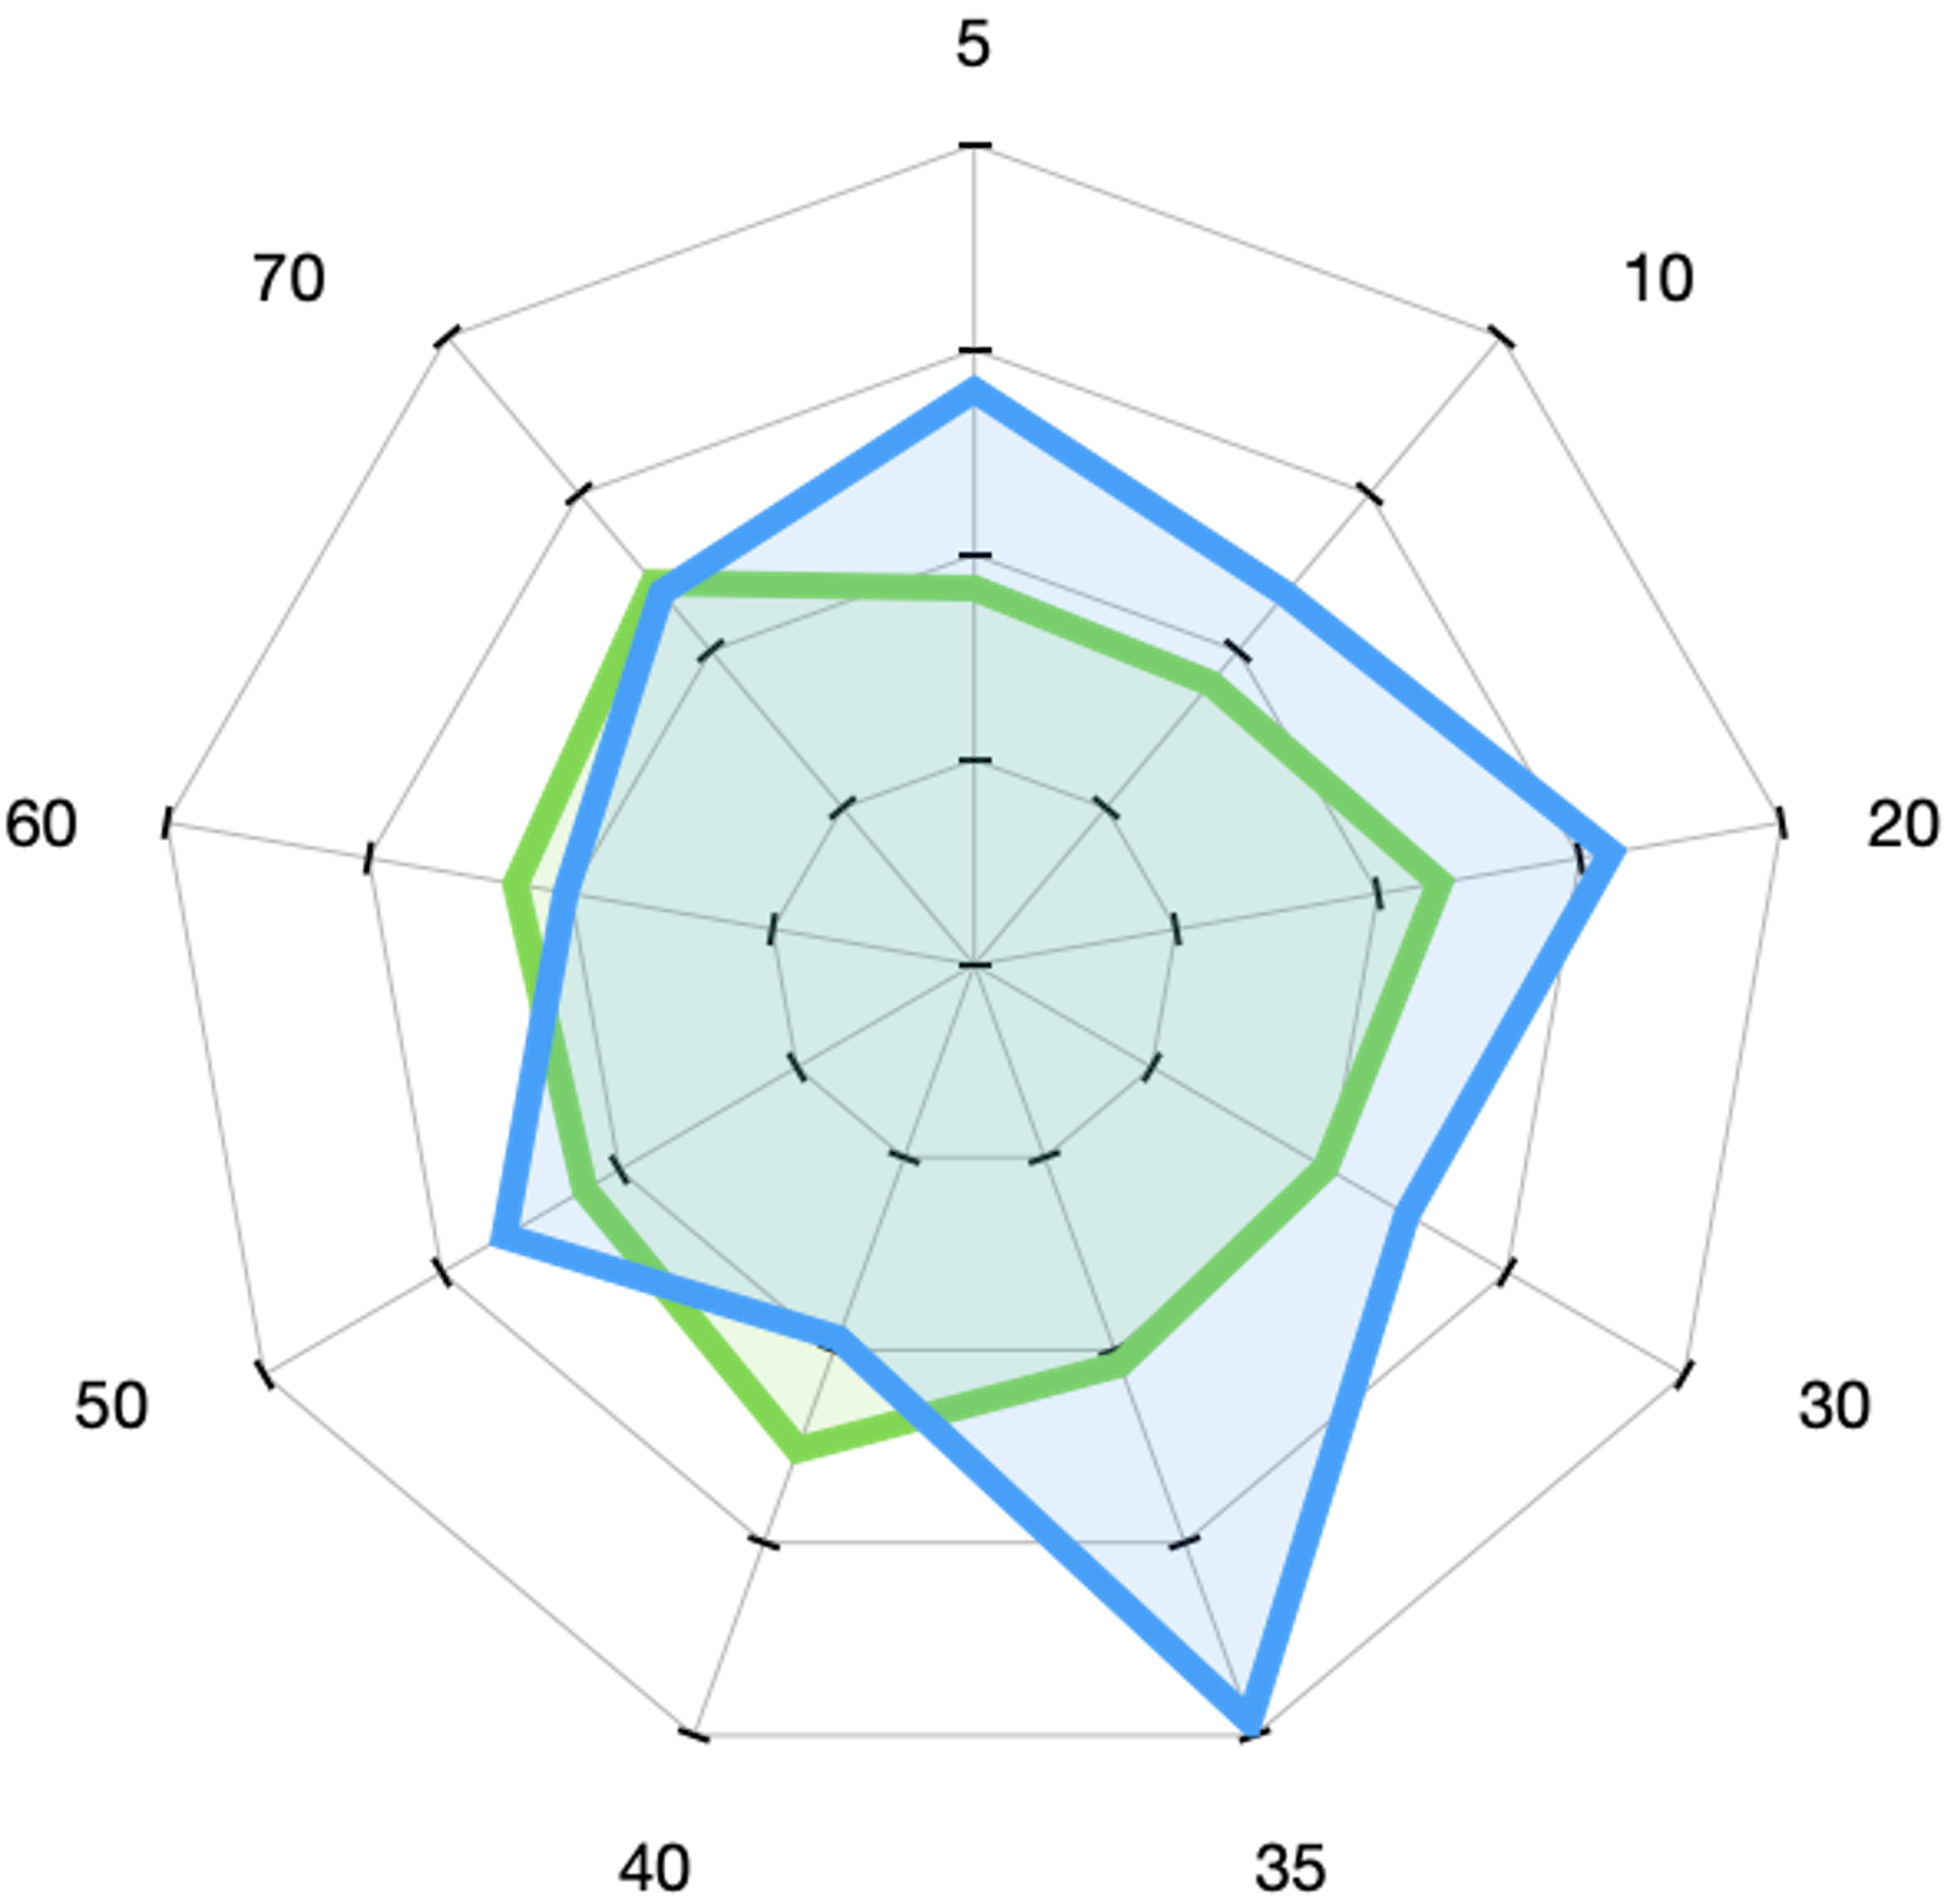
\includegraphics[width=0.4\textwidth, height=0.25\linewidth]{GRU_RMSE_SPIDER.png}\label{fig:GRU_MAPE_SPIDER}}
\caption{Performance comparison of Upward batch and Downward batch ensemble(UD-Batch) and Corresponding upward and downward ensemble(CUD-ensemble) using DL models over MAPE performance measure.}
\label{fig:all_models_mape}
\end{figure}


\begin{table}[ht!]
\centering
\caption{Performance of different DL models and proposed MBiS-DT models along \% improvement based on proposed MBiS-DT-BI-LSTM }
\label{tab:Performance_of_different DL}
\begin{tabular}{p{0.1\textwidth}lllllllll}
\hline
\textbf{MODELS} & \textbf{MSE} & \textbf{\% Imp.} & \textbf{RMSE} & \textbf{\% Imp} & \textbf{MAE} & \textbf{\% Imp} & \textbf{MAPE} & \textbf{\% Imp} \\ \hline
LSTM & 1.97 &30.96\% & 1.39 &16.54\% & 1.07 &16.82\% & 4.33 &4.61\% \\
GRU & 3.35 &59.40\% & 1.78 &34.83\% & 1.45 & 38.62\% & 4.53 &8.83\% \\
BI-LSTM & 1.62 &16.04\% & 1.26 &7.93\% & 0.99 &10.10\% & 4.41 &6.34\% \\
RNN & 1.94 &29.89\% & 1.38 &15.94\% & 1.09 &18.34\% & 4.95&16.56\% \\
\textbf{Proposed MBiS-DT-LSTM} & \textbf{1.59} &14.46\% & \textbf{1.25} &7.20\% & \textbf{0.95} &6.31\% & \textbf{4.36} &5.27\% \\
\textbf{Proposed MBiS-DT-GRU} & \textbf{1.75} &22.28\% & \textbf{1.31} &11.45\% & \textbf{1.03} & 13.59\% & \textbf{4.26} &3.05\% \\
\textbf{Proposed MBiS-DT-RNN} & \textbf{1.52} &10.52\% & \textbf{1.23} &5.69\% & \textbf{0.97} &8.24\% & \textbf{4.55} &9.23\% \\
\textbf{Proposed MBiS-DT-BI-LSTM} & \textbf{1.36} & - & \textbf{1.16} &- & \textbf{0.89} & - & \textbf{4.13} & - \\
\hline
\end{tabular}
\end{table}


Table\ref{tab:Performance_of_different DL} provides a comparative analysis of experimented  traditional models, namely LSTM, GRU, BiLSTM and RNN and proposed models namely Proposed MBiS-DT-LSTM,   Proposed MBiS-DT-GRU,  Proposed MBiS-DT-RNN,  Proposed MBiS-DT-BI-LSTM based on key performance metrics, including MSE,  RMSE,  MAE  and MAPE.  The model Proposed MBiS-DT-BI-LSTM is best performar over other traditional models and proposed models so in terms of RMSE the maximum improvement is 34.83\%  then GRU and minimum improvement is 5.69\% then Proposed MBiS-DT-RNN.  In terms of MSE the maximum improvement is 59.40\%  then GRU and minimum improvement is 10.52\% then Proposed MBiS-DT-RNN.  In terms of MAE the maximum improvement is 38.62\%  then GRU and minimum improvement is 8.24\% then Proposed MBiS-DT-RNN.  In terms of MAPE the maximum improvement is 16.56\%  then RNN and minimum improvement is 3.05\% then Proposed MBiS-DT-GRU.


% \begin{table}[ht!]
% \centering
% \caption{MAPE}
% \label{tab:MAPE}
% \begin{tabular}{lllll}
% \hline
% \textbf{MODELS} & \textbf{ORIGINAL} & \textbf{\% IMPROVEMENT} & \textbf{PROPOSED (P)} & \textbf{SHIFT LENGTH} \\ \hline
% \textbf{LSTM} & 4.33 & -7.78 & 4.36 & 20 \\
% \textbf{GRU} & 4.53 & 6.10 & 4.26 & 35 \\
% \textbf{BI-LSTM} & 4.41 & 6.31 & 4.13 & 35 \\
% \textbf{RNN} & 4.95 & 8.10 & 4.55 & 35 \\ \hline
% \end{tabular}
% \end{table}

% \begin{table}[ht!]
% \centering
% \caption{RMSE}
% \label{tab:RMSE}
% \begin{tabular}{lllll}
% \hline
% \textbf{MODELS} & \textbf{ORIGINAL} & \textbf{\% IMPROVEMENT} & \textbf{PROPOSED (P)} & \textbf{SHIFT LENGTH} \\ \hline
% \textbf{LSTM} & 1.39 & 10.0381 & 1.2593 & 20 \\
% \textbf{GRU} & 1.78 & 25.98 & 1.31 & 35 \\
% \textbf{BI-LSTM} & 1.26 & 7.99 & 1.16 & 35 \\
% \textbf{RNN} & 1.38 & 10.38 & 1.2343 & 35 \\ \hline
% \end{tabular}
% \end{table}
% \begin{table}[ht!]
% \centering
% \caption{MAE}
% \label{tab:MAE}
% \begin{tabular}{lllll}
% \hline
% \textbf{MODELS} & \textbf{ORIGINAL} & \textbf{\% IMPROVEMENT} & \textbf{PROPOSED (P)} & \textbf{SHIFT LENGTH} \\ \hline
% \textbf{LSTM} & 1.07 & 11.20 & 0.95 & 20 \\
% \textbf{GRU} & 1.45 & 28.8 & 1.03 & 35 \\
% \textbf{BI-LSTM} & 0.99 & 10.10 & 0.89 & 35 \\
% \textbf{RNN} & 1.09 & 11.24 & 0.97 & 35 \\ \hline
% \end{tabular}
% \end{table}


%\centering


\begin{figure}
    \centering
    \includegraphics[scale=0.23]{line_Plot.png}
    \caption{Prediction plot of original test data(subset) and corresponding to traditional DL models and proposed MBiS-DT + DL's models.}
    \label{fig:Line plot of vs proposed MBiS-DT models}
\end{figure}

In this line plot of tradition models and proposed model prediction along with test data shows that our proposed models are close to test data then tradition models fig.\ref{fig:Line plot of vs proposed MBiS-DT models} .  For clear visualization we have used sub part (40 data points.) of test data.   Overall, the line plot's results support the conclusion that the proposed models are indeed better choices for temperature prediction than the traditional models, making them valuable tools for meteorological forecasting and related applications.

\begin{figure}
    \centering
    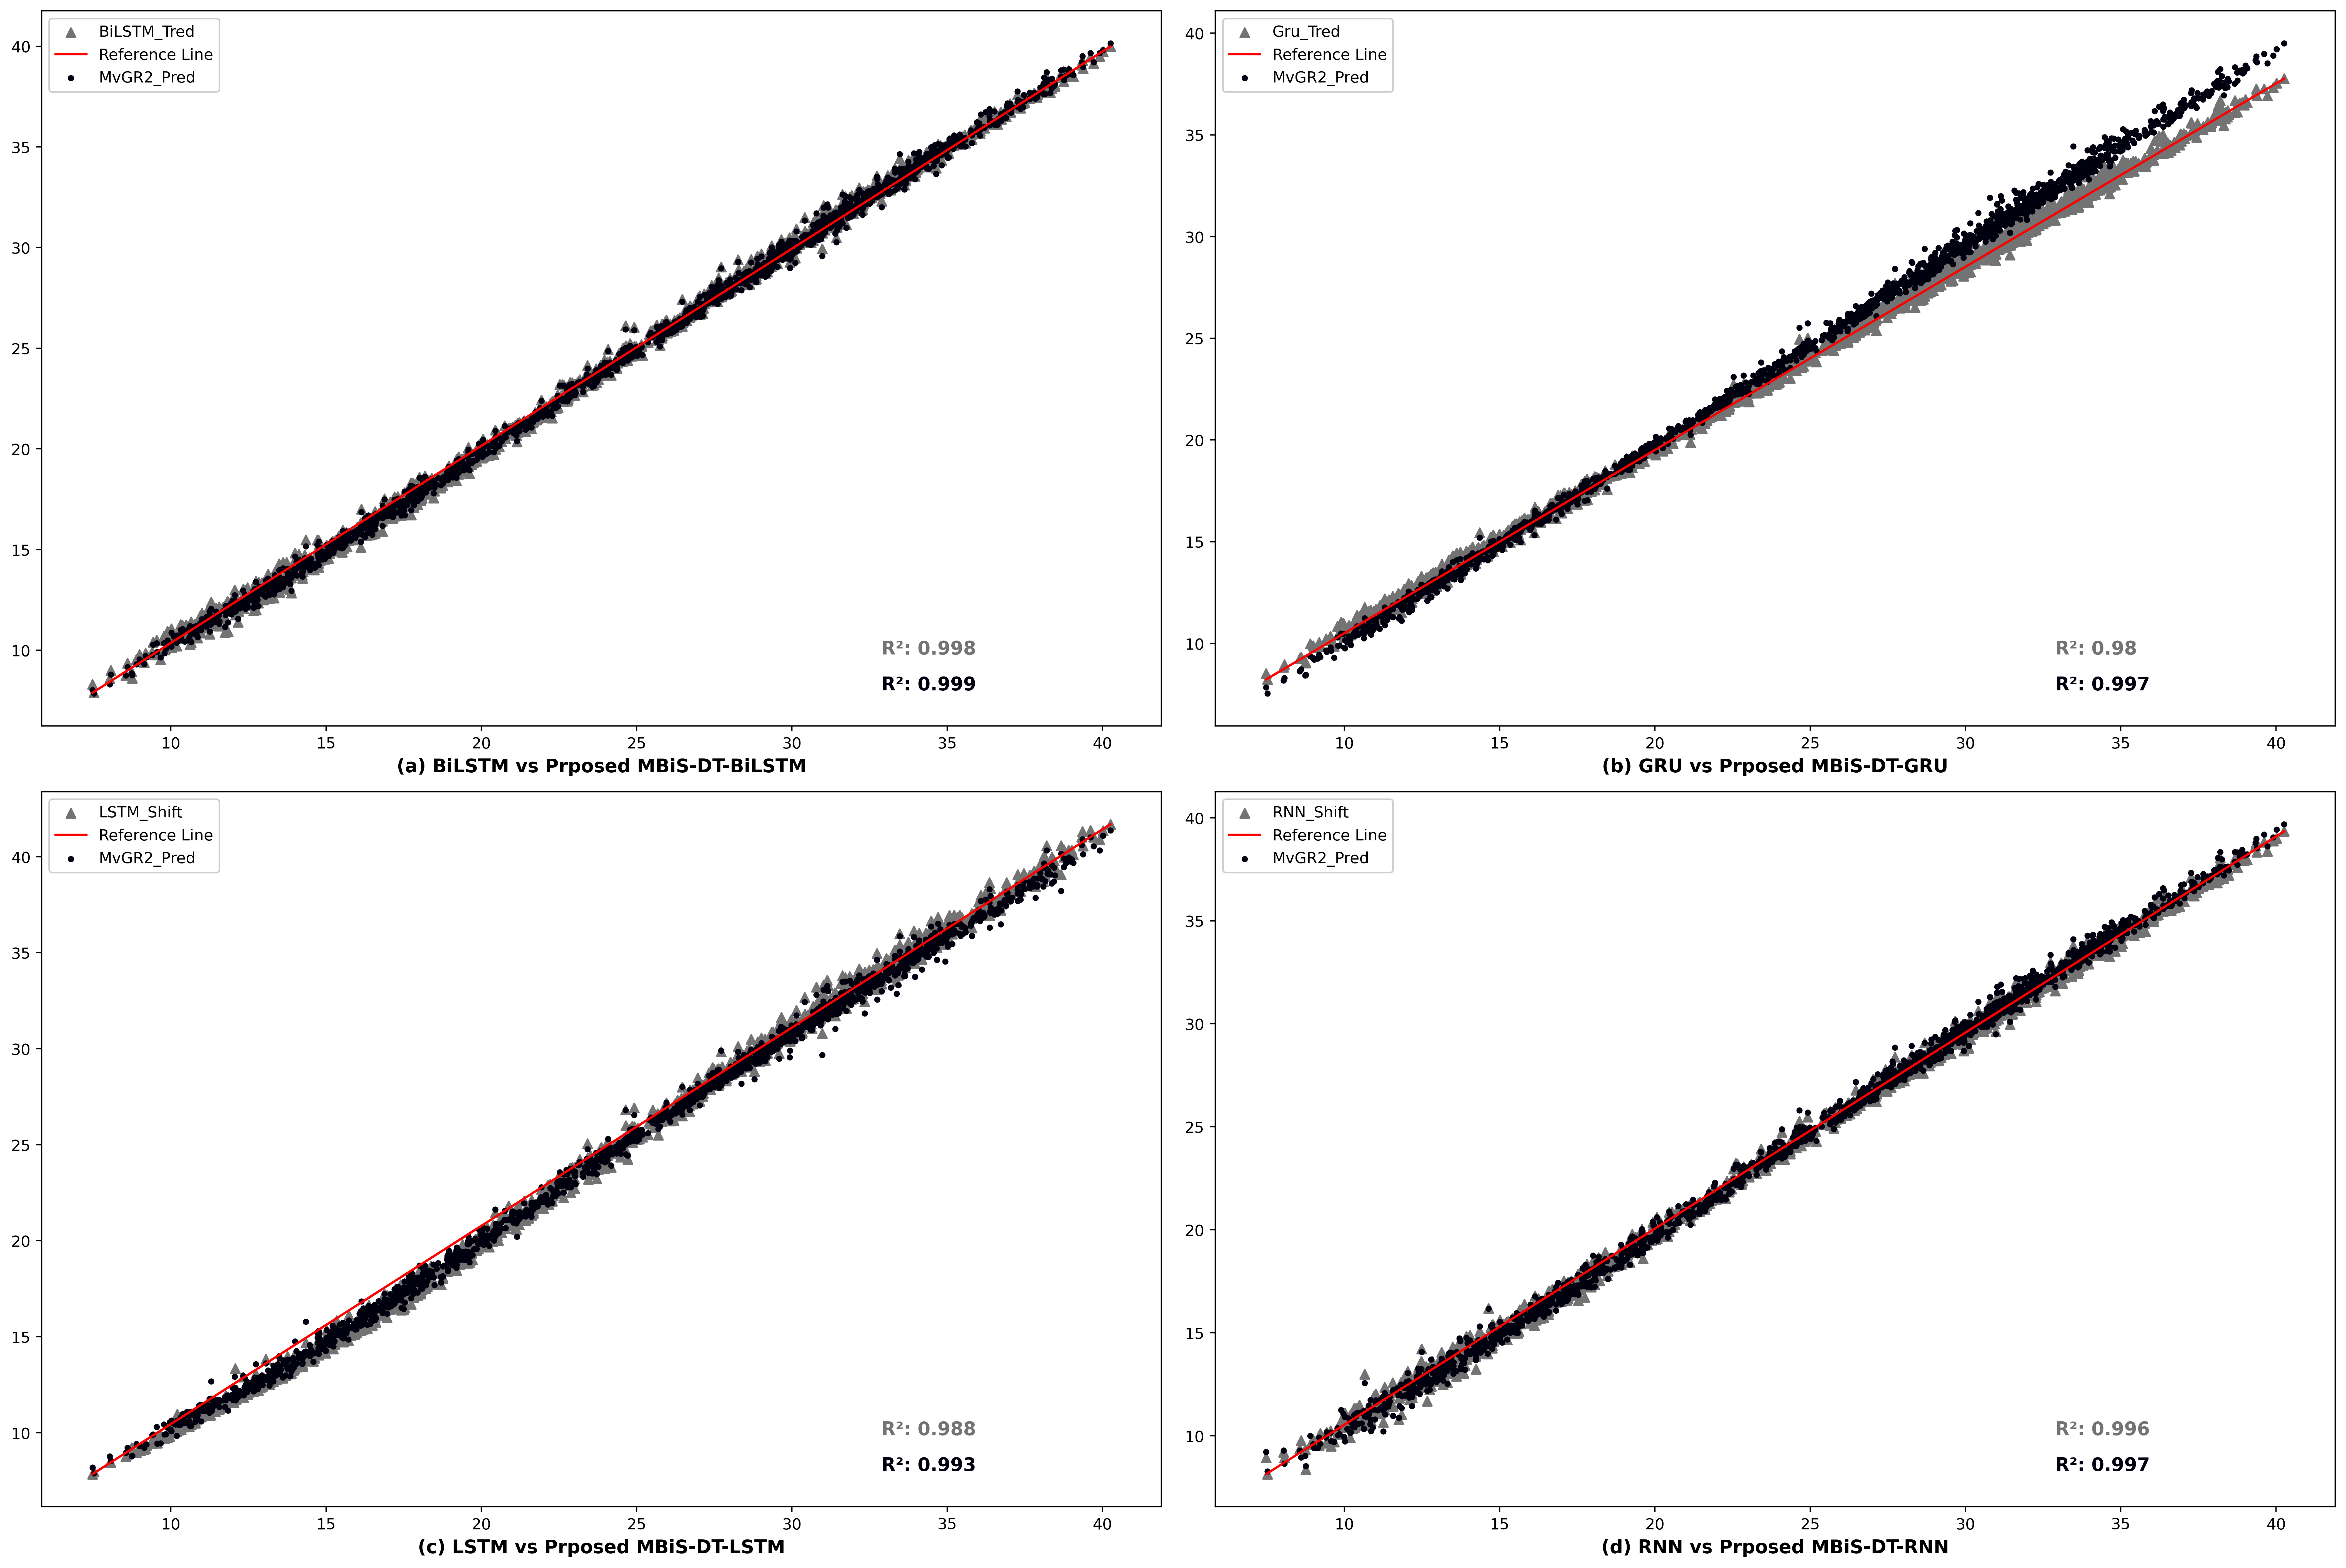
\includegraphics[scale=0.25]{scatter_Plot.png}
    \caption{Superimposed Prediction Scattered plot of traditional DL and proposed model over test data.}
    \label{fig:Scatter plot of vs proposed MBiS-DT models}
\end{figure}



In fig.\ref{fig:Scatter plot of vs proposed MBiS-DT model}, the superimposed prediction scattered plot of traditional DL and proposed model over test data shows that the distribution of points are closest to trend line.   The R\^2 values for RNN,  GRU,  BiLSTM,  LSTM are 0.996,  0.98,  0.998,  0.988 respectively and values for Proposed MBiS-DT-RNN,  Proposed MBiS-DT-GRU,  Proposed MBiS-DT-LSTM  Proposed MBiS-DT-BI-LSTM  are 0.997,  0.997,  0.993,  0.999.  The grater value of R\^2 shows the preciseness of data so our proposed models have grater R\^2 values then traditional models .  The conclusion of of this plot is our proposed models are performing better then traditional models.
%\section{This is an example for first level head---section head}\label{sec3}
\begin{figure}[ht!]
\centering
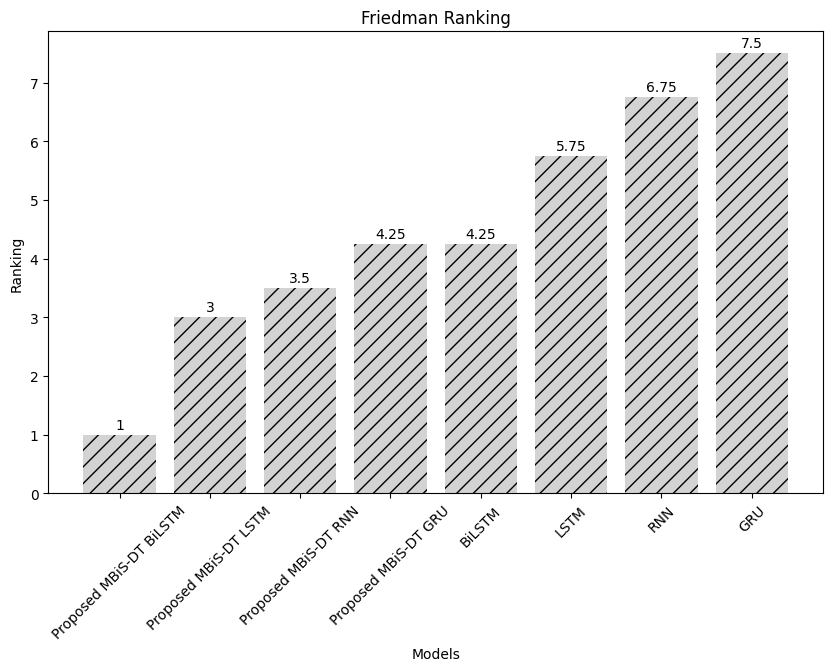
\includegraphics[width=0.9\textwidth, height=0.6\linewidth]{freidman_rank.png}
\label{fig:Friedman}
\caption{Aggregated Friedman Ranking of proposed (MBiS-DT) models and traditional models over RMSE, MAE, MSE and MAPE.}
\end{figure}

\begin{table}[ht!]
\begin{tabular}{l|lllll}
\hline
\\
Models& MSE & RMSE & MAE & MAPE & Friedman Ranking\\
\hline
\\
LSTM & 7 & 7 & 6 & 3 & 5.75 \\
GRU & 8 & 8 & 8 & 6 &7.5 \\
BiLSTM & 4 & 4 & 4 & 5 &4.25 \\
RNN & 6 & 6 & 7 & 8 &6.75 \\
Proposed LSTM & 3 & 3 & 2 & 4 & 3 \\
Proposed GRU & 5 & 5 & 5 & 2 &4.25 \\
Proposed BiLSTM & 1 & 1 & 1 & 1 &1 \\
Proposed RNN & 2 & 2 & 3 & 7 &3.5 \\ \hline
\end{tabular}
\caption{Ranking of Different Models based on performance measures}
\label{tab:Friedman}
\end{table}
The Parametric Friedman Ranking of all experimented models is represented in Table \ref{tab:Friedman}

%\begin{table}[!htp]
%\centering
%\begin{tabular}{|c|c|}\hline
%Algorithm&Ranking\\\hline
%LSTM & 5.75\\
%GRU & 7.5\\
%BiLSTM & 4.25\\
%RNN & 6.75\\
%Proposed LSTM & 3\\
%Proposed GRU & 4.25\\
%Proposed BiLSTM & 1\\
%Proposed RNN & 3.5\\
%\hline
%\end{tabular}
%\caption{Average Rankings of the algorithms}
%\label{tab:Friedman}
%\end{table}
Adjusted p-values for $\alpha$=0.05 is represented in Table \ref{tab:pvalue}
%\begin{table}[!htp]
%\centering\scriptsize
%\begin{tabular}{cccc}
%$i$&algorithms&$z=(R_0 - R_i)/SE$&$p$\\
%\hline6&GRU vs. BiLSTM&2.738613&\textbf{0.00617\\
%5&LSTM vs. BiLSTM&1.917029&0.055234\\
%4&BiLSTM vs. RNN&1.917029&0.055234\\
%3&LSTM vs. GRU&0.821584&0.411314\\
%2&GRU vs. RNN&0.821584&0.411314\\
%1&LSTM vs. RNN&0&1\\
%\hline
%\end{tabular}
%\caption{P-values Table for $\alpha=0.05$}
%\label{tab:pvalue}
%\end{table}

\begin{table}[!htbp]
\centering\scriptsize
\begin{tabular}{cccc}
\hline
$i$&algorithms&$z=(R_0 - R_i)/SE$&$p$\\
\hline28&GRU vs. Proposed BiLSTM&3.752777&\textbf{0.000175}\\
27&RNN vs. Proposed BiLSTM&3.319764&\textbf{0.000901}\\
26&LSTM vs. Proposed BiLSTM&2.742414&\textbf{0.006099}\\
25&GRU vs. Proposed LSTM&2.598076&\textbf{0.009375}\\
24&GRU vs. Proposed RNN&2.309401&\textbf{0.020921}\\
23&RNN vs. Proposed LSTM&2.165064&\textbf{0.030383}\\
22&GRU vs. BiLSTM&1.876388&0.060602\\
21&GRU vs. Proposed GRU&1.876388&0.060602\\
20&BiLSTM vs. Proposed BiLSTM&1.876388&0.060602\\
19&RNN vs. Proposed RNN&1.876388&0.060602\\
18&Proposed GRU vs. Proposed BiLSTM&1.876388&0.060602\\
17&LSTM vs. Proposed LSTM&1.587713&0.112351\\
16&BiLSTM vs. RNN&1.443376&0.148915\\
15&RNN vs. Proposed GRU&1.443376&0.148915\\
14&Proposed BiLSTM vs. Proposed RNN&1.443376&0.148915\\
13&LSTM vs. Proposed RNN&1.299038&0.193931\\
12&Proposed LSTM vs. Proposed BiLSTM&1.154701&0.248213\\
11&LSTM vs. GRU&1.010363&0.312321\\
10&LSTM vs. BiLSTM&0.866025&0.386476\\
9&LSTM vs. Proposed GRU&0.866025&0.386476\\
8&BiLSTM vs. Proposed LSTM&0.721688&0.470486\\
7&Proposed LSTM vs. Proposed GRU&0.721688&0.470486\\
6&LSTM vs. RNN&0.57735&0.563703\\
5&GRU vs. RNN&0.433013&0.665006\\
4&BiLSTM vs. Proposed RNN&0.433013&0.665006\\
3&Proposed GRU vs. Proposed RNN&0.433013&0.665006\\
2&Proposed LSTM vs. Proposed RNN&0.288675&0.77283\\
1&BiLSTM vs. Proposed GRU&0&1\\
\hline
\end{tabular}
\caption{P-values Table for $\alpha=0.05$}
\label{tab:pvalue}
\end{table}
\pagebreak

\section{Conclusion}
In this study, a DL approach has been utilized to forecast the temperature. In this research endeavour, the potential of DL in enhancing temperature prediction has been explored. The intricate interplay between temperature and DL techniques has been illuminated, offering insights into the accuracy and efficacy of data-driven prediction models.

Through an in-depth investigation into time-series satellite data and using DL methodologies, our study has underscored the capacity of neural networks to capture complex temporal dependencies within temperature patterns. This capacity extends to short and mid-term predictions, where the predictive performance showcases the power of data-driven insights.

Our research journey encompassed the intricate modelling of temperature fluctuations, Exploring the details of how things change over time in an easy-to-understand way. By supporting the strengths of DL architectures, we have pushed the boundaries of predictive accuracy, contributing to a broader understanding of climate variations and their implications.

%\section*{Declarations}

%Some journals require declarations to be submitted in a standardized format. Please check the Instructions for Authors of the journal you are submitting to see if you need to complete this section. If yes, your manuscript must contain the following sections under the heading `Declarations':

%\begin{itemize}
%\item Funding
%\item Conflict of interest/Competing interests (check journal-specific guidelines for which heading to use)
%\item Ethics approval
%\item Consent to participate
%\item Consent for publication
%\item Availability of data and materials
%\item Code availability
%\item Authors' contributions
%\end{itemize}

%\noindent
%If any sections are irrelevant to your manuscript, please include the heading and write `Not applicable' for that section.

%%===================================================%%
%% For presentation purposes, we have included %%
%% \bigskip command. Please ignore this. %%
%%===================================================%%
%\bigskip
%\begin{flushleft}%
%Editorial Policies for:

%\bigskip\noindent
%Springer journals and proceedings: \url{https://www.springer.com/gp/editorial-policies}

%\bigskip\noindent
%Nature Portfolio journals: \url{https://www.nature.com/nature-research/editorial-policies}

%\bigskip\noindent
%\textit{Scientific Reports}: \url{https://www.nature.com/srep/journal-policies/editorial-policies}

%\bigskip\noindent
%BMC journals: %\url{https://www.biomedcentral.com/getpublished/editorial-policies}
%\end{flushleft}

%\begin{appendices}

%\section{Section title of first appendix}\label{secA1}

%An appendix contains supplementary information that is not an essential part of the text itself but may help provide a more comprehensive understanding of the research problem, or it is information that is too cumbersome to be included in the body of the paper.
%\end{appendices}
\bibliography{sn-bibliography}% common bib file
%% If required, the content of .bbl file can be included here once bbl is generated
%%\input sn-article.bbl


\end{document}
